%&tex

\documentclass[14pt]{ffslides}

\ffpage{40}{1.7777}

\usepackage{helvet}
\usepackage[english]{babel}
\usepackage[T1]{fontenc}
\usepackage{wrapfig}
\usepackage{csquotes}
\usepackage{mathtools}
\usepackage{amsfonts}
\usepackage{amsthm}
\usepackage{amssymb}
\usepackage{thmtools,thm-restate}
\usepackage{multicol}
\usepackage{hyperref}
\usepackage{graphicx}
\usepackage{pifont}
\usepackage[singlelinecheck=false]{caption}
\usepackage{algorithm}
\usepackage[noend]{algpseudocode}
\usepackage{subcaption}
\usepackage{booktabs}
\usepackage{textcomp}
\usepackage{xcolor,colortbl}
\usepackage{enumitem}
\usepackage{multirow}
\usepackage{multicol}
\usepackage{pgfplots}
\usepackage{natbib}
\usepackage{bibentry}
\usepackage{bm}
\usepackage{wasysym}
\usepackage{tikz}
\usetikzlibrary{shapes,arrows,positioning,fit,circuits.logic.US,shadows,shadings,shapes.symbols,backgrounds}
\pgfplotsset{compat=1.17}

\bibliographystyle{plainnat}

\definecolor{boxgray}{HTML}{808080}
\definecolor{boxdgray}{HTML}{545454}
\definecolor{boxnteal}{HTML}{467085}
\definecolor{boxdgreen}{HTML}{335C33}
\definecolor{boxbrown}{HTML}{4C331A}
\definecolor{boxkpgreen}{HTML}{3beb7e}

\definecolor{boxblue}{HTML}{3275a8}
\definecolor{boxlblue}{HTML}{AFDCFF}
\definecolor{boxorange}{HTML}{ce654f}
\definecolor{boxlorange}{HTML}{cc7d6d}
\definecolor{boxllorange}{HTML}{edaea1}
\definecolor{boxpurple}{HTML}{271F36}
\definecolor{boxred}{HTML}{B44650}
\definecolor{boxgreen}{HTML}{54774B}
\definecolor{boxlgreen}{HTML}{9CD08F}
\definecolor{boxteal}{HTML}{568777}
\definecolor{boxlteal}{HTML}{88C7B2}
\definecolor{boxgold}{HTML}{EFA906}
\definecolor{boxdyellow}{HTML}{F9CB40}
\definecolor{boxgoldenrod}{HTML}{818a34}
\definecolor{boxpink}{HTML}{b522a4}
\definecolor{boxwheat}{HTML}{e1ca96}
\definecolor{boxolive}{HTML}{bbbe64}
\definecolor{boxmunsel}{HTML}{04a777}

\definecolor{pviolet}{HTML}{8332AC}
\definecolor{psandy}{HTML}{6C441E}
\definecolor{pdgreen}{HTML}{219E31}
\definecolor{pbrickred}{HTML}{D1495B}
\definecolor{pyellow}{HTML}{FFE066}

\definecolor{llw}{rgb}{0.00784313725490196,0.24313725490196078,1.0}
\definecolor{unif}{rgb}{1.0,0.48627450980392156,0.0}
\definecolor{em}{rgb}{0.10196078431372549,0.788235294117647,0.2196078431372549}
\definecolor{stack}{rgb}{0.9098039215686274,0.0,0.043137254901960784}
\definecolor{bmc}{rgb}{0.5450980392156862,0.16862745098039217,0.8862745098039215}
\definecolor{strudel}{rgb}{0.6235294117647059,0.2823529411764706,0.0}
\definecolor{learnpsdd}{rgb}{0.6392156862745098,0.6392156862745098,0.6392156862745098}
\definecolor{learnspn}{rgb}{0.0,0.8431372549019608,1.0}

\usepackage{pifont}

\newcommand{\cmark}{\color{boxgreen}\ding{51}}%
\newcommand{\xmark}{\color{boxred}\ding{55}}%
\newcommand{\omark}{{\color{boxblue!40!black}\large$\bm{\bigcirc}$}}%
\newcommand{\done}{\rlap{$\square$}{\raisebox{2pt}{\large\hspace{1pt}\cmark}}}
\newcommand{\wontfix}{\rlap{$\square$}{\large\hspace{1pt}\xmark}}

\newlist{checks}{itemize}{2}
\setlist[checks]{label=$\square$,align=left,labelindent=*}


\DeclareFontFamily{U}{matha}{\hyphenchar\font45}
\DeclareFontShape{U}{matha}{m}{n}{ <-6> matha5 <6-7> matha6 <7-8>
matha7 <8-9> matha8 <9-10> matha9 <10-12> matha10 <12-> matha12 }{}
\DeclareSymbolFont{matha}{U}{matha}{m}{n}
%
\DeclareFontFamily{U}{mathx}{\hyphenchar\font45}
\DeclareFontShape{U}{mathx}{m}{n}{ <-6> mathx5 <6-7> mathx6 <7-8>
mathx7 <8-9> mathx8 <9-10> mathx9 <10-12> mathx10 <12-> mathx12 }{}
\DeclareSymbolFont{mathx}{U}{mathx}{m}{n}

\DeclareMathDelimiter{\liv} {4}{matha}{"76}{mathx}{"30}
\DeclareMathDelimiter{\riv} {5}{matha}{"77}{mathx}{"38}

\newcommand{\bigo}{\mathcal{O}}
\newcommand{\set}[1]{\mathbf{#1}}
\DeclareMathOperator*{\argmin}{\normalfont{arg\,min}}
\DeclareMathOperator*{\argmax}{\normalfont{arg\,max}}
\DeclareMathOperator*{\Val}{\normalfont{Val}}
\DeclareMathOperator*{\Ch}{\normalfont{Ch}}
\DeclareMathOperator*{\Desc}{\normalfont{Desc}}
\DeclareMathOperator*{\Pa}{\normalfont{Pa}}
\DeclareMathOperator*{\Sc}{\normalfont{Sc}}
\DeclareMathOperator*{\Root}{\normalfont{Root}}
\DeclareMathOperator{\Sum}{\textup{\textsf{S}}}
\DeclareMathOperator{\Sums}{\textup{\textsf{\textbf{S}}}}
\DeclareMathOperator{\Prod}{\textup{\textsf{P}}}
\DeclareMathOperator{\Prods}{\textup{\textsf{\textbf{P}}}}
\DeclareMathOperator{\Leaf}{\textup{\textsf{L}}}
\DeclareMathOperator{\Leaves}{\textup{\textsf{\textbf{L}}}}
\DeclareMathOperator{\Node}{\textup{\textsf{N}}}
\DeclareMathOperator{\Nodes}{\textup{\textsf{\textbf{N}}}}
\DeclareMathOperator{\Child}{\textup{\textsf{C}}}
\DeclareMathOperator{\Children}{\textup{\textsf{\textbf{C}}}}
\DeclareMathOperator{\Conj}{\otimes}
\DeclareMathOperator{\Disj}{\oplus}
\DeclareMathOperator{\Region}{\textrm{R}}
\DeclareMathOperator{\Partition}{\textrm{P}}
\DeclareMathOperator{\Regions}{\textbf{R}}
\DeclareMathOperator{\Partitions}{\textbf{P}}
\DeclareMathOperator{\FNodes}{\normalfont{Nodes}}
\DeclareMathOperator{\FEdges}{\normalfont{Edges}}
\DeclareMathOperator{\FSums}{\normalfont{Sums}}
\DeclareMathOperator{\FProds}{\normalfont{Prods}}
\DeclareMathOperator{\FInputs}{\normalfont{Inputs}}
\newcommand{\bs}[1]{\boldsymbol{#1}}
\newcommand{\defeq}{\vcentcolon=}
\DeclareMathOperator*{\ind}{\mathds{1}}
\DeclareMathOperator*{\True}{\normalfont{true}}
\DeclareMathOperator*{\False}{\normalfont{false}}
\DeclareMathOperator{\vtree}{\mathcal{V}}
\DeclareMathOperator{\Forget}{\normalfont{Forget}}
\DeclareMathOperator{\mutualinf}{\normalfont{MI}}
\DeclareMathOperator{\pairmi}{\normalfont{pMI}}
\DeclareMathOperator{\score}{\normalfont{Score}}
\newcommand{\sspace}[1]{\bm{\mathcal{#1}}}
\newcommand{\lch}[1]{#1^\gets}
\newcommand{\rch}[1]{#1^\to}
\newcommand\indep{\protect\mathpalette{\protect\independenT}{\perp}}
\def\independenT#1#2{\mathrel{\rlap{$#1#2$}\mkern2mu{#1#2}}}
\newcommand\notindep{\centernot{\indep}}

\newcommand{\algorithmautorefname}{Algorithm}
\algrenewcommand\algorithmicrequire{\textbf{Input}}
\algrenewcommand\algorithmicensure{\textbf{Output}}
\algnewcommand{\LineComment}[1]{\State\,\(\triangleright\) #1}

\newcommand{\code}[1]{\lstinline[mathescape=true]{#1}}
\newcommand{\mcode}[1]{\lstinline[mathescape]!#1!}

\newcommand{\edge}[1]{\overrightarrow{#1}}

\newcommand*\llwi{\resizebox{10pt}{!}{\tikz{\node[shape=circle,fill=llw,minimum size=5pt] (char) {};}}}
\newcommand*\unifi{\resizebox{10pt}{!}{\tikz{\node[shape=rectangle,fill=llw,minimum size=8pt] (char) {};}}}
\newcommand*\emi{\resizebox{10pt}{!}{\tikz{\node[shape=diamond,fill=llw,minimum size=8pt] (char) {};}}}
\newcommand*\stacki{\resizebox{10pt}{!}{\tikz{\node[regular polygon,regular polygon sides=3,fill=llw,minimum size=8pt] (char) {};}}}
\newcommand*\bmci{\resizebox{10pt}{!}{\tikz{\node[regular polygon,regular polygon sides=3,rotate=180,fill=llw,minimum size=3pt] (char) {};}}}

\newcommand{\ov}{\overline}
\newcommand{\tsup}{\textsuperscript}
\newcommand{\newGraphNode}[4]{\node[#4] (#1) at (#2) {\rotatebox{-90}{#3}}}
\newcommand{\newNamedAndNode}[4][]{\node[#1,and gate,fill=blue!50!red!30,inner sep=0pt,scale=0.75,minimum size=12pt,thick,point up,#1] (#2) at (#3) {\rotatebox{-90}{#4}}}
\newcommand{\newNamedOrNode}[4][]{\node[#1,or gate,fill=blue!50!green!30,inner sep=0pt,scale=0.75,minimum size=12pt,thick,point up,#1] (#2) at (#3) {\rotatebox{-90}{#4}}}
\newcommand{\newAndNode}[3][]{\node[#1,and gate,fill=blue!50!red!30,thick,inner sep=0pt,scale=0.75,minimum size=12pt,point up,#1] (#2) at (#3) {}}
\newcommand{\newOrNode}[3][]{\node[#1,or gate,fill=blue!50!green!30,thick,inner sep=0pt,scale=0.75,minimum size=12pt,point up,#1] (#2) at (#3) {}}
\newcommand{\newLitNode}[4][]{\node[#1,minimum size=17pt,label=center:{#4}] (#2) at (#3) {}}
\tikzset{circuit logic US,tips=proper}

\newcommand{\newSumNode}[3][]{\node[circle,draw,inner sep=0pt,minimum size=12pt,thick,fill=blue!50!green!30,#1] (#2) at (#3) {$\bm{+}$}}
\newcommand{\newMaxNode}[3][]{\node[circle,draw,inner sep=0pt,minimum size=12pt,thick,fill=blue!50!green!30,#1] (#2) at (#3) {\scriptsize$\bm{\uparrow}$}}
\newcommand{\newMixNode}[3][]{\node[#1,circle,draw,inner sep=0pt,minimum size=12pt,thick,fill=blue!50!green!30] (#2) at (#3) {$\sum$}}
\newcommand{\newProdNode}[3][]{\node[circle,draw,inner sep=0pt,minimum size=12pt,thick,fill=blue!50!red!30,#1] (#2) at (#3) {$\bm{\times}$}}
\newcommand{\newLeafNode}[3][]{\node[circle,draw,inner sep=0pt,minimum
size=12pt,thick,fill=orange!50!black!40,#1] (#2) at (#3) {}; \node[circle,draw,inner sep=0pt,minimum size=5pt,line width=0.6pt] at (#3) {}}
\newcommand{\newCellNode}[3][]{\node[#1,circle,draw,inner sep=0pt,minimum size=12pt,thick,fill=orange!50!black!40] (#2) at (#3) {$\bm{\Box}$}}
\tikzset{sigmoid/.style={path picture={\begin{scope}[x=0.65pt,y=7pt] \draw plot[domain=-6:6](\x,{1/(1+exp(-1.5*\x))-0.5}); \end{scope}}}}
\tikzset{gaussian/.style={path picture={\begin{scope}[x=1pt,y=10pt] \draw plot[domain=-4:4](\x,{exp(-\x*\x*0.5)/2.5-0.1}); \end{scope}}}}
\newcommand{\newProjNode}[3][]{\node[#1,sigmoid,circle,draw,inner sep=2pt,minimum size=13pt,thick,fill=blue!50!green!30] (#2) at (#3) {};}
\newcommand{\newGaussNode}[3][]{\node[gaussian,circle,draw,inner sep=2pt,minimum size=13pt,thick,fill=orange!50!black!40,#1] (#2) at (#3) {};}
\newcommand{\newPartNode}[3][]{\node[#1,circle split,rotate=90,draw,inner sep=2pt,minimum size=12pt,thick,fill=blue!50!red!30] (#2) at (#3) {};}
\newcommand{\inode}[2][]{\tikz[baseline=-0.75ex]{#2[scale=0.8,#1]{r}{0,0};}}

\newcommand{\newVtreeNode}[4][]{\node[#1,draw,inner sep=2pt,minimum size=13pt] (#2) at (#3) {#4}}

\usepgfplotslibrary{fillbetween}
\pgfmathdeclarefunction{gauss}{2}{%
  \pgfmathparse{1/(#2*2.5066)*exp(-((x-#1)^2)/(2*#2^2))}%
}
\pgfmathdeclarefunction{egauss}{3}{%
  \pgfmathparse{1/(#2*2.5066)*exp(-((#3-#1)^2)/(2*#2^2))}%
}
\pgfmathdeclarefunction{gauss3}{6}{%
  \pgfmathparse{(exp(-((x-#1)^2)/(2*#2^2))/#2+exp(-((x-#3)^2)/(2*#4^2))/#4+exp(-((x-#5)^2)/(2*#6^2))/#6)/2.5066}%
}
\pgfmathdeclarefunction{mixgauss3}{9}{%
  \pgfmathparse{(#7*exp(-((x-#1)^2)/(2*#2^2))/#2+#8*exp(-((x-#3)^2)/(2*#4^2))/#4+#9*exp(-((x-#5)^2)/(2*#6^2))/#6)/2.5066}%
}
\pgfmathdeclarefunction{mixgauss3t}{9}{%
  \pgfmathparse{((x < 1.25) ? #7*egauss(#1, #2, x) : ((x < 3.25) ? #8*egauss(#3, #4, x) : #9*egauss(#5, #6, x)))/0.7574}%
}
\pgfmathdeclarefunction{mixgauss2}{6}{%
  \pgfmathparse{(#5*exp(-((x-#1)^2)/(2*#2^2))/#2+#6*exp(-((x-#3)^2)/(2*#4^2))/#4)/2.5066}%
}
\pgfmathdeclarefunction{mixgauss2y}{6}{%
  \pgfmathparse{(#5*exp(-((y-#1)^2)/(2*#2^2))/#2+#6*exp(-((y-#3)^2)/(2*#4^2))/#4)/2.5066}%
}

\DeclareMathOperator{\gaussian}{\mathcal{N}}
\newcommand*\dif{\mathop{}\!\mathrm{d}}

\newenvironment{vcenterb}{\vspace*{\fill}}{\vspace*{\fill}}
\newenvironment{vhcenterb}{\vspace*{\fill}\begin{center}}{\end{center}\vspace*{\fill}}

\definecolor{LightGray}{gray}{0.85}
\definecolor{Red}{rgb}{0.75,0,0}

\tikzset{
  edge/.style = {->,>=latex'},
  double color fill/.code 2 args={
        \pgfdeclareverticalshading[%
            tikz@axis@top,tikz@axis@middle,tikz@axis@bottom%
        ]{diagonalfill}{100bp}{%
            color(0bp)=(tikz@axis@bottom);
            color(50bp)=(tikz@axis@bottom);
            color(50bp)=(tikz@axis@middle);
            color(50bp)=(tikz@axis@top);
            color(100bp)=(tikz@axis@top)
        }
        \tikzset{shade, left color=#1, right color=#2, shading=diagonalfill}
    }
}

% If is final version
%\def\isfinalversion{1}
\ifx\isfinalversion\undefined
  \newcommand{\nsamples}{5}
\else
  \newcommand{\nsamples}{50}
\fi

\newcommand{\drawOldGradient}[3]{%
% #1: starting node
% #2: ending node
% #3: attributes for the shape connecting nodes
\path let
  \p1 = ($(#2)-(#1)$),
  \n1 = {veclen(\p1)},
  \n2 = {atan2(\y1,\x1)} % <- Update
in
  (#1) -- (#2) node[#3,midway,sloped,shading angle=\n2-90,minimum width=\n1,minimum height=0.5pt,inner sep=1pt,#3] {};
}

\newcommand{\drawGradient}[4]{%
% #1: starting node
% #2: ending node
% #3: attributes for the shape connecting nodes
\path let
  \p1 = ($(#2)-(#1)$),
  \n1 = {veclen(\p1)},
  \n2 = {atan2(\y1,\x1)} % <- Update
in
  (#1) -- (#2) node[midway,sloped,shading angle=\n2-90,minimum width=\n1,minimum height=0.5pt,inner sep=1pt,top color=#3,bottom color=#4] {};
}

%\tikzfading[name=fade down,top color=blue!0, bottom color=red!100]
%\tikzfading[name=fade up,top color=red!100, bottom color=blue!0]

%\newcommand{\drawSlowGradient}[4]{
  %\path[path fading=fade down,ultra thick,draw=#3] (#1) -- (#2);
  %\path[path fading=fade up,ultra thick,draw=#4] (#2) -- (#1);
%}

\newtheorem{theorem}{Theorem}
\newtheorem{proposition}{Proposition}
\newtheorem{lemma}{Lemma}
\newtheorem{corollary}{Corollary}
\newtheorem{definition}{Definition}

\pagenumbering{gobble}

\renewcommand{\familydefault}{\sfdefault}

\newcommand{\newtitle}[1]{
  \vspace*{0.1cm}
  \resizebox{!}{0.75cm}{\hspace*{0.1cm}\color{boxblue}#1}
}

\newcommand{\sushi}[1]{\includegraphics[width=32px]{figures/#1}}
\newcommand{\isushi}[1]{\includegraphics[width=32px,trim=0 75px 0 0]{figures/#1}}
\newcommand{\rankp}[2]{\text{#1\tsup{#2}}}

\geometry{
  left=0.5cm,
  right=0.5cm,
  top=0.5cm,
  bottom=0.5cm,
}

\begin{document}

% Slide: Title

\blankpage

\begin{center}
  \vspace*{\fill}
  \color{boxblue}
  \begin{minipage}{0.7\textwidth}
    \resizebox{\textwidth}{!}{
      \textbf{Two Perspectives to Learning with Circuits}
    }
  \end{minipage}
  \vspace*{\fill}
\end{center}

\begin{center}
  \def\svgwidth{0.1\textwidth}\input{figures/cc.pdf_tex}
\end{center}

%\newpage

%\newtitle{Triple}
%\vspace*{0.5cm}

%\begin{center}
%\begin{minipage}[t][0.6\textheight][t]{0.45\textwidth}
  %\begin{vhcenterb}
  %\end{vhcenterb}
%\end{minipage}
%\begin{minipage}[t][0.6\textheight][t]{0.45\textwidth}
  %\begin{vhcenterb}
  %\end{vhcenterb}
%\end{minipage}
%\begin{minipage}[t][0.2\textheight][t]{0.9\textwidth+0.5cm}
%\end{minipage}
%\end{center}

%\newpage

%\newtitle{Double}
%\vspace*{0.5cm}

%\begin{center}
%\begin{minipage}[t][0.8\textheight][t]{0.45\textwidth}
  %\begin{vhcenterb}
  %\end{vhcenterb}
%\end{minipage}
%\begin{minipage}[t][0.8\textheight][t]{0.45\textwidth}
  %\begin{vhcenterb}
  %\end{vhcenterb}
%\end{minipage}
%\end{center}

% Slide: Motivation 1

\newpage

\newtitle{Motivation}
\vspace*{-1cm}

\begin{center}
  \begin{minipage}{\textwidth}
    \centering
    \resizebox{!}{0.95\textheight}{
    \begin{tikzpicture}
      \node at (3,1.25) {\Large Given a selection of sushi...};

      \node at (0,0) {\sushi{oniguiri}};
      \node at (1.5,0) {\sushi{ebi}};
      \node at (2.9,0) {\sushi{kani}};
      \node at (4.5,0) {\sushi{salmon}};
      \node at (6.0,0) {\sushi{cucumber}};

      \node at (3,-1.25) {\Large{}...and people's preferences...};

      \node (alice) at (-1, -2.5) {\Large\textbf{Alice:}};
      \node (a1) at ($(alice) + (1.5,0)$) {\sushi{kani}};
      \node (a2) at ($(a1) + (1.5,0)$) {\sushi{ebi}};
      \node (a3) at ($(a2) + (1.5,0)$) {\sushi{salmon}};
      \node (a4) at ($(a3) + (1.3,0)$) {\sushi{cucumber}};
      \node (a5) at ($(a4) + (1.3,0.0)$) {\sushi{oniguiri}};

      \node (bob) at ($(alice) + (0,-1)$) {\Large\textbf{Bob:}};
      \node (b1) at ($(a1) + (0,-1)$) {\sushi{salmon}};
      \node (b2) at ($(a2) + (0,-1)$) {\sushi{cucumber}};
      \node (b3) at ($(a3) + (0,-1)$) {\sushi{ebi}};
      \node (b4) at ($(a4) + (0,-1)$) {\sushi{oniguiri}};
      \node (b5) at ($(a5) + (0,-1)$) {\sushi{kani}};

      \node (carol) at ($(bob) + (0,-1)$) {\Large\textbf{Carol:}};
      \node (c1) at ($(b1) + (0,-1)$) {\sushi{ebi}};
      \node (c2) at ($(b2) + (0,-1)$) {\sushi{salmon}};
      \node (c3) at ($(b3) + (0,-1)$) {\sushi{kani}};
      \node (c4) at ($(b4) + (0,-1)$) {\sushi{cucumber}};
      \node (c5) at ($(b5) + (0,-1)$) {\sushi{oniguiri}};

      \node at (3,-5.5) {\Large{}...how can we model this as a probability distribution...};

      \node (q1) at (3,-6.5) {\Large$p(\rankp{1}{st}=\isushi{ebi},\rankp{3}{rd}=\isushi{salmon})$};
      \node (q2) at ($(q1) + (0,-1.25)$) {\Large$p(\rankp{2}{nd}=\isushi{salmon}|\rankp{1}{st}=\isushi{oniguiri})$};
      \node (q3) at ($(q2) + (0,-1.25)$) {\Large$\argmax p(\rankp{1}{st}=?,\rankp{2}{nd}=?,\rankp{3}{rd}=?,\rankp{4}{th}=\isushi{oniguiri},\rankp{5}{th}=\isushi{kani})$};
      \node (q4) at ($(q3) + (0,-1.25)$) {\Large$p((\rankp{3}{rd}=\isushi{ebi}\to\rankp{1}{st}=\isushi{oniguiri})\vee\rankp{2}{nd}=\isushi{salmon})$};

      \node at ($(q4) + (0,-1.5)$) {\Large{}...and extract meaningful queries from it?};
    \end{tikzpicture}
    }
  \end{minipage}
\end{center}

\textcolor{boxdgray}{\cite{kamishima03}}

% Slide: Motivation 2

\newpage

\newtitle{Motivation}
\vspace*{-1cm}

\begin{center}
  \begin{minipage}{\textwidth}
    \centering
    \resizebox{!}{0.95\textheight}{
    \begin{tikzpicture}
      \node at (3,1.25) {\Large Given a selection of sushi...};

      \node at (0,0) {\sushi{oniguiri}};
      \node at (1.5,0) {\sushi{ebi}};
      \node at (2.9,0) {\sushi{kani}};
      \node at (4.5,0) {\sushi{salmon}};
      \node at (6.0,0) {\sushi{cucumber}};

      \node at (3,-1.25) {\Large{}...and people's preferences...};

      \node (alice) at (-1, -2.5) {\Large\textbf{Alice:}};
      \node (a1) at ($(alice) + (1.5,0)$) {\sushi{kani}};
      \node (a2) at ($(a1) + (1.5,0)$) {\sushi{ebi}};
      \node (a3) at ($(a2) + (1.5,0)$) {\sushi{salmon}};
      \node (a4) at ($(a3) + (1.3,0)$) {\sushi{cucumber}};
      \node (a5) at ($(a4) + (1.3,0.0)$) {\sushi{oniguiri}};

      \node (bob) at ($(alice) + (0,-1)$) {\Large\textbf{Bob:}};
      \node (b1) at ($(a1) + (0,-1)$) {\sushi{salmon}};
      \node (b2) at ($(a2) + (0,-1)$) {\sushi{cucumber}};
      \node (b3) at ($(a3) + (0,-1)$) {\sushi{ebi}};
      \node (b4) at ($(a4) + (0,-1)$) {\sushi{oniguiri}};
      \node (b5) at ($(a5) + (0,-1)$) {\sushi{kani}};

      \node (carol) at ($(bob) + (0,-1)$) {\Large\textbf{Carol:}};
      \node (c1) at ($(b1) + (0,-1)$) {\sushi{ebi}};
      \node (c2) at ($(b2) + (0,-1)$) {\sushi{salmon}};
      \node (c3) at ($(b3) + (0,-1)$) {\sushi{kani}};
      \node (c4) at ($(b4) + (0,-1)$) {\sushi{cucumber}};
      \node (c5) at ($(b5) + (0,-1)$) {\sushi{oniguiri}};

      \node at (3,-5.5) {\Large{}...how can we model this as a probability distribution...};

      \node (q1) at (3,-6.5) {\Large$p(\rankp{1}{st}=\isushi{ebi},\rankp{3}{rd}=\isushi{salmon})$};
      \node (q2) at ($(q1) + (0,-1.25)$) {\Large$p(\rankp{2}{nd}=\isushi{salmon}|\rankp{1}{st}=\isushi{oniguiri})$};
      \node (q3) at ($(q2) + (0,-1.25)$) {\Large$\argmax p(\rankp{1}{st}=?,\rankp{2}{nd}=?,\rankp{3}{rd}=?,\rankp{4}{th}=\isushi{oniguiri},\rankp{5}{th}=\isushi{kani})$};
      \node (q4) at ($(q3) + (0,-1.25)$) {\Large$p((\rankp{3}{rd}=\isushi{ebi}\to\rankp{1}{st}=\isushi{oniguiri})\vee\rankp{2}{nd}=\isushi{salmon})$};

      \draw[edge,line width=2pt,boxred] ($(q1.east) + (0.15,-0.25)$) edge[bend right=15] node[pos=1,above] {\color{boxred}\Large\textbf{Marginals}} ($(q1) + (8,0.5)$);
      \draw[edge,line width=2pt,boxred] ($(q2.east) + (0.15,-0.25)$) edge[bend right=15] node[pos=1,above] {\color{boxred}\Large\textbf{Conditionals}} ($(q2) + (9,0.5)$);
      \draw[edge,line width=2pt,boxred] ($(q3.east) + (0.15,-0.25)$) edge[bend right=15] node[pos=1,above] {\color{boxred}\Large\textbf{MPE}} ($(q3) + (10,0.5)$);
      \draw[edge,line width=2pt,boxred] ($(q4.east) + (0.15,-0.25)$) edge[bend right=15] node[pos=1,above] {\color{boxred}\Large\textbf{Logical events}} ($(q4) + (11,0.5)$);

      \node at ($(q4) + (0,-1.5)$) {\Large{}...and extract meaningful queries from it?};
      \node at ($(q4) + (-11.65,0.5)$) {\phantom{Logical events}};
    \end{tikzpicture}
    }
  \end{minipage}
\end{center}

\textcolor{boxdgray}{\cite{kamishima03}}

\newpage

% Slide: PC - Inputs

\newtitle{Probabilistic Circuits -- Inputs}
\vspace*{0.5cm}

\begin{center}
\begin{minipage}[t][0.8\textheight][t]{0.45\textwidth}
  \begin{vhcenterb}
    \resizebox{\textwidth}{!}{
    \begin{tikzpicture}
      \pgfplotsset{
        every axis/.append style={
          axis line style={->},
          tick label style={font={\scriptsize\bfseries}},
          x tick label style={color=white,above right},
          y tick label style={color=white,above right},
          grid style={black,dashed},
        }
      }
      \begin{axis}[
        no markers, domain=-5:5, samples=\nsamples,
        height=3cm, width=5cm,
        xtick={0.8}, ytick={0.29},
        xticklabels={\colorbox{boxblue}{$\mathbf{0.8}$}},
        yticklabels={\colorbox{boxgreen}{$\mathbf{0.29}$}},
        axis lines*=left, xlabel=$x$, ylabel=$p(x)$,
        enlargelimits=false, clip=false, axis on top,
        grid = major
      ]
        \path[name path=axis] (axis cs:0,0) -- (axis cs:5,0);
        \addplot[very thick,boxteal,name path=g] {gauss(0,1)};
        \addplot[boxteal!40] fill between [of=g and axis];
      \end{axis}
    \end{tikzpicture}
    }
  \end{vhcenterb}
\end{minipage}
\begin{minipage}[t][0.8\textheight][t]{0.45\textwidth}
  \begin{vhcenterb}
    \resizebox{0.7\textwidth}{!}{
    \begin{tikzpicture}
      \node (px) at (0.525, -0.7) {$p(x)$};
      \newGaussNode{g}{$(px) + (1.25,0)$};
      \node (x) at ($(g) + (1,0)$) {$x$};
      \draw[boxdgray,edge] (g) -- (px);
      \draw[boxdgray,edge] (x) -- (g);

      \newGaussNode[label=below:$X$]{gv}{$(g) - (0,1.0)$};
      \node (pxv) at ($(gv) - (1.25,0)$) {\colorbox{boxgreen}{\color{white}$\mathbf{.29}$}};
      \node (xv) at ($(gv) + (1.25,0)$) {\colorbox{boxblue}{\color{white}$\mathbf{.80}$}};
      \draw[boxdgray,edge] (gv) -- (pxv);
      \draw[boxdgray,edge] (xv) -- (gv);
    \end{tikzpicture}
    }
  \end{vhcenterb}
\end{minipage}
\end{center}

% Slide: PC - Sums

\newpage

\newtitle{Probabilistic Circuits -- Sums}
\vspace*{0.5cm}

\begin{center}
\newcommand\mone{1}%
\newcommand\sone{0.65}%
\newcommand\mtwo{2.5}%
\newcommand\stwo{0.85}%
\newcommand\mthr{4}%
\newcommand\sthr{0.6}%
\begin{minipage}[t][0.8\textheight][t]{0.45\textwidth}
  \begin{vhcenterb}
    \resizebox{\textwidth}{!}{
    \begin{tikzpicture}
      \pgfplotsset{
        every axis/.append style={
          axis line style={->},
          tick label style={font={\scriptsize\bfseries}},
          x tick label style={color=white,below},
          y tick label style={color=white,left},
          grid style={black,dashed},
        }
      }
      \begin{axis}[
        no markers, domain=-1:6, samples=\nsamples,
        height=3.75cm, width=5cm,
        xtick={1.5}, ytick={0.2414},
        xticklabels={\colorbox{boxblue}{\textbf{1.5}}},
        yticklabels={\colorbox{boxgreen}{\textbf{0.24}}},
        axis lines*=left, xlabel=$x$, ylabel=$p(x)$,
        every axis y label/.style={font=\scriptsize,at={(axis description cs:-0.1,0.9)},anchor=south},
        every axis x label/.style={font=\scriptsize,at=(current axis.right of origin),anchor=west},
        enlargelimits=false, clip=false, axis on top,
        grid = major
      ]
        \path[name path=axis] (axis cs:0,0) -- (axis cs:5,0);
        \addplot[very thick,boxteal,name path=g1] {gauss(\mone,\sone)};
        \addplot[very thick,boxorange,name path=g2] {gauss(\mtwo,\stwo)};
        \addplot[very thick,boxpurple,name path=g3] {gauss(\mthr,\sthr)};
        \addplot[very thick,boxred] {mixgauss3(\mone,\sone,\mtwo,\stwo,\mthr,\sthr,0.4,0.25,0.35)};
        \addplot[boxteal!60] fill between [of=g1 and axis];
        \addplot[boxorange!50] fill between [of=g2 and axis];
        \addplot[boxpurple!40] fill between [of=g3 and axis];
        \node at (\mone, 0.7) {\tiny$\mu_1=\mone$};
        \node at (\mtwo, 0.5) {\tiny$\mu_2=\mtwo$};
        \node at (\mthr, 0.75) {\tiny$\mu_3=\mthr$};
      \end{axis}
    \end{tikzpicture}
    }
  \end{vhcenterb}
\end{minipage}
\begin{minipage}[t][0.8\textheight][t]{0.45\textwidth}
  \begin{vhcenterb}
    \resizebox{0.7\textwidth}{!}{
    \begin{tikzpicture}
      \newSumNode[fill=boxred!70]{s}{0,0};
      \newGaussNode[fill=boxteal]{g1}{$(s) + (-1.5,-1)$};
      \newGaussNode[fill=boxorange!80]{g2}{$(s) + (0,-1)$};
      \newGaussNode[fill=boxpurple!60]{g3}{$(s) + (1.5,-1)$};
      \draw[edge] (s) edge (g1);
      \draw[edge] (s) edge (g2);
      \draw[edge] (s) edge (g3);
      \node at ($(s) + (-1.2,-0.35)$) {\scriptsize$.40$};
      \node at ($(s) + (-0.3,-0.5)$) {\scriptsize$.25$};
      \node at ($(s) + (1,-0.35)$) {\scriptsize$.35$};
      \node (l1) at ($(g1) + (0,-0.5)$) {\scriptsize$\gaussian_1(\mone,\sone)$};
      \node (l2) at ($(g2) + (0,-0.5)$) {\scriptsize$\gaussian_2(\mtwo,\stwo)$};
      \node (l3) at ($(g3) + (0,-0.5)$) {\scriptsize$\gaussian_3(\mthr,\sthr)$};
    \end{tikzpicture}
    }
    \resizebox{0.7\textwidth}{!}{
    \begin{tikzpicture}
      \newSumNode[fill=boxred!70]{s}{0,0};
      \newGaussNode[fill=boxteal]{g1}{$(s) + (-1.5,-1)$};
      \newGaussNode[fill=boxorange!80]{g2}{$(s) + (0,-1)$};
      \newGaussNode[fill=boxpurple!60]{g3}{$(s) + (1.5,-1)$};
      \draw[edge] (s) edge[bend right=5] (g1);
      \draw[edge] (s) edge[bend right=5] (g2);
      \draw[edge] (s) edge[bend right=5] (g3);
      \node at ($(s) + (-1.2,-0.35)$) {\scriptsize$.40$};
      \node at ($(s) + (-0.3,-0.5)$) {\scriptsize$.25$};
      \node at ($(s) + (1,-0.35)$) {\scriptsize$.35$};
      \node (inp) at ($(g2) + (0,-1.5)$) {\scriptsize\colorbox{boxblue}{\color{white}$\mathbf{1.5}$}};
      \node (out) at ($(s) + (0,1.0)$) {\scriptsize\colorbox{boxgreen}{\color{white}$\mathbf{0.24}$}};
      \draw[edge,boxdgray] (s) -- (out);
      \node (l1) at ($(g1) + (0,-0.5)$) {\scriptsize\colorbox{boxteal}{\color{white}$\mathbf{0.45}$}};
      \node (l2) at ($(g2) + (0,-0.5)$) {\scriptsize\colorbox{boxorange}{\color{white}$\mathbf{0.23}$}};
      \node (l3) at ($(g3) + (0,-0.5)$) {\scriptsize\colorbox{boxpurple!80}{\color{white}$\mathbf{0.00}$}};
      \draw[edge,boxdgray] (inp) edge (l1);
      \draw[edge,boxdgray] (inp) edge (l2);
      \draw[edge,boxdgray] (inp) edge (l3);
      \draw[edge,boxdgray] (g1) edge[bend left=-5] (s);
      \draw[edge,boxdgray] (g2) edge[bend left=-5] (s);
      \draw[edge,boxdgray] (g3) edge[bend left=-5] (s);
    \end{tikzpicture}
    }
  \end{vhcenterb}
\end{minipage}
\end{center}

% Slide: PC - Smoothness

\newpage

\newtitle{Probabilistic Circuits -- Smoothness}
\vspace*{0.5cm}

\begin{center}
\newcommand\mone{1}%
\newcommand\sone{0.65}%
\newcommand\mtwo{2.5}%
\newcommand\stwo{0.85}%
\newcommand\mthr{4}%
\newcommand\sthr{0.6}%
\begin{minipage}[t][0.8\textheight][t]{0.45\textwidth}
  \begin{vhcenterb}
    \resizebox{\textwidth}{!}{
    \begin{tikzpicture}
      \pgfplotsset{
        every axis/.append style={
          axis line style={->},
          tick label style={font={\scriptsize\bfseries}},
          x tick label style={color=white,below},
          y tick label style={color=white,left},
          grid style={black,dashed},
        }
      }
      \begin{axis}[
        no markers, domain=-1:6, samples=\nsamples,
        height=3.75cm, width=5cm,
        xtick={1.5}, ytick={0.2414},
        xticklabels={\colorbox{boxblue}{\textbf{1.5}}},
        yticklabels={\colorbox{boxgreen}{\textbf{0.24}}},
        axis lines*=left, xlabel=$x$, ylabel=$p(x)$,
        every axis y label/.style={font=\scriptsize,at={(axis description cs:-0.1,0.9)},anchor=south},
        every axis x label/.style={font=\scriptsize,at=(current axis.right of origin),anchor=west},
        enlargelimits=false, clip=false, axis on top,
        grid = major
      ]
        \path[name path=axis] (axis cs:0,0) -- (axis cs:5,0);
        \addplot[very thick,boxteal,name path=g1] {gauss(\mone,\sone)};
        \addplot[very thick,boxorange,name path=g2] {gauss(\mtwo,\stwo)};
        \addplot[very thick,boxpurple,name path=g3] {gauss(\mthr,\sthr)};
        \addplot[very thick,boxred] {mixgauss3(\mone,\sone,\mtwo,\stwo,\mthr,\sthr,0.4,0.25,0.35)};
        \addplot[boxteal!60] fill between [of=g1 and axis];
        \addplot[boxorange!50] fill between [of=g2 and axis];
        \addplot[boxpurple!40] fill between [of=g3 and axis];
        \node at (\mone, 0.7) {\tiny$X$};
        \node at (\mtwo, 0.55) {\tiny$X$};
        \node at (\mthr, 0.75) {\tiny$X$};
      \end{axis}
    \end{tikzpicture}
    }
    \vskip 0.5cm
    \resizebox{\textwidth}{!}{\begin{minipage}{0.675\textwidth}
      \begin{definition}[Smoothness]~\\
        Every sum node child mentions the \underline{same} variables.
      \end{definition}
    \end{minipage}}
  \end{vhcenterb}
\end{minipage}
\begin{minipage}[t][0.8\textheight][t]{0.45\textwidth}
  \begin{vhcenterb}
    \resizebox{0.7\textwidth}{!}{
    \begin{tikzpicture}
      \newSumNode[fill=boxred!70]{s}{0,0};
      \newGaussNode[fill=boxteal]{g1}{$(s) + (-1.5,-1)$};
      \newGaussNode[fill=boxorange!80]{g2}{$(s) + (0,-1)$};
      \newGaussNode[fill=boxpurple!60]{g3}{$(s) + (1.5,-1)$};
      \draw[edge] (s) edge (g1);
      \draw[edge] (s) edge (g2);
      \draw[edge] (s) edge (g3);
      \node at ($(s) + (-1.2,-0.35)$) {\scriptsize$.40$};
      \node at ($(s) + (-0.3,-0.5)$) {\scriptsize$.25$};
      \node at ($(s) + (1,-0.35)$) {\scriptsize$.35$};
      \node (l1) at ($(g1) + (0,-0.5)$) {\scriptsize$\gaussian_1(\mone,\sone)$};
      \node (l2) at ($(g2) + (0,-0.5)$) {\scriptsize$\gaussian_2(\mtwo,\stwo)$};
      \node (l3) at ($(g3) + (0,-0.5)$) {\scriptsize$\gaussian_3(\mthr,\sthr)$};
    \end{tikzpicture}
    }
    \resizebox{0.65\textwidth}{!}{
    \begin{tikzpicture}
      \newSumNode[fill=boxred!70]{s}{0,0};
      \newGaussNode[fill=boxteal]{g1}{$(s) + (-1.5,-1)$};
      \newGaussNode[fill=boxorange!80]{g2}{$(s) + (0,-1)$};
      \newGaussNode[fill=boxpurple!60]{g3}{$(s) + (1.5,-1)$};
      \draw[edge] (s) edge[bend right=5] (g1);
      \draw[edge] (s) edge[bend right=5] (g2);
      \draw[edge] (s) edge[bend right=5] (g3);
      \node at ($(s) + (-1.2,-0.35)$) {\scriptsize$.40$};
      \node at ($(s) + (-0.3,-0.5)$) {\scriptsize$.25$};
      \node at ($(s) + (1,-0.35)$) {\scriptsize$.35$};
      \node (inp) at ($(g2) + (0,-1.5)$) {\scriptsize\colorbox{boxblue}{\color{white}\textbf{Scope}}};
      \node (out) at ($(s) + (0,1.0)$) {\scriptsize\colorbox{boxgreen}{\color{white}$X$}};
      \draw[edge,boxdgray] (s) -- (out);
      \node (l1) at ($(g1) + (0,-0.5)$) {\scriptsize\colorbox{boxteal}{\color{white}$X$}};
      \node (l2) at ($(g2) + (0,-0.5)$) {\scriptsize\colorbox{boxorange}{\color{white}$X$}};
      \node (l3) at ($(g3) + (0,-0.5)$) {\scriptsize\colorbox{boxpurple!80}{\color{white}$X$}};
      \draw[edge,boxdgray] (inp) edge (l1);
      \draw[edge,boxdgray] (inp) edge (l2);
      \draw[edge,boxdgray] (inp) edge (l3);
      \draw[edge,boxdgray] (g1) edge[bend left=-5] (s);
      \draw[edge,boxdgray] (g2) edge[bend left=-5] (s);
      \draw[edge,boxdgray] (g3) edge[bend left=-5] (s);
    \end{tikzpicture}
    }
  \end{vhcenterb}
\end{minipage}
\end{center}

\textcolor{boxdgray}{\cite{darwiche01a}}

% Slide: PC - Determinism

\newpage

\newtitle{Probabilistic Circuits -- Determinism}
\vspace*{0.5cm}

\begin{center}
\newcommand\mone{1}%
\newcommand\sone{0.65}%
\newcommand\mtwo{2.5}%
\newcommand\stwo{0.85}%
\newcommand\mthr{4}%
\newcommand\sthr{0.6}%
\begin{minipage}[t][0.8\textheight][t]{0.45\textwidth}
  \begin{vhcenterb}
    \resizebox{\textwidth}{!}{
    \begin{tikzpicture}
      \pgfplotsset{
        every axis/.append style={
          axis line style={->},
          tick label style={font={\scriptsize\bfseries}},
          x tick label style={color=white,below},
          y tick label style={color=white,left},
          grid style={black,dashed},
        }
      }
      \begin{axis}[
        no markers, domain=-1:6, samples=\nsamples,
        height=3.75cm, width=5cm,
        xtick={1.5}, ytick={0.07753},
        xticklabels={\colorbox{boxblue}{\textbf{1.5}}},
        yticklabels={\colorbox{boxgreen}{\textbf{0.07}}},
        axis lines*=left, xlabel=$x$, ylabel=$p(x)$,
        every axis y label/.style={font=\scriptsize,at={(axis description cs:-0.1,0.9)},anchor=south},
        every axis x label/.style={font=\scriptsize,at=(current axis.right of origin),anchor=west},
        enlargelimits=false, clip=false, axis on top,
        grid = major
      ]
        \path[name path=axis] (axis cs:0,0) -- (axis cs:5,0);
        \addplot[domain=-1:1.25,very thick,boxteal,name path=g1] {gauss(\mone,\sone)};
        \draw[very thick,boxteal] (1.25,0.572) -- (1.25,0.1591);
        \addplot[domain=1.25:3.25,very thick,boxorange,name path=g2] {gauss(\mtwo,\stwo)};
        \addplot[domain=3.25:6,very thick,boxpurple,name path=g3] {gauss(\mthr,\sthr)};
        \addplot[very thick,boxred] {mixgauss3t(\mone,\sone,\mtwo,\stwo,\mthr,\sthr,0.4,0.25,0.35)};
        \addplot[boxteal!60] fill between [of=g1 and axis, soft clip={domain=-1:1.25}];
        \addplot[boxorange!50] fill between [of=g2 and axis, soft clip={domain=1.25:3.25}];
        \addplot[boxpurple!40] fill between [of=g3 and axis, soft clip={domain=3.25:6}];
        \node at (\mone, 0.7) {\tiny$X$};
        \node at (\mtwo, 0.55) {\tiny$X$};
        \node at (\mthr, 0.75) {\tiny$X$};
      \end{axis}
    \end{tikzpicture}
    }
    \vskip 0.5cm
    \resizebox{\textwidth}{!}{\begin{minipage}{0.675\textwidth}
      \begin{definition}[Determinism]~\\
        \underline{At most one} sum node child has a positive value.
      \end{definition}
    \end{minipage}}
  \end{vhcenterb}
\end{minipage}
\begin{minipage}[t][0.8\textheight][t]{0.45\textwidth}
  \begin{vhcenterb}
    \resizebox{0.7\textwidth}{!}{
    \begin{tikzpicture}
      \newSumNode[fill=boxred!70]{s}{0,0};
      \newGaussNode[fill=boxteal]{g1}{$(s) + (-1.5,-1)$};
      \newGaussNode[fill=boxorange!80]{g2}{$(s) + (0,-1)$};
      \newGaussNode[fill=boxpurple!60]{g3}{$(s) + (1.5,-1)$};
      \draw[edge] (s) edge (g1);
      \draw[edge] (s) edge (g2);
      \draw[edge] (s) edge (g3);
      \node at ($(s) + (-1.2,-0.35)$) {\scriptsize$.40$};
      \node at ($(s) + (-0.3,-0.5)$) {\scriptsize$.25$};
      \node at ($(s) + (1,-0.35)$) {\scriptsize$.35$};
      \node (l1) at ($(g1) + (0,-0.5)$) {\scriptsize$\Psi_1(\mone,\sone)$};
      \node (l2) at ($(g2) + (0,-0.5)$) {\scriptsize$\Psi_2(\mtwo,\stwo)$};
      \node (l3) at ($(g3) + (0,-0.5)$) {\scriptsize$\Psi_3(\mthr,\sthr)$};
    \end{tikzpicture}
    }
    \resizebox{0.7\textwidth}{!}{
    \begin{tikzpicture}
      \newSumNode[fill=boxred!70]{s}{0,0};
      \newGaussNode[fill=boxteal]{g1}{$(s) + (-1.5,-1)$};
      \newGaussNode[fill=boxorange!80]{g2}{$(s) + (0,-1)$};
      \newGaussNode[fill=boxpurple!60]{g3}{$(s) + (1.5,-1)$};
      \draw[edge] (s) edge[bend right=5] (g1);
      \draw[edge] (s) edge[bend right=5] (g2);
      \draw[edge] (s) edge[bend right=5] (g3);
      \node at ($(s) + (-1.2,-0.35)$) {\scriptsize$.40$};
      \node at ($(s) + (-0.3,-0.5)$) {\scriptsize$.25$};
      \node at ($(s) + (1,-0.35)$) {\scriptsize$.35$};
      \node (inp) at ($(g2) + (0,-1.5)$) {\scriptsize\colorbox{boxblue}{\color{white}$\mathbf{1.5}$}};
      \node (out) at ($(s) + (0,1.0)$) {\scriptsize\colorbox{boxgreen}{\color{white}$\mathbf{0.07}$}};
      \draw[edge,boxdgray] (s) -- (out);
      \node (l1) at ($(g1) + (0,-0.5)$) {\scriptsize\colorbox{boxteal}{\color{white}$\mathbf{0.00}$}};
      \node (l2) at ($(g2) + (0,-0.5)$) {\scriptsize\colorbox{boxorange}{\color{white}$\mathbf{0.31}$}};
      \node (l3) at ($(g3) + (0,-0.5)$) {\scriptsize\colorbox{boxpurple!80}{\color{white}$\mathbf{0.00}$}};
      \draw[edge,boxdgray] (inp) edge (l1);
      \draw[edge,boxdgray] (inp) edge (l2);
      \draw[edge,boxdgray] (inp) edge (l3);
      \draw[edge,boxdgray] (g1) edge[bend left=-5] (s);
      \draw[edge,boxdgray] (g2) edge[bend left=-5] (s);
      \draw[edge,boxdgray] (g3) edge[bend left=-5] (s);
    \end{tikzpicture}
    }
  \end{vhcenterb}
\end{minipage}
\end{center}

\textcolor{boxdgray}{\cite{darwiche01a}}

% Slide: PC - Products

\newpage

\newtitle{Probabilistic Circuits -- Products}
\vspace*{0.25cm}

\begin{center}
\newcommand\xmone{2}%
\newcommand\xsone{0.5}%
\newcommand\xmtwo{4}%
\newcommand\xstwo{0.8}%
\newcommand\ymone{3}%
\newcommand\ysone{0.7}%
\newcommand\ymtwo{5}%
\newcommand\ystwo{0.4}%
\begin{minipage}[t][0.8\textheight][t]{0.45\textwidth}
  \begin{vhcenterb}
    \resizebox{\textwidth}{!}{
    \begin{tikzpicture}
      \pgfplotsset{
        every axis/.append style={
          axis line style={->},
          tick label style={font={\scriptsize\bfseries}},
          x tick label style={color=white,below},
          y tick label style={color=white,left},
          grid style={black,dashed},
        }
      }
      \begin{axis}[
        no markers, domain=0:7, samples=\nsamples,
        width=5cm, height=3.5cm,
        xtick={2}, ytick={0.25},
        xticklabels={\colorbox{boxblue}{\textbf{2}}},
        yticklabels={\colorbox{boxred}{\textbf{0.25}}},
        axis lines*=left, xlabel=$x$, ylabel=$p(x)$,
        every axis y label/.style={font=\scriptsize,at={(axis description cs:-0.1,0.9)},anchor=south},
        every axis x label/.style={font=\scriptsize,at=(current axis.right of origin),anchor=west},
        enlargelimits=false, clip=false, axis on top,
        grid = major
      ]
        \path[name path=axis] (axis cs:0,0) -- (axis cs:7,0);
        \addplot[very thick,boxteal,name path=g1] {gauss(\xmone,\xsone)};
        \addplot[very thick,boxorange,name path=g2] {gauss(\xmtwo,\xstwo)};
        \addplot[very thick,boxred] {mixgauss2(\xmone,\xsone,\xmtwo,\xstwo,0.3,0.7)};
        \addplot[boxteal!60] fill between [of=g1 and axis];
        \addplot[boxorange!50] fill between [of=g2 and axis];
        \node at (axis cs:\xmone,{egauss(\xmone,\xsone,\xmone)+0.1}) {\tiny$\mu_1=\xmone$};
        \node at (axis cs:\xmtwo,{egauss(\xmtwo,\xstwo,\xmtwo)+0.1}) {\tiny$\mu_2=\xmtwo$};
      \end{axis}
    \end{tikzpicture}
    \begin{tikzpicture}
      \pgfplotsset{
        every axis/.append style={
          axis line style={->},
          tick label style={font={\scriptsize\bfseries}},
          x tick label style={color=white,below},
          y tick label style={color=white,left},
          grid style={black,dashed},
        }
      }
      \begin{axis}[
        no markers, domain=1:7, samples=\nsamples,
        width=5cm, height=3.5cm,
        xtick={4}, ytick={0.14},
        xticklabels={\colorbox{boxblue}{\textbf{4}}},
        yticklabels={\colorbox{boxpurple}{\textbf{0.14}}},
        axis lines*=left, xlabel=$y$, ylabel=$p(y)$,
        every axis y label/.style={font=\scriptsize,at={(axis description cs:-0.1,0.9)},anchor=south},
        every axis x label/.style={font=\scriptsize,at=(current axis.right of origin),anchor=west},
        enlargelimits=false, clip=false, axis on top,
        grid = major
      ]
        \path[name path=axis] (axis cs:0,0) -- (axis cs:7,0);
        \addplot[very thick,boxpink,name path=g1] {gauss(\ymone,\ysone)};
        \addplot[very thick,boxgoldenrod,name path=g2] {gauss(\ymtwo,\ystwo)};
        \addplot[very thick,boxpurple] {mixgauss2(\ymone,\ysone,\ymtwo,\ystwo,0.6,0.4)};
        \addplot[boxpink!40] fill between [of=g1 and axis];
        \addplot[boxgoldenrod!50] fill between [of=g2 and axis];
        \node at (axis cs:\ymone,{egauss(\ymone,\ysone,\ymone)+0.1}) {\tiny$\mu_3=\ymone$};
        \node at (axis cs:\ymtwo,{egauss(\ymtwo,\ystwo,\ymtwo)+0.1}) {\tiny$\mu_4=\ymtwo$};
      \end{axis}
    \end{tikzpicture}
    }
    \begin{tikzpicture}
      \pgfplotsset{
        every axis/.append style={
          axis line style={->},
          axis lines=center,
          grid style={black,dashed},
          x tick label style={color=white,below},
          y tick label style={color=white,right},
          z tick label style={color=white,left},
        }
      }
      \begin{axis}[
        no markers, width=0.8\columnwidth,
        xtick={2}, ytick={4}, ztick={0.035},
        xticklabels={\colorbox{boxblue}{\textbf{2}}},
        yticklabels={\colorbox{boxblue}{\textbf{4}}},
        zticklabels={\colorbox{boxgreen}{\textbf{0.035}}},
        xlabel=$x$, ylabel=$y$, zlabel={$p(x,y)$},
        axis lines*=left,
        xlabel style={anchor=north west},
        ylabel style={anchor=south west},
        zlabel style={anchor=south west},
        enlargelimits=false, clip=false, axis on top,
        grid = major
      ]
        \addplot3[
          surf, samples=\nsamples,
          domain=0.5:6.5,
          y domain=1:6
        ] {((0.3*exp(-((x-\xmone)^2)/(2*\xsone^2))/\xsone+0.7*exp(-((x-\xmtwo)^2)/(2*\xstwo^2))/\xstwo)/2.5066)*(((0.6*exp(-((y-\ymone)^2)/(2*\ysone^2))/\ysone+0.4*exp(-((y-\ymtwo)^2)/(2*\ystwo^2))/\ystwo)/2.5066))};
      \end{axis}
    \end{tikzpicture}
  \end{vhcenterb}
\end{minipage}
\begin{minipage}[t][0.8\textheight][t]{0.45\textwidth}
  \begin{vhcenterb}
    \resizebox{0.7\textwidth}{!}{
    \begin{tikzpicture}
      \newProdNode[fill=boxgreen]{r}{0,0};
      \newSumNode[fill=boxred!70]{p}{$(r) + (-1.25,-0.75)$};
      \newSumNode[fill=boxpurple!60]{q}{$(r) + (1.25,-0.75)$};
      \newGaussNode[fill=boxteal]{x1}{$(p) + (-0.6,-1)$};
      \newGaussNode[fill=boxorange!80]{x2}{$(p) + (0.65,-1)$};
      \newGaussNode[fill=boxpink!50]{y1}{$(q) + (-0.6,-1)$};
      \newGaussNode[fill=boxgoldenrod!70]{y2}{$(q) + (0.6,-1)$};
      \draw[edge] (r) edge (p);
      \draw[edge] (r) edge (q);
      \draw[edge] (p) edge (x1);
      \draw[edge] (p) edge (x2);
      \draw[edge] (q) edge (y1);
      \draw[edge] (q) edge (y2);
      \node at ($(p) + (-0.5,-0.4)$) {\scriptsize$.3$};
      \node at ($(p) + (0.5,-0.4)$) {\scriptsize$.7$};
      \node at ($(q) + (-0.5,-0.4)$) {\scriptsize$.6$};
      \node at ($(q) + (0.5,-0.4)$) {\scriptsize$.4$};
      \node (l1) at ($(x1) + (0,-0.5)$) {\scriptsize$\gaussian_1(\xmone,\xsone)$};
      \node (l2) at ($(x2) + (0,-0.5)$) {\scriptsize$\gaussian_2(\xmtwo,\xstwo)$};
      \node (l3) at ($(y1) + (0,-0.5)$) {\scriptsize$\gaussian_3(\ymone,\ysone)$};
      \node (l4) at ($(y2) + (0,-0.5)$) {\scriptsize$\gaussian_4(\ymtwo,\ystwo)$};
    \end{tikzpicture}
    }
    \resizebox{0.7\textwidth}{!}{
    \begin{tikzpicture}
      \newProdNode[fill=boxgreen]{r}{0,0};
      \newSumNode[fill=boxred!70]{p}{$(r) + (-1.25,-0.75)$};
      \newSumNode[fill=boxpurple!60]{q}{$(r) + (1.25,-0.75)$};
      \newGaussNode[fill=boxteal]{x1}{$(p) + (-0.6,-1)$};
      \newGaussNode[fill=boxorange!80]{x2}{$(p) + (0.65,-1)$};
      \newGaussNode[fill=boxpink!50]{y1}{$(q) + (-0.6,-1)$};
      \newGaussNode[fill=boxgoldenrod!70]{y2}{$(q) + (0.6,-1)$};
      \draw[edge] (r) edge[bend right=5] (p);
      \draw[edge] (r) edge[bend right=5] (q);
      \draw[edge] (p) edge[bend right=5] (x1);
      \draw[edge] (p) edge[bend right=5] (x2);
      \draw[edge] (q) edge[bend right=5] (y1);
      \draw[edge] (q) edge[bend right=5] (y2);
      \node at ($(p) + (-0.5,-0.4)$) {\scriptsize$.3$};
      \node at ($(p) + (0.5,-0.4)$) {\scriptsize$.7$};
      \node at ($(q) + (-0.5,-0.4)$) {\scriptsize$.6$};
      \node at ($(q) + (0.5,-0.4)$) {\scriptsize$.4$};
      \node (l1) at ($(x1) + (0,-0.5)$) {\scriptsize\colorbox{boxteal}{\color{white}$\mathbf{0.80}$}};
      \node (l2) at ($(x2) + (0,-0.5)$) {\scriptsize\colorbox{boxorange}{\color{white}$\mathbf{0.02}$}};
      \node (l3) at ($(y1) + (0,-0.5)$) {\scriptsize\colorbox{boxpink}{\color{white}$\mathbf{0.20}$}};
      \node (l4) at ($(y2) + (0,-0.5)$) {\scriptsize\colorbox{boxgoldenrod}{\color{white}$\mathbf{0.04}$}};
      \draw[edge,boxdgray] (p) edge[bend left=-5] (r);
      \draw[edge,boxdgray] (q) edge[bend left=-5] (r);
      \draw[edge,boxdgray] (x1) edge[bend left=-5] (p);
      \draw[edge,boxdgray] (x2) edge[bend left=-5] (p);
      \draw[edge,boxdgray] (y1) edge[bend left=-5] (q);
      \draw[edge,boxdgray] (y2) edge[bend left=-5] (q);
      \node at ($(p) + (-0.3,0.6)$) {\scriptsize\colorbox{boxred}{\color{white}$\mathbf{0.25}$}};
      \node at ($(q) + (0.3,0.6)$) {\scriptsize\colorbox{boxpurple}{\color{white}$\mathbf{0.14}$}};
      \node (x) at ($(p) + (0,-2.5)$) {\scriptsize\colorbox{boxblue}{\color{white}$\mathstrut\mathbf{x=2}$}};
      \node (y) at ($(q) + (0,-2.5)$) {\scriptsize\colorbox{boxblue}{\color{white}$\mathstrut\mathbf{y=4}$}};
      \draw[edge,boxdgray] (x) edge (l1);
      \draw[edge,boxdgray] (x) edge (l2);
      \draw[edge,boxdgray] (y) edge (l3);
      \draw[edge,boxdgray] (y) edge (l4);
      \node (out) at ($(r) + (0,0.9)$) {\scriptsize\colorbox{boxgreen}{\color{white}$\mathbf{0.035}$}};
      \draw[edge,boxdgray] (r) edge (out);
    \end{tikzpicture}
    }
  \end{vhcenterb}
\end{minipage}
\end{center}

% Slide: PC - Decomposabilty

\newpage

\newtitle{Probabilistic Circuits -- Decomposability}
\vspace*{0.25cm}

\begin{center}
\newcommand\xmone{2}%
\newcommand\xsone{0.5}%
\newcommand\xmtwo{4}%
\newcommand\xstwo{0.8}%
\newcommand\ymone{3}%
\newcommand\ysone{0.7}%
\newcommand\ymtwo{5}%
\newcommand\ystwo{0.4}%
\begin{minipage}[t][0.8\textheight][t]{0.45\textwidth}
  \begin{vhcenterb}
    \resizebox{\textwidth}{!}{
    \begin{tikzpicture}
      \pgfplotsset{
        every axis/.append style={
          axis line style={->},
          tick label style={font={\scriptsize\bfseries}},
          x tick label style={color=white,below},
          y tick label style={color=white,left},
          grid style={black,dashed},
        }
      }
      \begin{axis}[
        no markers, domain=0:7, samples=\nsamples,
        width=5cm, height=4.0cm,
        xtick={2}, ytick={0.25},
        xticklabels={\colorbox{boxblue}{\textbf{2}}},
        yticklabels={\colorbox{boxred}{\textbf{0.25}}},
        axis lines*=left, xlabel=$x$, ylabel=$p(x)$,
        every axis y label/.style={font=\scriptsize,at={(axis description cs:-0.1,0.9)},anchor=south},
        every axis x label/.style={font=\scriptsize,at=(current axis.right of origin),anchor=west},
        enlargelimits=false, clip=false, axis on top,
        grid = major
      ]
        \path[name path=axis] (axis cs:0,0) -- (axis cs:7,0);
        \addplot[very thick,boxteal,name path=g1] {gauss(\xmone,\xsone)};
        \addplot[very thick,boxorange,name path=g2] {gauss(\xmtwo,\xstwo)};
        \addplot[very thick,boxred] {mixgauss2(\xmone,\xsone,\xmtwo,\xstwo,0.3,0.7)};
        \addplot[boxteal!60] fill between [of=g1 and axis];
        \addplot[boxorange!50] fill between [of=g2 and axis];
        \node at (axis cs:\xmone,{egauss(\xmone,\xsone,\xmone)+0.1}) {\tiny$X$};
        \node at (axis cs:\xmtwo,{egauss(\xmtwo,\xstwo,\xmtwo)+0.1}) {\tiny$X$};
      \end{axis}
    \end{tikzpicture}
    \begin{tikzpicture}
      \pgfplotsset{
        every axis/.append style={
          axis line style={->},
          tick label style={font={\scriptsize\bfseries}},
          x tick label style={color=white,below},
          y tick label style={color=white,left},
          grid style={black,dashed},
        }
      }
      \begin{axis}[
        no markers, domain=1:7, samples=\nsamples,
        width=5cm, height=4.0cm,
        xtick={4}, ytick={0.14},
        xticklabels={\colorbox{boxblue}{\textbf{4}}},
        yticklabels={\colorbox{boxpurple}{\textbf{0.14}}},
        axis lines*=left, xlabel=$y$, ylabel=$p(y)$,
        every axis y label/.style={font=\scriptsize,at={(axis description cs:-0.1,0.9)},anchor=south},
        every axis x label/.style={font=\scriptsize,at=(current axis.right of origin),anchor=west},
        enlargelimits=false, clip=false, axis on top,
        grid = major
      ]
        \path[name path=axis] (axis cs:0,0) -- (axis cs:7,0);
        \addplot[very thick,boxpink,name path=g1] {gauss(\ymone,\ysone)};
        \addplot[very thick,boxgoldenrod,name path=g2] {gauss(\ymtwo,\ystwo)};
        \addplot[very thick,boxpurple] {mixgauss2(\ymone,\ysone,\ymtwo,\ystwo,0.6,0.4)};
        \addplot[boxpink!40] fill between [of=g1 and axis];
        \addplot[boxgoldenrod!50] fill between [of=g2 and axis];
        \node at (axis cs:\ymone,{egauss(\ymone,\ysone,\ymone)+0.1}) {\tiny$Y$};
        \node at (axis cs:\ymtwo,{egauss(\ymtwo,\ystwo,\ymtwo)+0.1}) {\tiny$Y$};
      \end{axis}
    \end{tikzpicture}
    }
    \vskip 1.0cm
    \resizebox{\textwidth}{!}{\begin{minipage}{0.675\textwidth}
      \begin{definition}[Decomposability]~\\
        Every product node child mentions \underline{different} variables.
      \end{definition}
    \end{minipage}}
  \end{vhcenterb}
\end{minipage}
\begin{minipage}[t][0.8\textheight][t]{0.45\textwidth}
  \begin{vhcenterb}
    \resizebox{0.7\textwidth}{!}{
    \begin{tikzpicture}
      \newProdNode[fill=boxgreen]{r}{0,0};
      \newSumNode[fill=boxred!70]{p}{$(r) + (-1.25,-0.75)$};
      \newSumNode[fill=boxpurple!60]{q}{$(r) + (1.25,-0.75)$};
      \newGaussNode[fill=boxteal]{x1}{$(p) + (-0.6,-1)$};
      \newGaussNode[fill=boxorange!80]{x2}{$(p) + (0.65,-1)$};
      \newGaussNode[fill=boxpink!50]{y1}{$(q) + (-0.6,-1)$};
      \newGaussNode[fill=boxgoldenrod!70]{y2}{$(q) + (0.6,-1)$};
      \draw[edge] (r) edge (p);
      \draw[edge] (r) edge (q);
      \draw[edge] (p) edge (x1);
      \draw[edge] (p) edge (x2);
      \draw[edge] (q) edge (y1);
      \draw[edge] (q) edge (y2);
      \node at ($(p) + (-0.5,-0.4)$) {\scriptsize$.3$};
      \node at ($(p) + (0.5,-0.4)$) {\scriptsize$.7$};
      \node at ($(q) + (-0.5,-0.4)$) {\scriptsize$.6$};
      \node at ($(q) + (0.5,-0.4)$) {\scriptsize$.4$};
      \node (l1) at ($(x1) + (0,-0.5)$) {\scriptsize$\gaussian_1(\xmone,\xsone)$};
      \node (l2) at ($(x2) + (0,-0.5)$) {\scriptsize$\gaussian_2(\xmtwo,\xstwo)$};
      \node (l3) at ($(y1) + (0,-0.5)$) {\scriptsize$\gaussian_3(\ymone,\ysone)$};
      \node (l4) at ($(y2) + (0,-0.5)$) {\scriptsize$\gaussian_4(\ymtwo,\ystwo)$};
    \end{tikzpicture}
    }
    \resizebox{0.65\textwidth}{!}{
    \begin{tikzpicture}
      \newProdNode[fill=boxgreen]{r}{0,0};
      \newSumNode[fill=boxred!70]{p}{$(r) + (-1.25,-0.75)$};
      \newSumNode[fill=boxpurple!60]{q}{$(r) + (1.25,-0.75)$};
      \newGaussNode[fill=boxteal]{x1}{$(p) + (-0.6,-1)$};
      \newGaussNode[fill=boxorange!80]{x2}{$(p) + (0.65,-1)$};
      \newGaussNode[fill=boxpink!50]{y1}{$(q) + (-0.6,-1)$};
      \newGaussNode[fill=boxgoldenrod!70]{y2}{$(q) + (0.6,-1)$};
      \draw[edge] (r) edge[bend right=5] (p);
      \draw[edge] (r) edge[bend right=5] (q);
      \draw[edge] (p) edge[bend right=5] (x1);
      \draw[edge] (p) edge[bend right=5] (x2);
      \draw[edge] (q) edge[bend right=5] (y1);
      \draw[edge] (q) edge[bend right=5] (y2);
      \node at ($(p) + (-0.5,-0.4)$) {\scriptsize$.3$};
      \node at ($(p) + (0.5,-0.4)$) {\scriptsize$.7$};
      \node at ($(q) + (-0.5,-0.4)$) {\scriptsize$.6$};
      \node at ($(q) + (0.5,-0.4)$) {\scriptsize$.4$};
      \node (l1) at ($(x1) + (0,-0.5)$) {\scriptsize\colorbox{boxteal}{\color{white}$X$}};
      \node (l2) at ($(x2) + (0,-0.5)$) {\scriptsize\colorbox{boxorange}{\color{white}$X$}};
      \node (l3) at ($(y1) + (0,-0.5)$) {\scriptsize\colorbox{boxpink}{\color{white}$Y$}};
      \node (l4) at ($(y2) + (0,-0.5)$) {\scriptsize\colorbox{boxgoldenrod}{\color{white}$Y$}};
      \draw[edge,boxdgray] (p) edge[bend left=-5] (r);
      \draw[edge,boxdgray] (q) edge[bend left=-5] (r);
      \draw[edge,boxdgray] (x1) edge[bend left=-5] (p);
      \draw[edge,boxdgray] (x2) edge[bend left=-5] (p);
      \draw[edge,boxdgray] (y1) edge[bend left=-5] (q);
      \draw[edge,boxdgray] (y2) edge[bend left=-5] (q);
      \node at ($(p) + (-0.3,0.6)$) {\scriptsize\colorbox{boxred}{\color{white}$X$}};
      \node at ($(q) + (0.3,0.6)$) {\scriptsize\colorbox{boxpurple}{\color{white}$Y$}};
      \node (sc) at ($(r) + (0,-3.25)$) {\scriptsize\colorbox{boxblue}{\color{white}\strut\textbf{Scope}}};
      \draw[edge,boxdgray] (sc) edge[bend left=5] (l1);
      \draw[edge,boxdgray] (sc) edge[bend left=5] (l2);
      \draw[edge,boxdgray] (sc) edge[bend right=5] (l3);
      \draw[edge,boxdgray] (sc) edge[bend right=5] (l4);
      \node (out) at ($(r) + (0,0.9)$) {\scriptsize\colorbox{boxgreen}{\color{white}$X,Y$}};
      \draw[edge,boxdgray] (r) edge (out);
    \end{tikzpicture}
    }
  \end{vhcenterb}
\end{minipage}
\end{center}

\textcolor{boxdgray}{\cite{darwiche99,darwiche01b}}

% Slide: PC - Structured Decomposability

\newpage

\newtitle{Probabilistic Circuits -- Structured Decomposability}
\vspace*{1cm}

\begin{center}
  \resizebox{!}{0.65\textheight}{
  \centering
  \begin{tikzpicture}
    \newSumNode[fill=boxgreen]{r}{0,0};
    \newProdNode[fill=boxred!70]{p1}{$(r) + (-0.5,-1)$};
    \newProdNode[fill=boxred!70]{p2}{$(r) + (0.5,-1)$};
    \newGaussNode[label=below:{\colorbox{boxteal}{\color{white}$X$}},fill=boxteal]{x1}{$(p1) + (-1.5,0.5)$};
    \newGaussNode[label=below:{\colorbox{boxpink!70}{\color{white}$Z$}},fill=boxpink!70]{z1}{$(p2) + (1.5,0.5)$};
    \newSumNode[label=left:{\colorbox{boxpurple!70}{\color{white}$\{Y,Z\}$}},fill=boxpurple!70]{s1}{$(p1) + (0,-1)$};
    \newSumNode[label=right:{\colorbox{boxpurple!70}{\color{white}$\{X,Y\}$}},fill=boxpurple!70]{s2}{$(p2) + (0,-1)$};
    \newProdNode[fill=boxorange]{q1}{$(s1) + (-1,-1)$};
    \newProdNode[fill=boxorange]{q2}{$(s1) + (0,-1)$};
    \newProdNode[fill=boxorange]{q3}{$(s2) + (0,-1)$};
    \newProdNode[fill=boxorange]{q4}{$(s2) + (1,-1)$};
    \newGaussNode[label=below:{\colorbox{boxgoldenrod}{\color{white}$Y$}},fill=boxgoldenrod]{y1}{$(q1) + (-0.5,-1)$};
    \newGaussNode[label=below:{\colorbox{boxpink!70}{\color{white}$Z$}},fill=boxpink!70]{z2}{$(q2) + (-0.5,-1)$};
    \newGaussNode[label=below:{\colorbox{boxgoldenrod}{\color{white}$Y$}},fill=boxgoldenrod]{y2}{$(q3) + (-0.5,-1)$};
    \newGaussNode[label=below:{\colorbox{boxteal}{\color{white}$X$}},fill=boxteal]{x2}{$(q4) + (-0.5,-1)$};
    \newGaussNode[label=below:{\colorbox{boxgoldenrod}{\color{white}$Y$}},fill=boxgoldenrod]{y3}{$(q4) + (0.5,-1)$};
    \draw[edge] (r) -- (p1);
    \draw[edge] (r) -- (p2);
    \draw[edge] (p1) -- (x1);
    \draw[edge] (p1) -- (s1);
    \draw[edge] (p2) -- (z1);
    \draw[edge] (p2) -- (s2);
    \draw[edge] (s1) -- (q1);
    \draw[edge] (s1) -- (q2);
    \draw[edge] (s2) -- (q3);
    \draw[edge] (s2) -- (q4);
    \draw[edge] (q1) -- (y1);
    \draw[edge] (q2) -- (z2);
    \draw[edge] (q3) -- (y2);
    \draw[edge] (q4) -- (y3);
    \draw[edge] (q1) -- (z2);
    \draw[edge] (q2) -- (y2);
    \draw[edge] (q3) -- (x2);
    \draw[edge] (q4) -- (x2);

    \newVtreeNode[label={[xshift=-0.35cm]above right:{\colorbox{boxred!70}{\color{white}$(X,\{Y,Z\})$}}},fill=boxred!70]{r}{3.85,-1.5}{1};
    \newVtreeNode[label={[xshift=-0.35cm]above right:{\colorbox{boxorange}{\color{white}$(Y,Z)$}}},fill=boxorange]{c}{$(r) + (0.5,-1)$}{2};
    \newVtreeNode[fill=boxteal]{x}{$(r) + (-0.5,-1)$}{$X$};
    \newVtreeNode[fill=boxgoldenrod]{y}{$(c) + (-0.5,-1)$}{$Y$};
    \newVtreeNode[fill=boxpink!70]{z}{$(c) + (0.5,-1)$}{$Z$};
    \node at ($(c) + (-0.25,-1.75)$) {vtree};
    \draw (r) -- (c) -- (y); \draw (c) -- (z); \draw (r) -- (x);

    \newSumNode[fill=boxgreen]{r}{9,0};
    \newProdNode[fill=boxred!70]{p1}{$(r) + (-0.5,-1)$};
    \newProdNode[fill=boxred!70]{p2}{$(r) + (0.5,-1)$};
    \newGaussNode[label=below:{\colorbox{boxteal}{\color{white}$X$}},fill=boxteal]{x1}{$(p1) + (-1.5,0.5)$};
    \newGaussNode[label=below:{\colorbox{boxteal}{\color{white}$X$}},fill=boxteal]{z1}{$(p2) + (1.5,0.5)$};
    \newSumNode[label=left:{\colorbox{boxpurple!70}{\color{white}$\{Y,Z\}$}},fill=boxpurple!70]{s1}{$(p1) + (0,-1)$};
    \newSumNode[label=right:{\colorbox{boxpurple!70}{\color{white}$\{Y,Z\}$}},fill=boxpurple!70]{s2}{$(p2) + (0,-1)$};
    \newProdNode[fill=boxorange]{q1}{$(s1) + (-1,-1)$};
    \newProdNode[fill=boxorange]{q2}{$(s1) + (0,-1)$};
    \newProdNode[fill=boxorange]{q3}{$(s2) + (0,-1)$};
    \newProdNode[fill=boxorange]{q4}{$(s2) + (1,-1)$};
    \newGaussNode[label=below:{\colorbox{boxgoldenrod}{\color{white}$Y$}},fill=boxgoldenrod]{y1}{$(q1) + (-0.5,-1)$};
    \newGaussNode[label=below:{\colorbox{boxpink!70}{\color{white}$Z$}},fill=boxpink!70]{z2}{$(q2) + (-0.5,-1)$};
    \newGaussNode[label=below:{\colorbox{boxgoldenrod}{\color{white}$Y$}},fill=boxgoldenrod]{y2}{$(q3) + (-0.5,-1)$};
    \newGaussNode[label=below:{\colorbox{boxpink!70}{\color{white}$Z$}},fill=boxpink!70]{x2}{$(q4) + (-0.5,-1)$};
    \newGaussNode[label=below:{\colorbox{boxgoldenrod}{\color{white}$Y$}},fill=boxgoldenrod]{y3}{$(q4) + (0.5,-1)$};
    \draw[edge] (r) -- (p1);
    \draw[edge] (r) -- (p2);
    \draw[edge] (p1) -- (x1);
    \draw[edge] (p1) -- (s1);
    \draw[edge] (p2) -- (z1);
    \draw[edge] (p2) -- (s2);
    \draw[edge] (s1) -- (q1);
    \draw[edge] (s1) -- (q2);
    \draw[edge] (s2) -- (q3);
    \draw[edge] (s2) -- (q4);
    \draw[edge] (q1) -- (y1);
    \draw[edge] (q2) -- (z2);
    \draw[edge] (q3) -- (y2);
    \draw[edge] (q4) -- (y3);
    \draw[edge] (q1) -- (z2);
    \draw[edge] (q2) -- (y2);
    \draw[edge] (q3) -- (x2);
    \draw[edge] (q4) -- (x2);
  \end{tikzpicture}
  }
  \vskip 1cm
  \resizebox{\textwidth}{!}{\begin{minipage}{0.675\textwidth}
    \begin{definition}[Structured decomposability]
      \centering
      Every product node follows a vtree decomposition.
    \end{definition}
  \end{minipage}}
\end{center}

\vskip 1cm
\textcolor{boxdgray}{\cite{pipa08}}

% Slide: PC - Tractability

\newpage

\newtitle{Probabilistic Circuits -- Tractability}

\begin{vhcenterb}
  \resizebox{0.75\textwidth}{!}{
  \begin{tabular}{lcccc}
    \hline
    \textbf{Query} & \textbf{+Sm?} & \textbf{+Dec?} & \textbf{+Det?} & \textbf{+Str Dec?} \\
    \hline
    Evidence & \cmark & \cmark & \cmark & \cmark\\
    Marginals & \xmark & \cmark & \cmark & \cmark\\
    Conditionals & \xmark & \cmark & \cmark & \cmark\\
    MPE & \xmark & \xmark & \cmark & \cmark\\
    Shannon Entropy & \xmark & \xmark & \cmark & \cmark\\
    Rényi Entropy & \xmark & \xmark & \cmark & \cmark\\
    Cross Entropy & \xmark & \xmark & \xmark & \cmark\\
    Kullback-Leibler Div& \xmark & \xmark & \xmark & \cmark\\
    Rényi's Alpha Div & \xmark & \xmark & \xmark & \cmark\\
    Cauchy-Schwarz Div & \xmark & \xmark & \xmark & \cmark\\
    Logical Events & \xmark & \xmark & \xmark & \cmark\\
    Mutual Information & \xmark & \xmark & \xmark & \cmark\\
    \hline
  \end{tabular}
  }
\end{vhcenterb}

\textcolor{boxdgray}{\cite{vergari21,poon11,peharz16}}

% Slide: PC - Logic Circuits

\newpage

\newtitle{Probabilistic Circuits -- Logic Circuits}
\vspace*{0.5cm}

\begin{center}
\begin{minipage}[t][0.8\textheight][t]{0.45\textwidth}
  \begin{vhcenterb}
    \resizebox{!}{0.2\textheight}{
    \begin{tabular}{ccc|c}
      \hline
      $A$ & $B$ & $C$ & $\phi(\set{x})$\\
      \hline
      0 & 0 & 0 & 1 \\
      1 & 0 & 0 & 1 \\
      0 & 1 & 0 & 0 \\
      1 & 1 & 0 & 0 \\
      0 & 0 & 1 & 1 \\
      1 & 0 & 1 & 1 \\
      0 & 1 & 1 & 0 \\
      1 & 1 & 1 & 1 \\
      \hline
    \end{tabular}
    }

    \vskip 0.25cm
    \resizebox{0.8\textwidth}{!}{
    \begin{tikzpicture}
      \node at (0,0) {$\phi(A,B,C)=(A\vee B)\wedge(\neg B\vee C)$};
      \newVtreeNode[fill=boxred!70]{vr}{0,-0.75}{1};
      \newVtreeNode[fill=boxblue!80]{vc}{$(vr) + (0.5,-1)$}{2};
      \newVtreeNode[fill=boxpink!50]{a}{$(vr) + (-0.5,-1)$}{$A$};
      \newVtreeNode[fill=boxgoldenrod!60]{b}{$(vc) + (-0.5,-1)$}{$B$};
      \newVtreeNode[fill=boxpurple!50]{c}{$(vc) + (0.5,-1)$}{$C$};
      \draw (vr) -- (vc) -- (b); \draw (vr) -- (a);
      \draw (vc) -- (c);
    \end{tikzpicture}
    }
  \end{vhcenterb}
\end{minipage}
\begin{minipage}[t][0.8\textheight][t]{0.45\textwidth}
  \begin{vhcenterb}
    \resizebox{0.7\textwidth}{!}{
    \begin{tikzpicture}
      \newOrNode[inputs=nn,fill=boxgreen]{r}{0,0};
      \newAndNode[inputs=nn,fill=boxred!70]{p1}{$(r) + (-1,-1)$};
      \newAndNode[inputs=nn,fill=boxred!70]{p2}{$(r) + (1.5,-1)$};
      \newLitNode[fill=boxpink!50]{a}{$(p1) + (-0.5,-1)$}{$A$};
      \newOrNode[inputs=nn,fill=boxpurple!60]{s1}{$(p1) + (0.5,-1.45)$};
      \newLitNode[fill=boxpink!50]{na}{$(p2) + (0.5,-1)$}{$\neg A$};
      \newAndNode[inputs=nn,fill=boxblue!80]{q1}{$(s1) + (-0.75,-1)$};
      \newAndNode[inputs=nn,fill=boxblue!80]{q2}{$(s1) + (0.75,-1)$};
      \newAndNode[inputs=nn,fill=boxblue!80]{q3}{$(p2.input 1) + (0,-2.2)$};
      \newLitNode[fill=boxgoldenrod!60]{b}{$(q1) + (-0.5,-1)$}{$B$};
      \newLitNode[fill=boxpurple!50]{c1}{$(q1) + (0.5,-1)$}{$C$};
      \newOrNode[inputs=nn,fill=boxorange!80]{z1}{$(q2.input 1) + (0,-1.2)$};
      \newLitNode[fill=boxgoldenrod!60]{nb}{$(q3.input 2) + (0,-1.2)$}{$\neg B$};
      \newLitNode[fill=boxpurple!50]{c}{$(z1) + (-0.5,-1)$}{$C$};
      \newLitNode[fill=boxpurple!50]{nc}{$(z1) + (0.5,-1)$}{$\neg C$};
      \draw[edge] (r.input 1) -- ++(0,-0.2) -| (p1);
      \draw[edge] (r.input 2) -- ++(0,-0.2) -|  (p2);
      \draw[edge] (s1.input 1) -- ++(0,-0.2) -| (q1);
      \draw[edge] (s1.input 2) -- ++(0,-0.2) -| (q2);
      \draw[edge] (p1.input 1) -- ++(0,-0.2) -| (a.north);
      \draw[edge] (p1.input 2) -- ++(0,-0.2) -| (s1);
      \draw[edge] (p2.input 1) -- (q3);
      \draw[edge] (p2.input 2) -- ++(0,-0.2) -| (na.north);
      \draw[edge] (q1.input 1) -- ++(0,-0.2) -| (b.north);
      \draw[edge] (q1.input 2) -- ++(0,-0.2) -| (c1.north);
      \draw[edge] (q2.input 1) -- (z1.east);
      \draw[edge] (q2.input 2) -- (nb.north);
      \draw[edge] (q3.input 1) -- (z1.east);
      \draw[edge] (q3.input 2) -- (nb.north);
      \draw[edge] (z1.input 1) -- ++(0,-0.2) -| (c);
      \draw[edge] (z1.input 2) -- ++(0,-0.2) -| (nc);
    \end{tikzpicture}
    }
  \end{vhcenterb}
\end{minipage}
\end{center}

\textcolor{boxdgray}{\cite{darwiche11}}

% Slide: PC - Support

\newpage

\newtitle{Probabilistic Circuits -- Support}
\vspace*{0.5cm}

\begin{center}
\begin{minipage}[t][0.8\textheight][t]{0.45\textwidth}
  \begin{vhcenterb}
    \resizebox{!}{0.2\textheight}{
    \begin{tabular}{ccc|cc}
      \hline
      $A$ & $B$ & $C$ & $\phi(\set{x})$ & $p(\set{x})$\\
      \hline
      0 & 0 & 0 & 1 & 0.140\\
      1 & 0 & 0 & 1 & 0.024\\
      0 & 1 & 0 & 0 & \textcolor{gray}{0.000}\\
      1 & 1 & 0 & 0 & \textcolor{gray}{0.000}\\
      0 & 0 & 1 & 1 & 0.560\\
      1 & 0 & 1 & 1 & 0.096\\
      0 & 1 & 1 & 0 & \textcolor{gray}{0.000}\\
      1 & 1 & 1 & 1 & 0.180\\
      \hline
    \end{tabular}
    }

    \vskip 0.25cm
    \resizebox{0.8\textwidth}{!}{
    \begin{tikzpicture}
      \node at (0,0) {$\phi(A,B,C)=(A\vee B)\wedge(\neg B\vee C)$};
      \newVtreeNode[fill=boxred!70]{vr}{0,-0.75}{1};
      \newVtreeNode[fill=boxblue!80]{vc}{$(vr) + (0.5,-1)$}{2};
      \newVtreeNode[fill=boxpink!50]{a}{$(vr) + (-0.5,-1)$}{$A$};
      \newVtreeNode[fill=boxgoldenrod!60]{b}{$(vc) + (-0.5,-1)$}{$B$};
      \newVtreeNode[fill=boxpurple!50]{c}{$(vc) + (0.5,-1)$}{$C$};
      \draw (vr) -- (vc) -- (b); \draw (vr) -- (a);
      \draw (vc) -- (c);
    \end{tikzpicture}
    }
  \end{vhcenterb}
\end{minipage}
\begin{minipage}[t][0.8\textheight][t]{0.45\textwidth}
  \begin{vhcenterb}
    \resizebox{0.7\textwidth}{!}{
    \begin{tikzpicture}
      \newOrNode[inputs=nn,fill=boxgreen]{r}{0,0};
      \newAndNode[inputs=nn,fill=boxred!70]{p1}{$(r) + (-1,-1)$};
      \newAndNode[inputs=nn,fill=boxred!70]{p2}{$(r) + (1.5,-1)$};
      \newLitNode[fill=boxpink!50]{a}{$(p1) + (-0.5,-1)$}{$A$};
      \newOrNode[inputs=nn,fill=boxpurple!60]{s1}{$(p1) + (0.5,-1.45)$};
      \newLitNode[fill=boxpink!50]{na}{$(p2) + (0.5,-1)$}{$\neg A$};
      \newAndNode[inputs=nn,fill=boxblue!80]{q1}{$(s1) + (-0.75,-1)$};
      \newAndNode[inputs=nn,fill=boxblue!80]{q2}{$(s1) + (0.75,-1)$};
      \newAndNode[inputs=nn,fill=boxblue!80]{q3}{$(p2.input 1) + (0,-2.2)$};
      \newLitNode[fill=boxgoldenrod!60]{b}{$(q1) + (-0.5,-1)$}{$B$};
      \newLitNode[fill=boxpurple!50]{c1}{$(q1) + (0.5,-1)$}{$C$};
      \newOrNode[inputs=nn,fill=boxorange!80]{z1}{$(q2.input 1) + (0,-1.2)$};
      \newLitNode[fill=boxgoldenrod!60]{nb}{$(q3.input 2) + (0,-1.2)$}{$\neg B$};
      \newLitNode[fill=boxpurple!50]{c}{$(z1) + (-0.5,-1)$}{$C$};
      \newLitNode[fill=boxpurple!50]{nc}{$(z1) + (0.5,-1)$}{$\neg C$};
      \draw[edge] (r.input 1) -- ++(0,-0.2) -| node[near start,above left] {$0.3$} (p1);
      \draw[edge] (r.input 2) -- ++(0,-0.2) -| node[near start,above right] {$0.7$} (p2);
      \draw[edge] (s1.input 1) -- ++(0,-0.2) -| node[near start,above left] {$0.6$} (q1);
      \draw[edge] (s1.input 2) -- ++(0,-0.2) -| node[near start,above right] {$0.4$} (q2);
      \draw[edge] (p1.input 1) -- ++(0,-0.2) -| (a.north);
      \draw[edge] (p1.input 2) -- ++(0,-0.2) -| (s1);
      \draw[edge] (p2.input 1) -- (q3);
      \draw[edge] (p2.input 2) -- ++(0,-0.2) -| (na.north);
      \draw[edge] (q1.input 1) -- ++(0,-0.2) -| (b.north);
      \draw[edge] (q1.input 2) -- ++(0,-0.2) -| (c1.north);
      \draw[edge] (q2.input 1) -- (z1.east);
      \draw[edge] (q2.input 2) -- (nb.north);
      \draw[edge] (q3.input 1) -- (z1.east);
      \draw[edge] (q3.input 2) -- (nb.north);
      \draw[edge] (z1.input 1) -- ++(0,-0.2) -| node[near start,above left] {$0.8$} (c);
      \draw[edge] (z1.input 2) -- ++(0,-0.2) -| node[near start,above right] {$0.2$} (nc);
    \end{tikzpicture}
    }
  \end{vhcenterb}
\end{minipage}
\end{center}

\textcolor{boxdgray}{\cite{kisa14}}

% Slide: PC - Where are we now?

\newpage

\newtitle{Learning Probabilistic Circuits -- Where are we right now?}

\begin{vhcenterb}
  \newcommand{\divclass}{\textproc{DIV}}
  \newcommand{\incrclass}{\textproc{INCR}}
  \newcommand{\randclass}{\textproc{RAND}}
  \resizebox{0.95\textwidth}{!}{
  \begin{tabular}{c|clcc|cccc|ccc|c}
    \hline
    \textbf{Name} & \textbf{Class} & \multicolumn{1}{c}{\textbf{Time Complexity}} & \textbf{\# hyperparams}
    & \textbf{Accepts logic?} & \textbf{Sm?} & \textbf{Dec?} & \textbf{Det?} & \textbf{Str Dec?} &
    \textbf{$\mathbf{\{0,1\}}$?} & $\mathbb{N}$\textbf{?} & $\mathbb{R}$\textbf{?} & \textbf{Reference}\\
    \hline
    \textproc{LearnSPN} & \divclass{} & $
    \begin{cases}
      \bigo\left(nkmc\right) & \text{, if sum}\\
      \bigo\left(nm^3\right) & \text{, if product}
    \end{cases}
    $ & $\geq 2$ & \xmark & \cmark & \cmark & \xmark & \xmark & \cmark & \cmark & \cmark & \cite{gens13}\\
    \textproc{ID-SPN} & \divclass{} & $
    \begin{cases}
      \bigo\left(nkmc\right) & \text{, if sum}\\
      \bigo\left(nm^3\right) & \text{, if product}\\
      \bigo\left(ic(rn+m)\right)  & \text{, if input}
    \end{cases}
    $ & $\geq 2+3$ & \xmark & \cmark & \cmark & \xmark & \xmark & \cmark & \cmark & \xmark & \cite{rooshenas14}\\
    \textproc{Prometheus} & \divclass{} & $
    \begin{cases}
      \bigo\left(nkmc\right) & \text{, if sum}\\
      \bigo\left(m(\log m)^2\right) & \text{, if product}
    \end{cases}
    $ & $\geq 1$ & \xmark & \cmark & \cmark & \xmark & \xmark & \cmark & \cmark & \cmark & \cite{jaini18a}\\
    \hline
    \textproc{LearnPSDD} & \incrclass{} & $
    \begin{cases}
      \bigo\left(m^2\right) & \text{, top-down vtree}\\
      \bigo\left(m^4\right) & \text{, bottom-up vtree}\\
      \bigo\left(i|\mathcal{C}|^2\right) & \text{, circuit structure}
    \end{cases}
    $ & $1$ & \cmark & \cmark & \cmark & \cmark & \cmark & \cmark & \xmark & \xmark & \cite{liang17}\\
    \textproc{Strudel} & \incrclass{} & $
    \begin{cases}
      \bigo\left(m^2 n\right) & \text{, CLT + vtree}\\
      \bigo\left(i\left(|\mathcal{C}|n+m^2\right)\right) & \text{, circuit structure}
    \end{cases}
    $ & $1$ & \cmark & \cmark & \cmark & \cmark & \cmark & \cmark & \xmark & \xmark & \cite{dang20}\\
    \hline
    & & & & & & & & & & & & \\
    \textproc{RAT-SPN} & \randclass{} & $\phantom{\{}\bigo\left(rd(s+l)\right)$ & $4$ & \xmark & \cmark & \cmark
                       & \xmark & \xmark & \cmark & \cmark & \cmark & \cite{peharz20a}\\
    & & & & & & & & & & & & \\
    \textproc{XPC} & \randclass{} & $\phantom{\{}\bigo\left(i(t+kn)+ikm^2n\right)$ & $3$ & \xmark &\cmark & \cmark
                   & \cmark & \cmark & \cmark & \xmark & \xmark & \cite{dimauro21}\\
    & & & & & & & & & & & & \\
    \noalign{\global\arrayrulewidth=2pt}
    \arrayrulecolor{boxblue}
    \hline
    \noalign{\global\arrayrulewidth=0.4pt}
    \textproc{SamplePSDD} & \randclass{} & $
    \begin{cases}
      \bigo\left(m\right) & \text{, random vtree}\\
      \bigo\left(kc\log c+\log_2^2 k\right) & \text{, per call}
    \end{cases}
    $ & $1$ & \cmark & \cmark & \cmark & \cmark & \cmark & \cmark & \xmark & \xmark & \cite{geh21a}\\
    \textproc{LearnRP} & \randclass{} & $
    \begin{cases}
      \bigo\left(m^2\right) & \text{, top-down vtree}\\
      \bigo\left(m^4\right) & \text{, bottom-up vtree}\\
      \bigo\left(knm\right) & \text{, per call}
    \end{cases}
    $ & $0$ & \xmark & \cmark & \cmark & \xmark & \cmark & \cmark & \cmark & \cmark & To appear \\
    \noalign{\global\arrayrulewidth=2pt}
    \arrayrulecolor{boxblue}
    \hline
    \noalign{\global\arrayrulewidth=0.4pt}
  \end{tabular}
  }
\end{vhcenterb}

% Slide: A Logical Perspective

\newpage

\begin{vhcenterb}
  \resizebox{!}{3em}{
    \color{boxblue}A Logical Perspective
  }
\end{vhcenterb}

% Slide: SamplePSDD - Why?

\newpage

\newtitle{Motivation}
\vspace*{-0.5cm}

\begin{center}
  \begin{center}
    \resizebox{!}{0.3\textheight}{
    \begin{tikzpicture}
      \node (alice) at (-1, -1.0) {\Large\textbf{Alice:}};
      \node (a1) at ($(alice) + (1.5,0)$) {\sushi{kani}};
      \node (a2) at ($(a1) + (1.5,0)$) {\sushi{ebi}};
      \node (a3) at ($(a2) + (1.5,0)$) {\sushi{salmon}};
      \node (a4) at ($(a3) + (1.3,0)$) {\sushi{cucumber}};
      \node (a5) at ($(a4) + (1.3,0.0)$) {\sushi{oniguiri}};

      \node at ($(a1) + (0,1)$) {\sushi{oniguiri}};
      \node at ($(a2) + (0,1)$) {\sushi{ebi}};
      \node at ($(a3) + (0,1)$) {\sushi{kani}};
      \node at ($(a4) + (0,1)$) {\sushi{salmon}};
      \node at ($(a5) + (0,1)$) {\sushi{cucumber}};

      \node (bob) at ($(alice) + (0,-1)$) {\Large\textbf{Bob:}};
      \node (b1) at ($(a1) + (0,-1)$) {\sushi{salmon}};
      \node (b2) at ($(a2) + (0,-1)$) {\sushi{cucumber}};
      \node (b3) at ($(a3) + (0,-1)$) {\sushi{ebi}};
      \node (b4) at ($(a4) + (0,-1)$) {\sushi{oniguiri}};
      \node (b5) at ($(a5) + (0,-1)$) {\sushi{kani}};

      \node (carol) at ($(bob) + (0,-1)$) {\Large\textbf{Carol:}};
      \node (c1) at ($(b1) + (0,-1)$) {\sushi{ebi}};
      \node (c2) at ($(b2) + (0,-1)$) {\sushi{salmon}};
      \node (c3) at ($(b3) + (0,-1)$) {\sushi{kani}};
      \node (c4) at ($(b4) + (0,-1)$) {\sushi{cucumber}};
      \node (c5) at ($(b5) + (0,-1)$) {\sushi{oniguiri}};
    \end{tikzpicture}
    }
  \end{center}
  \vskip -1.0cm
  \begin{minipage}[t]{0.55\textwidth}
    \resizebox{\textwidth}{!}{
      \large
      \vbox{
      If we assume
      \vskip 0.1cm
      \begin{itemize}
        \item[] \colorbox{boxblue!70}{$n$} sushi types,
        \item[] \colorbox{boxblue!70}{$k$} sized rankings with $k\leq n$,
        \item[] \colorbox{boxblue!70}{$X_{ij}$} binary variables; $i$ is sushi type, $j$ is
          position in ranking;
      \end{itemize}
      \vskip 0.1cm
      then the total number of possible assignments of the $n\cdot k$ variables is
      \colorbox{boxgold!50}{$2^{nk}$}...

      \vskip 0.1cm
      \begin{center}
        \colorbox{boxorange!70}{...but many of these are zero probability assignments!}
      \end{center}

      \vskip 0.1cm
      If we can embed total ranking constraints...

      \vskip 0.1cm
      \begin{center}
        \colorbox{boxteal!70}{...we go down to \underline{k!} total assignments!}
      \end{center}

      \vskip 0.1cm
      \textbf{Takeaway:} models which exploit domain knowledge are much more efficient!
      }
    }
  \end{minipage}
  \begin{minipage}[t]{0.35\textwidth}
    \centering
    \resizebox{\textwidth}{!}{
    \begin{tikzpicture}
      \node (t) at (0, 0) {
        \begin{tabular}{cccccc|c}
          \hline
          $X_{11}$ & $X_{12}$ & $X_{13}$ & $X_{21}$ & $\cdots$ & $X_{33}$ & $p(\set{x})>0$\\
          \hline
          0 & 0 & 0 & 0 & 0 & 0 & 0\\
          1 & 0 & 0 & 0 & 0 & 0 & 0\\
          0 & 1 & 0 & 0 & 0 & 0 & 0\\
          1 & 1 & 0 & 0 & 0 & 0 & 0\\
          0 & 0 & 1 & 0 & 0 & 0 & 0\\
          $\vdots$ & $\vdots$ & $\vdots$ & $\vdots$ & $\vdots$ & $\vdots$ & $\vdots$\\
          0 & 1 & 1 & 1 & 1 & 1 & 0\\
          1 & 1 & 1 & 1 & 1 & 1 & 0\\
          \hline
        \end{tabular}
      };
      \node[anchor=west] at ($(t.north west) + (0.5,0.25)$) {$n=3$, $k=3$};
      \node[anchor=west] at ($(t.north west) + (0,0.85)$) {\textbf{Example:}};
      \node[anchor=west] at ($(t.south west) + (0,-0.5)$) {Assignments: $2^{3\cdot 3}=512$};
      \node[anchor=west] at ($(t.south west) + (0,-1.1)$) {Positive assignments: $3!=6$};
      \node at ($(t.north) + (0,2.0)$) {};
    \end{tikzpicture}
    }
  \end{minipage}
\end{center}

\vskip 0.5cm
\textcolor{boxdgray}{\cite{choi15}}

% Slide: SamplePSDD -- Why? 2

\newpage

\newtitle{Motivation}

\vskip 0.5cm

\resizebox{0.49\textwidth}{!}{
\begin{minipage}{0.39\textwidth}
  \colorbox{pyellow}{\underline{\textbf{Existing approaches:}}}
  \vskip 0.25cm
  \textsc{LearnPSDD} (\textcolor{boxdgray}{\cite{liang17}}):
  \begin{checks}
    \item[\wontfix] Requires initial logic circuit encoding the support...
    \item[\wontfix] Scales poorly to complex formulae and/or high dimension...
    \item[\wontfix] Costly whole circuit evaluation at every iteration...
    \item[\done] Very good performance!
  \end{checks}
  \textsc{Strudel} (\textcolor{boxdgray}{\cite{dang20}}):
  \begin{checks}
    \item[\done] Constructs an initial structure (from a CLT)!
    \item[\wontfix] But does not encode constraints...
    \item[\done] Scales to high dimension!
    \item[\wontfix] As long as the circuit doesn't get too big...
  \end{checks}
  \textsc{SamplePSDD} (\textcolor{boxdgray}{\cite{geh21a}}):
  \begin{checks}
    \item[\done] Scales to high dimension and complex formulae!
    \item[\done] Constructs a structure consistent with constraints!
    \item[\wontfix] But does so by relaxing the formula...
    \item[\wontfix] Performance varies on set bounds and vtree structure...
  \end{checks}
\end{minipage}}\resizebox{0.425\textwidth}{!}{\begin{minipage}{0.35\textwidth}
  \begin{center}
    \begin{tikzpicture}
      \newNamedOrNode[scale=1,draw=red,very thick,inputs=nn]{r}{0,0}{$\alpha$};
      \newAndNode[draw=red,very thick,inputs=nn]{p1}{0,-1};
      \newNamedOrNode[draw=red,very thick,inputs=nn]{s1}{$(p1.input 1) + (0,-1)$}{$\beta$};
      \newNamedOrNode[inputs=nn]{s2}{$(p1.input 2) + (1.5,-1)$}{$\gamma$};
      \newAndNode[inputs=nn]{p2}{$(s1.input 1) + (-1.0,-1)$};
      \newAndNode[inputs=nn]{p3}{$(s1.input 2) + (1.0,-1)$};
      \newOrNode[inputs=nn]{s3}{$(p2.input 2) + (0.5,-1)$};
      \newOrNode[inputs=nn]{s4}{$(p3.input 2) + (0.5,-1)$};
      \node (a) at ($(p2.input 1) + (0.0,-1)$) {$A$};
      \node (na) at ($(p3.input 1) + (0.0,-1)$) {$\neg A$};
      \draw[edge,draw=red,very thick] (r.west) -- (p1.east);
      \draw[edge,draw=red,very thick] (p1.input 1) -- (s1.east);
      \draw[edge,draw=red,very thick] (p1.input 2) -- ++(0,-0.25) -| (s2.east);
      \draw[edge] (s1.input 1) -- ++(0,-0.25) -| (p2.east);
      \draw[edge] (s1.input 2) -- ++(0,-0.25) -| (p3.east);
      \draw[edge] (p2.input 1) -- (a);
      \draw[edge] (p2.input 2) -- ++(0,-0.25) -| (s3.east);
      \draw[edge] (p3.input 1) -- (na);
      \draw[edge] (p3.input 2) -- ++(0,-0.25) -| (s4.east);

      \node[style={single arrow,draw=red,thick}] (arrow) at (1.75,-0.5)
        {\small\textrm{\textsc{Split}} on $A$};

      \begin{scope}[every node/.style={minimum size=15pt}]
        \newNamedOrNode[draw=red,very thick,inputs=nn]{r}{$(arrow.east) + (1.25,0.5)$}{$\alpha$};
        \newAndNode[draw=red,very thick,inputs=nn]{p1}{$(r) + (0.75,-1)$};
        \newAndNode[draw=red,very thick,inputs=nn]{p12}{$(r) + (-0.75,-1)$};
        \newNamedOrNode[draw=red,very thick,inputs=nn]{s1}{$(p1.input 1) + (0,-1)$}{\tiny$\beta\wedge\overline{A}$};
        \newNamedOrNode[draw=red,very thick,inputs=nn]{s12}{$(p12.input 1) + (0,-1)$}{\tiny$\beta\wedge A$};
        \newNamedOrNode[inputs=nn]{s2}{$(p1.input 2) + (1.25,-1)$}{$\gamma$};
        \newAndNode[inputs=nn]{p2}{$(s12.west) + (0,-1)$};
        \newAndNode[inputs=nn]{p3}{$(s1.west) + (0,-1)$};
        \newOrNode[inputs=nn]{s3}{$(p2.input 2) + (0.5,-1)$};
        \newOrNode[inputs=nn]{s4}{$(p3.input 2) + (0.5,-1)$};
      \end{scope}

      \node (a) at ($(p2.input 1) + (0.0,-1)$) {$A$};
      \node (na) at ($(p3.input 1) + (0.0,-1)$) {$\neg A$};
      \draw[edge,draw=red,very thick] (r.input 1) -- ++(0,-0.15) -| (p12.east);
      \draw[edge,draw=red,very thick] (r.input 2) -- ++(0,-0.15) -| (p1.east);
      \draw[edge,draw=red,very thick] (p1.input 1) -- (s1.east);
      \draw[edge,draw=red,very thick] (p1.input 2) -- ++(0,-0.25) -| (s2.east);
      \draw[edge,draw=red,very thick] (p12.input 2) -- ++(0,-0.35) -| (s2.east);
      \draw[edge,draw=red,very thick] (p12.input 1) -- (s12.east);
      \draw[edge] (s12.west) -- ++(0,-0.25) -| (p2.east);
      \draw[edge] (s1.west) -- ++(0,-0.25) -| (p3.east);
      \draw[edge] (p2.input 1) -- (a);
      \draw[edge] (p2.input 2) -- ++(0,-0.25) -| (s3.east);
      \draw[edge] (p3.input 1) -- (na);
      \draw[edge] (p3.input 2) -- ++(0,-0.25) -| (s4.east);
  \end{tikzpicture}
  \vskip 0.5cm
  \begin{tikzpicture}
    \newNamedOrNode[draw=red,very thick,inputs=nn]{s1}{0,-1.5}{$\alpha$};
    \newAndNode[inputs=nn]{r1}{-1,0};
    \newAndNode[inputs=nn]{r2}{1,0};
    \newAndNode[inputs=nn]{p1}{$(r1)+(0,-3)$};
    \newAndNode[inputs=nn]{p2}{$(r2)+(0,-3)$};
    \newOrNode[inputs=nn]{l11}{$(p1.input 1)+(0,-1.5)$};
    \newOrNode[inputs=nn]{l12}{$(p1.input 2)+(1,-1.5)$};
    \newOrNode[inputs=nn]{l21}{$(p2.input 1)+(0,-1.5)$};
    \newOrNode[inputs=nn]{l22}{$(p2.input 2)+(1,-1.5)$};
    \draw[edge] (r1.west) -- ++(0,-0.25) -| (s1.east);
    \draw[edge,draw=red,very thick] (r2.west) -- ++(0,-0.25) -| (s1.east);
    \draw[edge] (s1.input 1) -- ++(0,-0.25) -| (p1.east);
    \draw[edge] (s1.input 2) -- ++(0,-0.25) -| (p2.east);
    \draw[edge] (p1.input 1) -- ++(0,-0.25) -| (l11.east);
    \draw[edge] (p1.input 2) -- ++(0,-0.25) -| (l12.east);
    \draw[edge] (p2.input 1) -- ++(0,-0.25) -| (l21.east);
    \draw[edge] (p2.input 2) -- ++(0,-0.25) -| (l22.east);

    \node[style={single arrow,draw=red,thick}] (arrow) at (2.5,-0.5)
      {\small\textrm{\textsc{Clone}}};

    \newAndNode[inputs=nn]{r1}{4.25,0};
    \newAndNode[inputs=nn]{r2}{6.25,0};
    \newAndNode[inputs=nn]{p1}{$(r1)+(-0.5,-3)$};
    \newAndNode[inputs=nn]{p2}{$(r2)+(-0.5,-3)$};
    \newOrNode[inputs=nn]{l11}{$(p1.input 1)+(0,-1.5)$};
    \newOrNode[inputs=nn]{l12}{$(p1.input 2)+(1,-1.5)$};
    \newOrNode[inputs=nn]{l21}{$(p2.input 1)+(0,-1.5)$};
    \newOrNode[inputs=nn]{l22}{$(p2.input 2)+(1,-1.5)$};
    \newNamedOrNode[draw=red,very thick,inputs=nn]{s1}{$(r1.west) + (0,-1)$}{$\alpha$};
    \newNamedOrNode[draw=red,very thick,inputs=nn]{s2}{$(r2.west) + (0,-1)$}{$\alpha$};
    \newAndNode[draw=red,very thick,inputs=nn]{p3}{$(p1)+(1,0)$};
    \newAndNode[draw=red,very thick,inputs=nn]{p4}{$(p2)+(1,0)$};
    \draw[edge] (r1.west) -- ++(0,-0.25) -| (s1.east);
    \draw[edge,draw=red,very thick] (r2.west) -- ++(0,-0.25) -| (s2.east);
    \draw[edge] (s1.input 1) -- ++(0,-0.5) -| (p1.east);
    \draw[edge] (s1.input 2) -- ++(0,-0.5) -| (p2.east);
    \draw[edge,draw=red,very thick] (s2.input 1) -- ++(0,-0.25) -| (p3.east);
    \draw[edge,draw=red,very thick] (s2.input 2) -- ++(0,-0.25) -| (p4.east);
    \draw[edge] (p1.input 1) -- ++(0,-0.25) -| (l11.east);
    \draw[edge] (p1.input 2) -- ++(0,-0.5) -| (l12.east);
    \draw[edge] (p2.input 1) -- ++(0,-0.25) -| (l21.east);
    \draw[edge] (p2.input 2) -- ++(0,-0.5) -| (l22.east);
    \draw[edge,draw=red,very thick] (p3.input 1) -- ++(0,-0.25) -| (l11.east);
    \draw[edge,draw=red,very thick] (p3.input 2) -- ++(0,-0.5) -| (l12.east);
    \draw[edge,draw=red,very thick] (p4.input 1) -- ++(0,-0.25) -| (l21.east);
    \draw[edge,draw=red,very thick] (p4.input 2) -- ++(0,-0.5) -| (l22.east);
  \end{tikzpicture}
\end{center}
\end{minipage}}

% Slide: SamplePSDD 1

\newpage

\newtitle{\textproc{SamplePSDD}}

\vskip 1cm
\begin{center}
  \resizebox{!}{2em}{
    \textcolor{Red}{Common assumption}: \textcolor{pviolet}{$p_i$} are \colorbox{boxblue!70}{conjunctions of literals}.
  }
  \vskip 1cm

  \resizebox{!}{0.6\textheight}{
  \begin{tikzpicture}
    \node at (0, 1) {$\phi(A,B,C,D)=(A\wedge\neg B\wedge\neg D)\vee(B\wedge\neg C \wedge D)$};

    \newNamedOrNode[fill=boxgreen,inputs=nnnn]{r}{0,0}{1};
    \newNamedAndNode[fill=boxblue,inputs=nn]{a1}{$(r) + (-3.0,-1.5)$}{$e_1$};
    \newNamedAndNode[fill=boxorange,inputs=nn]{a2}{$(r) + (-1.0,-1.5)$}{$e_2$};
    \newNamedAndNode[fill=boxred,inputs=nn]{a3}{$(r) + (1.0,-1.5)$}{$e_3$};
    \newNamedAndNode[fill=boxgoldenrod,inputs=nn]{a4}{$(r) + (3.0,-1.5)$}{$e_4$};

    \node (p1) at ($(a1.input 1) + (-0.6,-0.75)$) {\color{pviolet}$A\wedge B$};
    \node (p2) at ($(a2.input 1) + (-0.6,-0.75)$) {\color{pviolet}$A\wedge\neg B$};
    \node (p3) at ($(a3.input 1) + (-0.6,-0.75)$) {\color{pviolet}$\neg A\wedge B$};
    \node (p4) at ($(a4.input 1) + (-0.7,-0.75)$) {\color{pviolet}$\neg A\wedge\neg B$};
    \node (s1) at ($(a1.input 2) + (0,-1.25)$) {\color{psandy}$\neg C\wedge D$};
    \node (s2) at ($(a2.input 2) + (0,-1.25)$) {\color{psandy}$\neg D$};
    \node (s3) at ($(a3.input 2) + (0,-1.25)$) {\color{psandy}$\neg C\wedge D$};
    \node (s4) at ($(a4.input 2) + (0,-1.25)$) {\color{psandy}$\bot$};
    \node at ($(r) + (3,0.25)$) {\large$\textcolor{psandy}{s_i}=\phi|_{\textcolor{pviolet}{p_i}}$};

    \draw[edge] (r.input 1) -- ++(0,-0.2) -| (a1);
    \draw[edge] (r.input 2) -- ++(0,-0.4) -| (a2);
    \draw[edge] (r.input 3) -- ++(0,-0.4) -| (a3);
    \draw[edge] (r.input 4) -- ++(0,-0.2) -| (a4);
    \draw[edge] (a1.input 1) -- ++(0,-0.3) -| (p1);
    \draw[edge] (a2.input 1) -- ++(0,-0.3) -| (p2);
    \draw[edge] (a3.input 1) -- ++(0,-0.3) -| (p3);
    \draw[edge] (a4.input 1) -- ++(0,-0.3) -| (p4);
    \draw[edge] (a1.input 2) -- ++(0,-0.4) -| (s1);
    \draw[edge] (a2.input 2) -- ++(0,-0.4) -| (s2);
    \draw[edge] (a3.input 2) -- ++(0,-0.4) -| (s3);
    \draw[edge] (a4.input 2) -- ++(0,-0.4) -| (s4);

    \newVtreeNode[fill=boxgreen]{root}{6.5,1.0}{1};
    \newVtreeNode[fill=pviolet!70]{nr}{$(root) + (-1.0,-1.25)$}{2};
    \newVtreeNode[fill=psandy!70]{n1}{$(root) + (1.0,-1.25)$}{3};
    \newVtreeNode{n2}{$(nr) + (-0.5,-1.25)$}{$A$};
    \newVtreeNode{ne}{$(nr) + (0.5,-1.25)$}{$B$};
    \newVtreeNode{n3}{$(n1) + (-0.5,-1.25)$}{4};
    \newVtreeNode{n4}{$(n1) + (0.5,-1.25)$}{$C$};
    \newVtreeNode{n5}{$(n3) + (-0.5,-1.25)$}{$D$};
    \newVtreeNode{n6}{$(n3) + (0.5,-1.25)$}{$E$};
    \draw (root) -- (n1);
    \draw (n1) -- (n3);
    \draw (root) -- (nr);
    \draw (nr) -- (n2);
    \draw (nr) -- (ne);
    \draw (n1) -- (n3);
    \draw (n1) -- (n4);
    \draw (n3) -- (n6);
    \draw (n3) -- (n5);
  \end{tikzpicture}
  }

  \vskip 1cm
  \resizebox{!}{2em}{
    \colorbox{pyellow}{\textbf{Problem:}} size of circuit is \textcolor{Red}{exponential} in the
    size of \textcolor{pviolet}{$p_i$}'s scope.
  }
\end{center}


% Slide: SamplePSDD

\newpage

\newtitle{\textproc{SamplePSDD}}
\vskip 1cm

\begin{center}
  \resizebox{!}{2em}{
    \colorbox{boxteal!60}{\textbf{{Solution:}}} randomly sample a bounded number ($k$) of \textcolor{pviolet}{$p_i$}
  }
  \vskip 1cm

  \resizebox{!}{0.5\textheight}{
    \begin{tikzpicture}
      \node at (0, 1) {$\phi(A,B,C,D)=(A\wedge\neg B\wedge\neg D)\vee(B\wedge\neg C \wedge D)$};

      \newNamedOrNode[fill=boxgreen,inputs=nnn]{r}{-2.35,0}{1};
      \newNamedAndNode[fill=boxblue,inputs=nn]{a1}{$(r) + (-2.0,-1.5)$}{$e_1$};
      \newNamedAndNode[fill=boxorange,inputs=nn]{a2}{$(r) + (0.0,-1.5)$}{$e_2$};
      \newNamedAndNode[fill=boxpink!80,inputs=nn]{a3}{$(r) + (2.0,-1.5)$}{$e_3$};

      \node (p1) at ($(a1.input 1) + (-0.6,-0.75)$) {\color{pviolet}$A\wedge B$};
      \node (p2) at ($(a2.input 1) + (-0.6,-0.75)$) {\color{pviolet}$A\wedge\neg B$};
      \node (p3) at ($(a3.input 1) + (-0.7,-0.75)$) {\color{pviolet}$\neg A$};
      \node (s1) at ($(a1.input 2) + (0,-1.25)$) {\colorbox{pyellow}{\color{psandy}$\neg C\wedge D$}};
      \node (s2) at ($(a2.input 2) + (0,-1.25)$) {\color{psandy}$\neg D$};
      \node (s3) at ($(a3.input 2) + (0,-1.25)$) {\colorbox{pyellow}{\color{psandy}$B\wedge\neg C\wedge D$}};
      \node (subl) at ($(r) + (4.5,0.25)$) {\Large$\textcolor{psandy}{s_i}=\phi|_{\textcolor{pviolet}{p_i}}$};

      \node (lab) at ($(subl) + (0,-1.5)$) {$\Sc(s_3)\not\subseteq\set{S}$};
      \draw[very thick,boxred,->] (s3.east) edge[bend right=50] (lab);

      \draw[edge] (r.input 1) -- ++(0,-0.3) -| (a1);
      \draw[edge] (r.input 2) -- ++(0,-0.3) -| (a2);
      \draw[edge] (r.input 3) -- ++(0,-0.3) -| (a3);
      \draw[edge] (a1.input 1) -- ++(0,-0.3) -| (p1);
      \draw[edge] (a2.input 1) -- ++(0,-0.3) -| (p2);
      \draw[edge] (a3.input 1) -- ++(0,-0.3) -| (p3);
      \draw[edge] (a1.input 2) -- ++(0,-0.4) -| (s1);
      \draw[edge] (a2.input 2) -- ++(0,-0.4) -| (s2);
      \draw[edge] (a3.input 2) -- ++(0,-0.4) -| (s3);

      \newVtreeNode[fill=boxgreen]{root}{6.5,1.0}{1};
      \newVtreeNode[fill=pviolet!70]{n1}{$(root) + (-1.0,-1.25)$}{2};
      \newVtreeNode[fill=psandy!70]{nr}{$(root) + (1.0,-1.25)$}{3};
      \newVtreeNode{n2}{$(nr) + (-0.5,-1.25)$}{$D$};
      \newVtreeNode{ne}{$(nr) + (0.5,-1.25)$}{$E$};
      \newVtreeNode{n3}{$(n1) + (-0.5,-1.25)$}{4};
      \newVtreeNode{n4}{$(n1) + (0.5,-1.25)$}{$C$};
      \newVtreeNode{n5}{$(n3) + (-0.5,-1.25)$}{$A$};
      \newVtreeNode{n6}{$(n3) + (0.5,-1.25)$}{$B$};
      \draw (root) -- (n1);
      \draw (n1) -- (n3);
      \draw (root) -- (nr);
      \draw (nr) -- (n2);
      \draw (nr) -- (ne);
      \draw (n1) -- (n3);
      \draw (n1) -- (n4);
      \draw (n3) -- (n6);
      \draw (n3) -- (n5);
      \draw[very thick,dashed,pbrickred] ($(n2) + (-0.5,1.7)$) rectangle ($(ne) + (0.5,-0.4)$);
      \node at ($(nr) + (0.75,0.75)$) {$\set{S}$};
      \node at ($(nr) + (0,-2.5)$) {$\set{S}=\{D,E\}$};
    \end{tikzpicture}
  }
  \vskip 1cm

  \resizebox{!}{2em}{
    \colorbox{pyellow}{\textbf{But:}} this \textcolor{Red}{violates structured decomposability}:
  }
  \vskip 0.5cm

  \resizebox{!}{2.25em}{
    \begin{minipage}{0.25\textwidth}
      \textcolor{psandy}{$\neg C\wedge D$} contains $C$, and $C\not\in\set{S}$

      \textcolor{psandy}{$\neg B\wedge\neg C\wedge D$} contains $B$ and $C$, and $B,C\not\in\set{S}$
    \end{minipage}
  }
\end{center}

% Slide: SamplePSDD 3

\newpage

\newtitle{\textproc{SamplePSDD}}

\vskip 1cm
\begin{center}
\begin{minipage}{0.4\textwidth}
  \resizebox{\textwidth}{!}{
    \begin{minipage}{0.6\textwidth}
      \colorbox{boxteal!70}{\textbf{New solution:}}  relax logical constraints $\phi$
    \end{minipage}
  }
\end{minipage}
\vskip 1.0cm
\begin{center}
\resizebox{0.65\textwidth}{!}{
  \begin{tikzpicture}
    \newNamedOrNode[fill=boxgreen,inputs=nnn]{r}{0,0}{1};
    \newNamedAndNode[fill=boxblue,inputs=nn]{a1}{$(r) + (-2.0,-1.5)$}{$e_1$};
    \newNamedAndNode[fill=boxorange,inputs=nn]{a2}{$(r) + (0.0,-1.5)$}{$e_2$};
    \newNamedAndNode[fill=boxpink!80,inputs=nn]{a3}{$(r) + (2.0,-1.5)$}{$e_3$};

    \node (p1) at ($(a1.input 1) + (-0.6,-0.75)$) {\color{pviolet}$A\wedge B$};
    \node (p2) at ($(a2.input 1) + (-0.6,-0.75)$) {\color{pviolet}$A\wedge\neg B$};
    \node (p3) at ($(a3.input 1) + (-0.7,-0.75)$) {\color{pviolet}$\neg A$};
    \node (s1) at ($(a1.input 2) + (0,-1.25)$) {\color{psandy}$D$};
    \node (s2) at ($(a2.input 2) + (0,-1.25)$) {\color{psandy}$\neg D$};
    \node (s3) at ($(a3.input 2) + (0,-1.25)$) {\color{psandy}$D$};

    \draw[edge] (r.input 1) -- ++(0,-0.3) -| (a1);
    \draw[edge] (r.input 2) -- ++(0,-0.3) -| (a2);
    \draw[edge] (r.input 3) -- ++(0,-0.3) -| (a3);
    \draw[edge] (a1.input 1) -- ++(0,-0.3) -| (p1);
    \draw[edge] (a2.input 1) -- ++(0,-0.3) -| (p2);
    \draw[edge] (a3.input 1) -- ++(0,-0.3) -| (p3);
    \draw[edge] (a1.input 2) -- ++(0,-0.4) -| (s1);
    \draw[edge] (a2.input 2) -- ++(0,-0.4) -| (s2);
    \draw[edge] (a3.input 2) -- ++(0,-0.4) -| (s3);

    \tikzstyle{dec} = [draw,circle,inner sep=1pt,fill=pyellow!70];
    \node[dec,label={[label distance=5pt] right:\small$\phi\!=\!(A\wedge \neg B \wedge \neg D) \vee (B \wedge \neg C \wedge D)$}] (root) at (5,0) {A};
    \node[dec] (n1) at ($(root) + (+0.75,-1.15)$) {B};
    \node[dec,label={[label distance=5pt] right:\small$\phi|_{A}$}] (n2) at ($(root) + (-0.75,-1.25)$) {B};
    \node[dec] (n3) at ($(n2) + (+0.75,-1.15)$) {C};
    \node[dec] (n4) at ($(n2) + (-0.75,-1.25)$) {C};
    \draw (root) edge node[label={right:$-$}] {} (n1);
    \draw (root) edge node[label={left:$+$}] {} (n2);
    \draw (n2) edge node[label={right:$-$}] {} (n3);
    \draw (n2) edge node[label={left:$+$}] {} (n4);

    \node[anchor=west]  at ($(n1) + (0.4,0)$) {\small $\Forget(\phi|_{\neg A}, \{B,C\})=D$};
    \node[anchor=west]  at ($(n3) + (+0.4,0)$) {\small $\Forget(\phi|_{A \wedge \neg B}, C)=\neg D$};
    \node[anchor=west]  at ($(n4) + (-0.1,-0.5)$) {\small $\Forget(\phi|_{A \wedge B}, C)=D$};
 \end{tikzpicture}
}
\end{center}
\begin{center}
  \resizebox{0.5\textwidth}{!}{
  \begin{tikzpicture}
    \newVtreeNode{root}{6,0}{1};
    \node at ($(root) + (-6,-1.5)$) {\Large{}Now all \textcolor{pviolet}{$s_i$} respect $\set{S}$};
    \newVtreeNode{n1}{$(root) + (-1.0,-1.25)$}{2};
    \newVtreeNode{nr}{$(root) + (1.0,-1.25)$}{3};
    \newVtreeNode{n2}{$(nr) + (-0.5,-1.25)$}{$D$};
    \newVtreeNode{ne}{$(nr) + (0.5,-1.25)$}{$E$};
    \newVtreeNode{n3}{$(n1) + (-0.5,-1.25)$}{4};
    \newVtreeNode{n4}{$(n1) + (0.5,-1.25)$}{$C$};
    \newVtreeNode{n5}{$(n3) + (-0.5,-1.25)$}{$A$};
    \newVtreeNode{n6}{$(n3) + (0.5,-1.25)$}{$B$};
    \draw (root) -- (n1);
    \draw (n1) -- (n3);
    \draw (root) -- (nr);
    \draw (nr) -- (n2);
    \draw (nr) -- (ne);
    \draw (n1) -- (n3);
    \draw (n1) -- (n4);
    \draw (n3) -- (n6);
    \draw (n3) -- (n5);
    \draw[very thick,dashed,pbrickred] ($(n2) + (-0.5,1.7)$) rectangle ($(ne) + (0.5,-0.4)$);
    \node at ($(nr) + (0.75,0.75)$) {$\set{S}$};
    \node at ($(nr) + (0,-2.5)$) {$\set{S}=\{D,E\}$};
  \end{tikzpicture}
  }
\end{center}
\end{center}

% Slide: SamplePSDD 4

\newpage

\newtitle{\textproc{SamplePSDD}}

\vskip 1cm
\begin{center}
\begin{minipage}{0.6\textwidth}
  \resizebox{\textwidth}{!}{
    \begin{minipage}{0.6\textwidth}
      \centering
      Apply \colorbox{boxblue!70}{\textbf{local transformations}} for variety and size reduction
    \end{minipage}
  }
\end{minipage}
\end{center}
\vskip 0.5cm
\begin{center}
  \resizebox{0.65\textwidth}{!}{
  \begin{tikzpicture}
    \newNamedOrNode[fill=boxgreen,inputs=nnn]{r}{-0.25,0}{1};
    \newNamedAndNode[fill=boxblue,inputs=nn]{a1}{$(r) + (-2.0,-1.5)$}{$\mathbf{e_1}$};
    \newNamedAndNode[fill=boxorange,inputs=nn]{a2}{$(r) + (0.0,-1.5)$}{$e_2$};
    \newNamedAndNode[fill=boxpink!80,inputs=nn]{a3}{$(r) + (2.0,-1.5)$}{$\mathbf{e_3}$};

    \node (p1) at ($(a1.input 1) + (-0.6,-0.75)$) {\color{pviolet}$A\wedge B$};
    \node (p2) at ($(a2.input 1) + (-0.6,-0.75)$) {\color{pviolet}$A\wedge\neg B$};
    \node (p3) at ($(a3.input 1) + (-0.7,-0.75)$) {\color{pviolet}$\neg A$};
    \node (s1) at ($(a1.input 2) + (0,-1.25)$) {\color{psandy}$D$};
    \node (s2) at ($(a2.input 2) + (0,-1.25)$) {\color{psandy}$\neg D$};
    \node (s3) at ($(a3.input 2) + (0,-1.25)$) {\color{psandy}$D$};

    \draw[edge] (r.input 1) -- ++(0,-0.3) -| (a1);
    \draw[edge] (r.input 2) -- ++(0,-0.3) -| (a2);
    \draw[edge] (r.input 3) -- ++(0,-0.3) -| (a3);
    \draw[edge] (a1.input 1) -- ++(0,-0.3) -| (p1);
    \draw[edge] (a2.input 1) -- ++(0,-0.3) -| (p2);
    \draw[edge] (a3.input 1) -- ++(0,-0.3) -| (p3);
    \draw[edge] (a1.input 2) -- ++(0,-0.4) -| (s1);
    \draw[edge] (a2.input 2) -- ++(0,-0.4) -| (s2);
    \draw[edge] (a3.input 2) -- ++(0,-0.4) -| (s3);

    \node[style={single arrow,draw=red,thick}] (arrow) at (4.25,-0.5)
      {\small\textrm{\textsc{Compress}}};

    \newNamedOrNode[fill=boxgreen,inputs=nn]{r}{8.25,0}{1};
    \newNamedAndNode[fill=boxorange,inputs=nn]{a1}{$(r) + (-1.5,-1.5)$}{$e_2$};
    \newNamedAndNode[fill=boxteal,inputs=nn]{a2}{$(r) + (1.5,-1.5)$}{$\mathbf{e'}$};

    \node (p1) at ($(a1.input 1) + (-0.6,-0.75)$) {\color{pviolet}$A\wedge\neg B$};
    \node (p2) at ($(a2.input 1) + (-1.2,-0.75)$) {\color{pviolet}$\neg A\vee(A\wedge B)$};
    \node (s1) at ($(a1.input 2) + (0,-1.25)$) {\color{psandy}$\neg D$};
    \node (s2) at ($(a2.input 2) + (0,-1.25)$) {\color{psandy}$D$};

    \draw[edge] (r.input 1) -- ++(0,-0.3) -| (a1);
    \draw[edge] (r.input 2) -- ++(0,-0.3) -| (a2);
    \draw[edge] (a1.input 1) -- ++(0,-0.3) -| (p1);
    \draw[edge] (a2.input 1) -- ++(0,-0.3) -| (p2);
    \draw[edge] (a1.input 2) -- ++(0,-0.4) -| (s1);
    \draw[edge] (a2.input 2) -- ++(0,-0.4) -| (s2);
  \end{tikzpicture}
  }
  \vskip 0.5cm
  \resizebox{0.65\textwidth}{!}{
    \begin{tikzpicture}
      \newNamedOrNode[fill=boxgreen,inputs=nnn]{r}{0,0}{1};
      \newNamedAndNode[fill=boxblue,inputs=nn]{a1}{$(r) + (-2.0,-1.5)$}{$e_1$};
      \newNamedAndNode[fill=boxorange,inputs=nn]{a2}{$(r) + (0.0,-1.5)$}{$e_2$};
      \newNamedAndNode[fill=boxpink!80,inputs=nn]{a3}{$(r) + (2.0,-1.5)$}{$\mathbf{e_3}$};

      \node (p1) at ($(a1.input 1) + (-0.6,-0.75)$) {\color{pviolet}$A\wedge B$};
      \node (p2) at ($(a2.input 1) + (-0.6,-0.75)$) {\color{pviolet}$A\wedge\neg B$};
      \node (p3) at ($(a3.input 1) + (-0.7,-0.75)$) {\color{pviolet}$\neg A$};
      \node (s1) at ($(a1.input 2) + (0,-1.25)$) {\color{psandy}$D$};
      \node (s2) at ($(a2.input 2) + (0,-1.25)$) {\color{psandy}$\neg D$};
      \node (s3) at ($(a3.input 2) + (0,-1.25)$) {\color{psandy}$D$};

      \draw[edge] (r.input 1) -- ++(0,-0.3) -| (a1);
      \draw[edge] (r.input 2) -- ++(0,-0.3) -| (a2);
      \draw[edge] (r.input 3) -- ++(0,-0.3) -| (a3);
      \draw[edge] (a1.input 1) -- ++(0,-0.3) -| (p1);
      \draw[edge] (a2.input 1) -- ++(0,-0.3) -| (p2);
      \draw[edge] (a3.input 1) -- ++(0,-0.3) -| (p3);
      \draw[edge] (a1.input 2) -- ++(0,-0.4) -| (s1);
      \draw[edge] (a2.input 2) -- ++(0,-0.4) -| (s2);
      \draw[edge] (a3.input 2) -- ++(0,-0.4) -| (s3);

      \node[style={single arrow,draw=red,thick}] (arrow) at (4.25,-0.5)
        {\small\textrm{\textsc{Merge}}};

      \newNamedOrNode[fill=boxgreen,inputs=nnn]{r}{8.5,0}{1};
      \newNamedAndNode[fill=boxblue,inputs=nn]{a1}{$(r) + (-2.0,-1.5)$}{$\mathbf{e_1}$};
      \newNamedAndNode[fill=boxorange,inputs=nn]{a2}{$(r) + (0.0,-1.5)$}{$e_2$};
      \newNamedAndNode[fill=boxpink!80,inputs=nn]{a3}{$(r) + (2.0,-1.5)$}{$\mathbf{e_3}$};

      \node (p1) at ($(a1.input 1) + (-0.6,-0.75)$) {\color{pviolet}$A\wedge B$};
      \node (p2) at ($(a2.input 1) + (-0.6,-0.75)$) {\color{pviolet}$A\wedge\neg B$};
      \node (p3) at ($(a3.input 1) + (-0.7,-0.75)$) {\color{pviolet}$\neg A$};
      \node (s) at ($(a2) + (0,-2.5)$) {\color{psandy}$D$};
      \node (s2) at ($(a2.input 2) + (0,-1.25)$) {\color{psandy}$\neg D$};

      \draw[edge] (r.input 1) -- ++(0,-0.3) -| (a1);
      \draw[edge] (r.input 2) -- ++(0,-0.3) -| (a2);
      \draw[edge] (r.input 3) -- ++(0,-0.3) -| (a3);
      \draw[edge] (a1.input 1) -- ++(0,-0.3) -| (p1);
      \draw[edge] (a2.input 1) -- ++(0,-0.3) -| (p2);
      \draw[edge] (a3.input 1) -- ++(0,-0.3) -| (p3);
      \draw[edge] (a1.input 2) -- ++(0,-1.6) -| (s);
      \draw[edge] (a2.input 2) -- ++(0,-0.4) -| (s2);
      \draw[edge] (a3.input 2) -- ++(0,-1.6) -| (s);
    \end{tikzpicture}
  }
\end{center}
\vskip -0.5cm
\textcolor{boxdgray}{\cite{darwiche11}}

% Slide: SamplePSDD - Experiments 1
\newpage

\newtitle{Experiments}

\vskip 0.25cm
\resizebox{0.495\textwidth}{!}{
\begin{minipage}{0.39\textwidth}
  \noindent
  \colorbox{pyellow}{\textbf{\underline{Evaluation:}}} we sample 30 PSDDs and use 5 ensemble strategies:
  \vskip 0.25cm
  \begin{enumerate}[nosep]
    \item[\llwi] \textcolor{llw}{\textbf{Likelihood weighting (LLW)}},
    \item[\unifi] \textcolor{llw}{\textbf{Uniform weights}},
    \item[\emi] \textcolor{llw}{\textbf{Expectation Maximization (EM)}},
    \item[\stacki] \textcolor{llw}{\textbf{Stacking}},
    \item[\bmci] \textcolor{llw}{\textbf{Bayesian Model Combination (BMC)}};
  \end{enumerate}
  \vskip 0.25cm
  \hskip 0.25cm comparing against \textcolor{unif}{\textbf{\textsc{Strudel}}},
    \textcolor{unif}{\textbf{\textsc{LearnPSDD}}} and \textcolor{unif}{\textbf{\textsc{LearnSPN}}}.
  \vskip 0.25cm
  \colorbox{pyellow}{\textbf{\underline{Datasets:}}} we evaluate with 5 data + knowledge as logic constraints:
  \vskip 0.25cm
  \begin{center}
    \begin{tabular}{cl|rrrr}
      \cline{2-5}
      &\textbf{Dataset} & \textbf{\#vars} & \textbf{\#train} & \textbf{$\phi$'s size}\\
      \cline{2-5}
      $\Rightarrow$&\textsc{LED} & 14 & 5000 & 23 \\
      $\Rightarrow$&\textsc{LED} + \textsc{Images} & 157 & 700 & 39899 \\
      &\textsc{Sushi Ranking} & 100 & 3500 & 17413 \\
      &\textsc{Sushi Top 5} & 10 & 3500 & 37 \\
      &\textsc{Dota 2 Games} & 227 & 92650 & 1308 \\
      \cline{2-5}
    \end{tabular}
  \end{center}
  \begin{align*}
    \text{Our approach }&\text{\colorbox{boxblue!70}{fares \textbf{better} with \textbf{fewer} data}, yet}\\
                        &\text{\colorbox{boxgreen!70}{remains \textbf{competitive} under \textbf{lots of data}}.}
  \end{align*}
  \vskip 0.1cm
  \textcolor{darkgray}{\cite{mattei20b,kamishima03,shen17},}

  \textcolor{darkgray}{\cite{choi15,gens13,dang20}}
\end{minipage}}\resizebox{0.495\textwidth}{!}{\begin{minipage}{0.4\textwidth}
  \begin{center}
    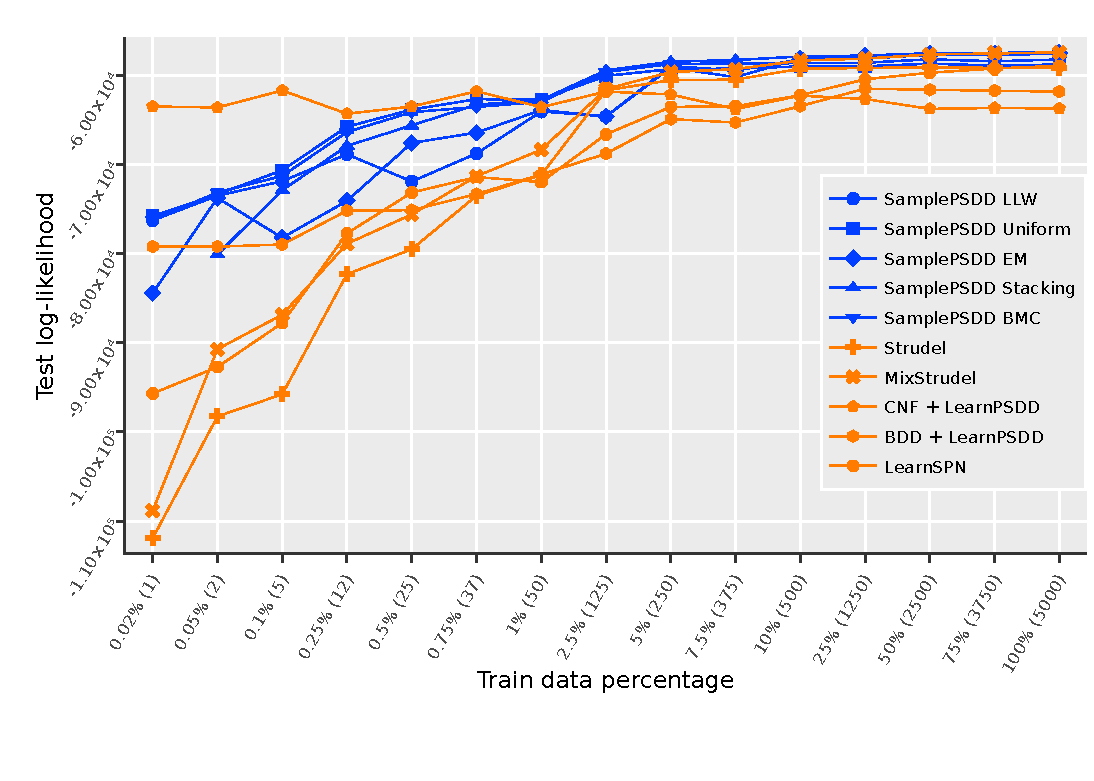
\includegraphics[width=0.765\textwidth]{figures/bic_ll_led_ensembles.pdf}\\
    \vskip -0.97cm
    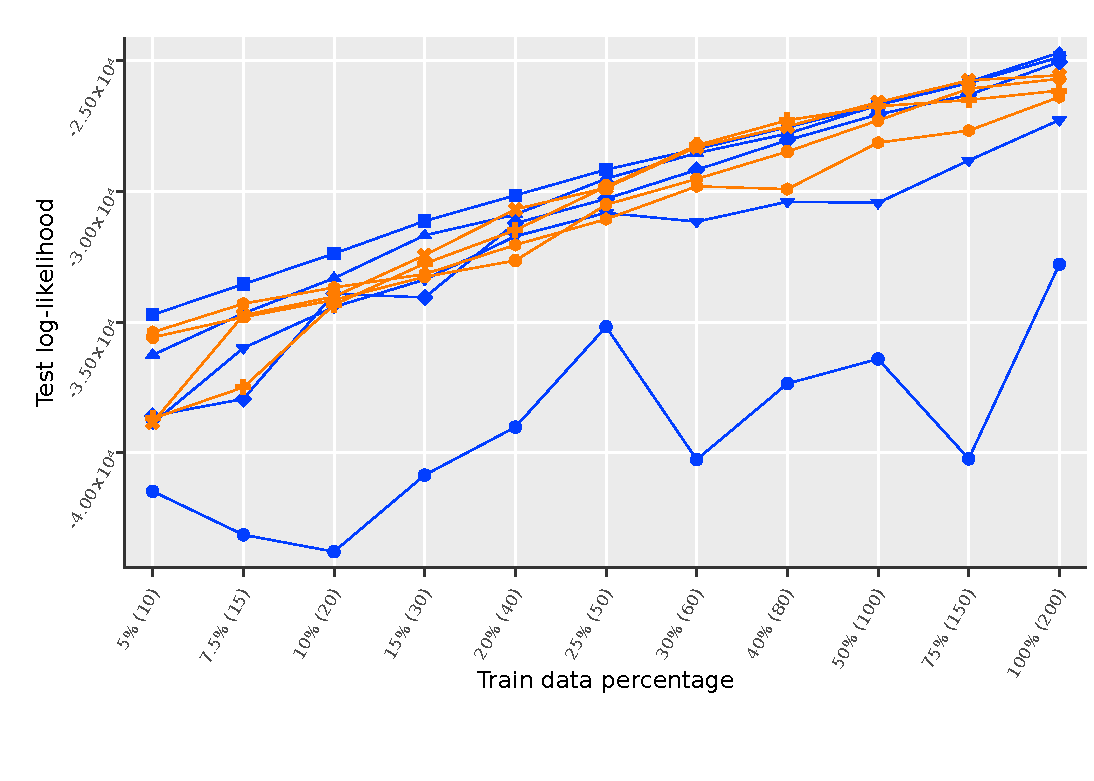
\includegraphics[width=0.765\textwidth]{figures/bic_ll_led_pixels_ensembles.pdf}
  \end{center}
\end{minipage}}

% Slide: SamplePSDD - Experiments 2
\newpage

\newtitle{Experiments}

\vskip 0.25cm
\resizebox{0.495\textwidth}{!}{
\begin{minipage}{0.39\textwidth}
  \noindent
  \colorbox{pyellow}{\textbf{\underline{Evaluation:}}} we sample 30 PSDDs and use 5 ensemble strategies:
  \vskip 0.25cm
  \begin{enumerate}[nosep]
    \item[\llwi]\textcolor{llw}{\textbf{Likelihood weighting (LLW)}},
    \item[\unifi] \textcolor{llw}{\textbf{Uniform weights}},
    \item[\emi] \textcolor{llw}{\textbf{Expectation Maximization (EM)}},
    \item[\stacki] \textcolor{llw}{\textbf{Stacking}},
    \item[\bmci] \textcolor{llw}{\textbf{Bayesian Model Combination (BMC)}};
  \end{enumerate}
  \vskip 0.25cm
  \hskip 0.25cm comparing against \textcolor{unif}{\textbf{\textsc{Strudel}}},
    \textcolor{unif}{\textbf{\textsc{LearnPSDD}}} and \textcolor{unif}{\textbf{\textsc{LearnSPN}}}.
  \vskip 0.25cm
  \colorbox{pyellow}{\textbf{\underline{Datasets:}}} we evaluate with 5 data + knowledge as logic constraints:
  \vskip 0.25cm
  \begin{center}
    \begin{tabular}{cl|rrrr}
      \cline{2-5}
      &\textbf{Dataset} & \textbf{\#vars} & \textbf{\#train} & \textbf{$\phi$'s size}\\
      \cline{2-5}
      &\textsc{LED} & 14 & 5000 & 23 \\
      &\textsc{LED} + \textsc{Images} & 157 & 700 & 39899 \\
      $\Rightarrow$&\textsc{Sushi Ranking} & 100 & 3500 & 17413 \\
      $\Rightarrow$&\textsc{Sushi Top 5} & 10 & 3500 & 37 \\
      &\textsc{Dota 2 Games} & 227 & 92650 & 1308 \\
      \cline{2-5}
    \end{tabular}
  \end{center}
  \begin{align*}
    \text{Our approach }&\text{\colorbox{boxblue!70}{fares \textbf{better} with \textbf{fewer} data}, yet}\\
                        &\text{\colorbox{boxgreen!70}{remains \textbf{competitive} under \textbf{lots of data}}.}
  \end{align*}
  \vskip 0.1cm
  \textcolor{darkgray}{\cite{mattei20b,kamishima03,shen17},}

  \textcolor{darkgray}{\cite{choi15,gens13,dang20}}
\end{minipage}}\resizebox{0.495\textwidth}{!}{\begin{minipage}{0.4\textwidth}
  \begin{center}
    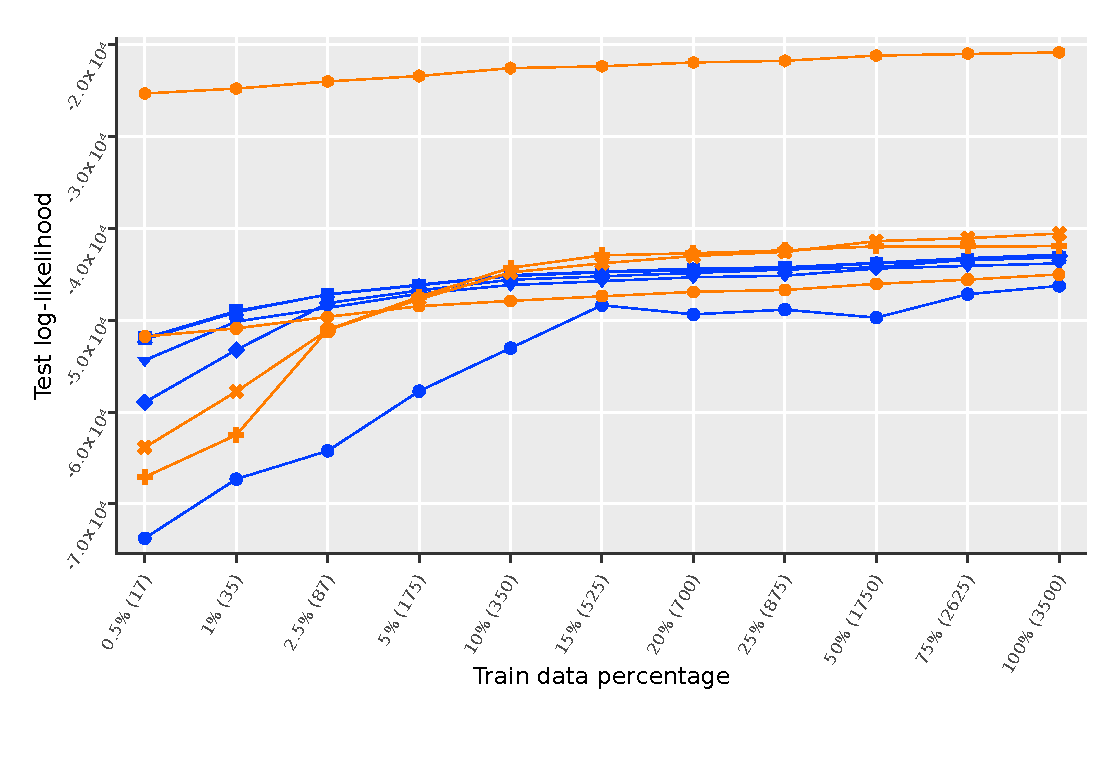
\includegraphics[width=0.765\textwidth]{figures/bic_ll_sushi_ranking_ensembles.pdf}\\
    \vskip -0.97cm
    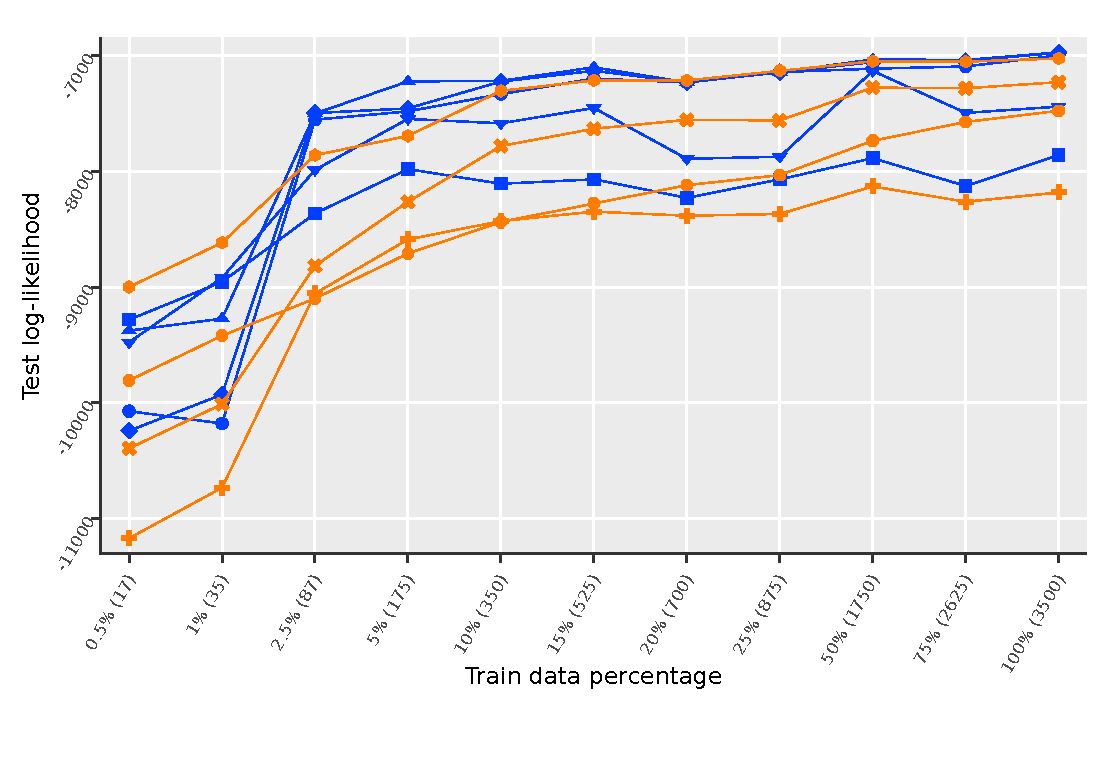
\includegraphics[width=0.765\textwidth]{figures/bic_ll_sushi_choose_ensembles.pdf}
  \end{center}
\end{minipage}}

% Slide: SamplePSDD - Experiments 3
\newpage

\newtitle{Experiments}

\vskip 0.25cm
\resizebox{0.495\textwidth}{!}{
\begin{minipage}{0.39\textwidth}
  \noindent
  \colorbox{pyellow}{\textbf{\underline{Evaluation:}}} we sample 30 PSDDs and use 5 ensemble strategies:
  \vskip 0.25cm
  \begin{enumerate}[nosep]
    \item[\llwi] \textcolor{llw}{\textbf{Likelihood weighting (LLW)}},
    \item[\unifi] \textcolor{llw}{\textbf{Uniform weights}},
    \item[\emi] \textcolor{llw}{\textbf{Expectation Maximization (EM)}},
    \item[\stacki] \textcolor{llw}{\textbf{Stacking}},
    \item[\bmci] \textcolor{llw}{\textbf{Bayesian Model Combination (BMC)}};
  \end{enumerate}
  \vskip 0.25cm
  \hskip 0.25cm comparing against \textcolor{unif}{\textbf{\textsc{Strudel}}},
    \textcolor{unif}{\textbf{\textsc{LearnPSDD}}} and \textcolor{unif}{\textbf{\textsc{LearnSPN}}}.
  \vskip 0.25cm
  \colorbox{pyellow}{\textbf{\underline{Datasets:}}} we evaluate with 5 data + knowledge as logic constraints:
  \vskip 0.25cm
  \begin{center}
    \begin{tabular}{cl|rrrr}
      \cline{2-5}
      &\textbf{Dataset} & \textbf{\#vars} & \textbf{\#train} & \textbf{$\phi$'s size}\\
      \cline{2-5}
      &\textsc{LED} & 14 & 5000 & 23 \\
      &\textsc{LED} + \textsc{Images} & 157 & 700 & 39899 \\
      &\textsc{Sushi Ranking} & 100 & 3500 & 17413 \\
      &\textsc{Sushi Top 5} & 10 & 3500 & 37 \\
      $\Rightarrow$&\textsc{Dota 2 Games} & 227 & 92650 & 1308 \\
      \cline{2-5}
    \end{tabular}
  \end{center}
  \begin{align*}
    \text{Our approach }&\text{\colorbox{boxblue!70}{fares \textbf{better} with \textbf{fewer} data}, yet}\\
                        &\text{\colorbox{boxgreen!70}{remains \textbf{competitive} under \textbf{lots of data}}.}
  \end{align*}
  \vskip 0.1cm
  \textcolor{darkgray}{\cite{mattei20b,kamishima03,shen17},}

  \textcolor{darkgray}{\cite{choi15,gens13,dang20}}
\end{minipage}}\resizebox{0.495\textwidth}{!}{\begin{minipage}{0.4\textwidth}
  \begin{center}
    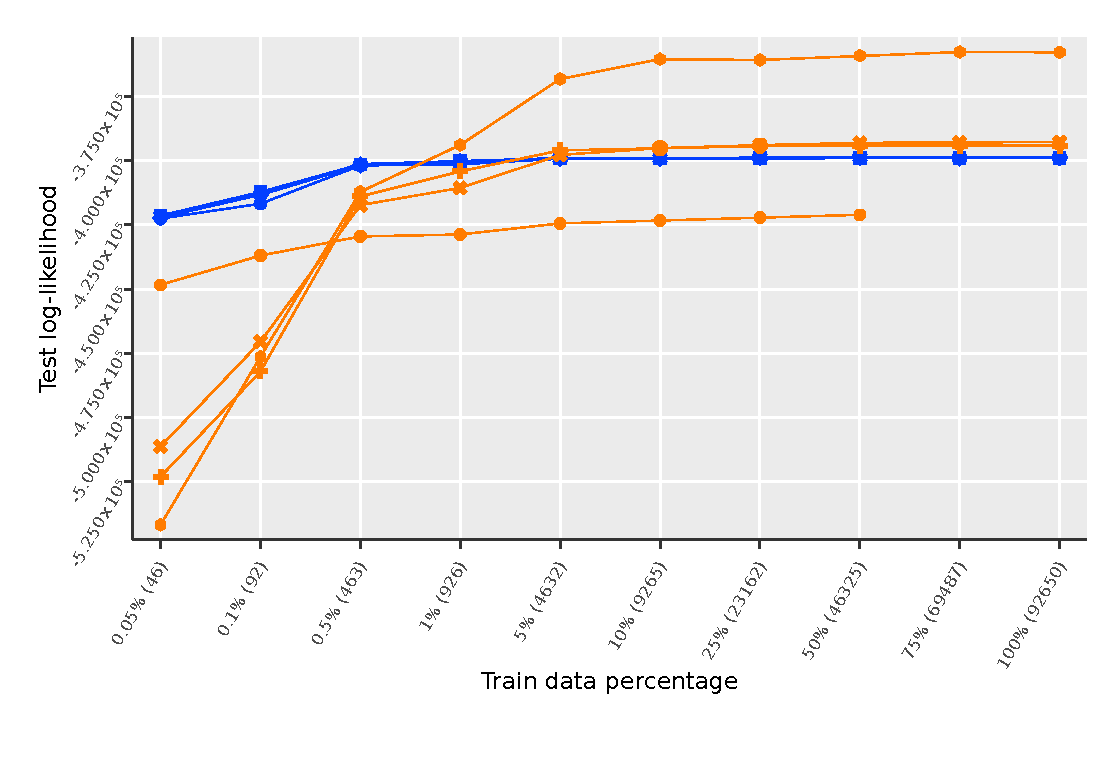
\includegraphics[width=0.765\textwidth]{figures/bic_ll_dota_ensembles.pdf}\\
    \vskip -0.97cm
    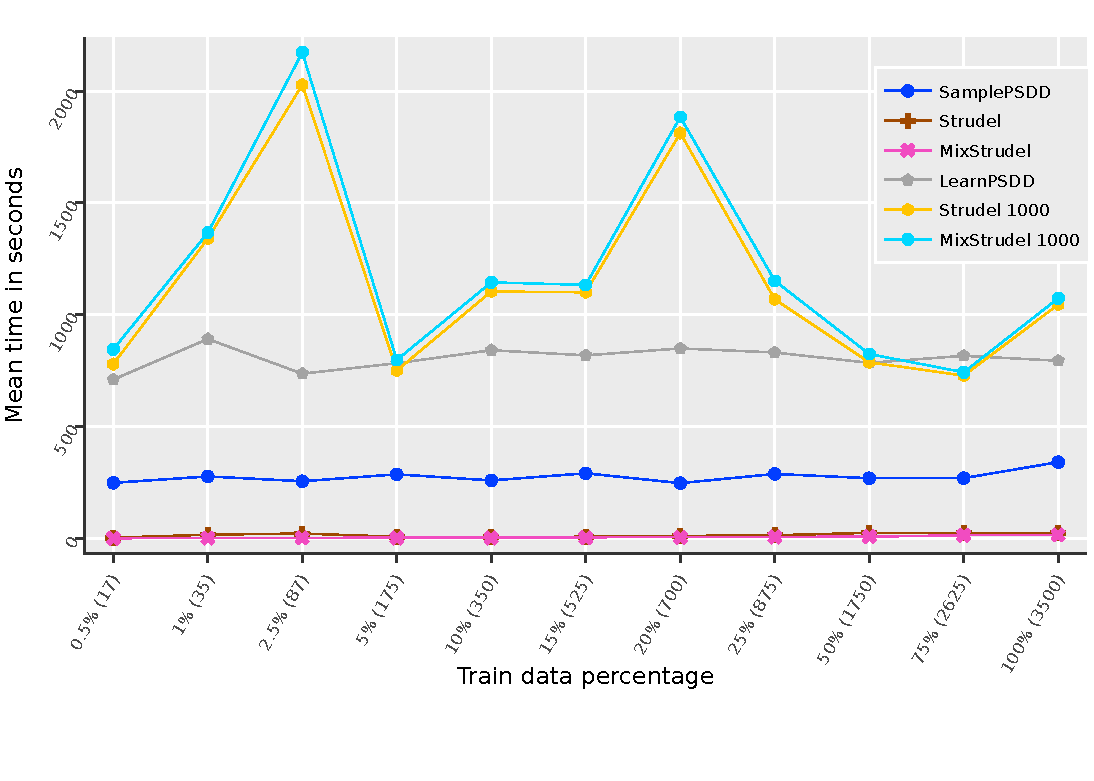
\includegraphics[width=0.765\textwidth]{figures/all_sushi_time.pdf}
  \end{center}
\end{minipage}}

% Slide: SamplePSDD - Experiments 4
\newpage

\newtitle{Experiments}

\begin{center}
\vskip -0.7cm
\resizebox{0.4\textwidth}{!}{
  \begin{minipage}{0.35\textwidth}
    \begin{align*}
      \text{What is the impact of }&\text{\colorbox{boxgreen!70}{higher $k$'s} and \colorbox{pyellow}{right-leaning vtrees}}\\
                         \text{in }&\text{\colorbox{boxblue!70}{log-likelihood} and \colorbox{Red}{\color{white}consistency}}?
    \end{align*}
  \end{minipage}
}
\vskip 0.25cm
\begin{center}
  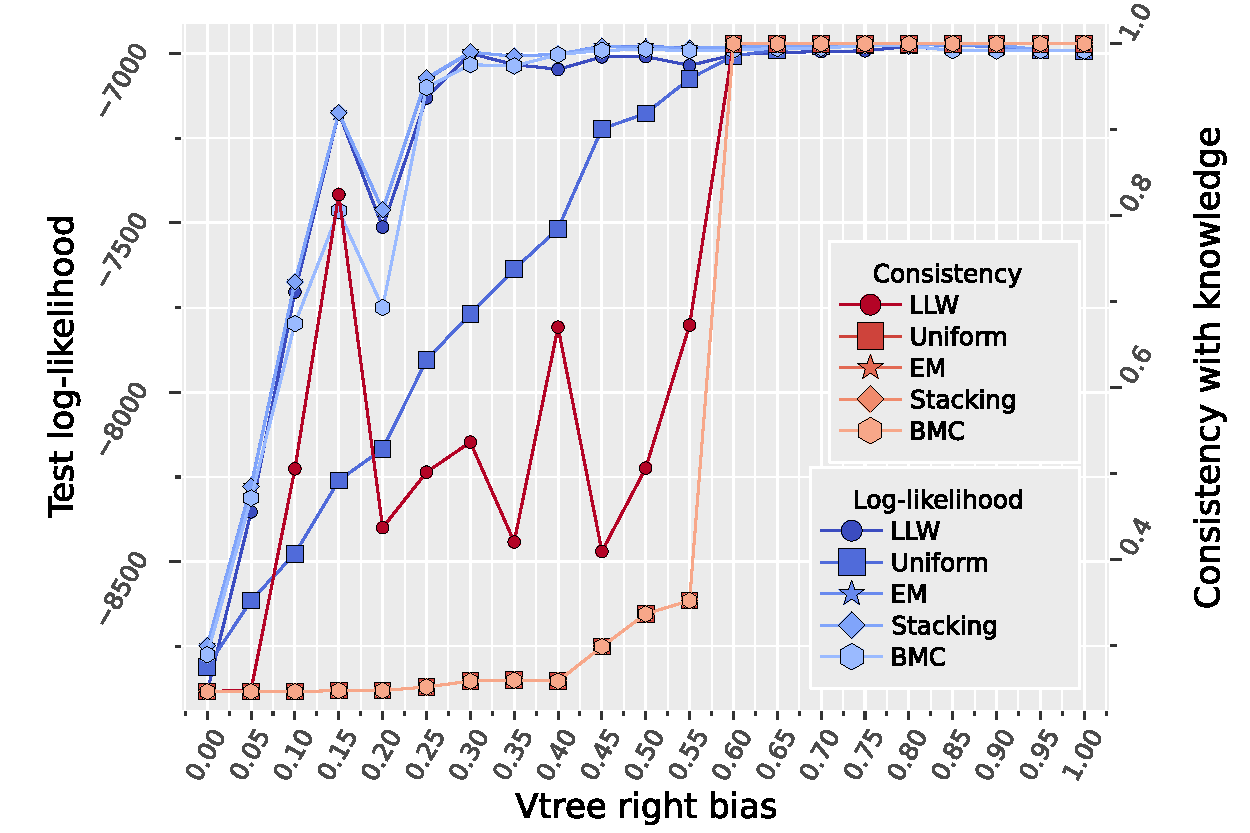
\includegraphics[width=0.3\textwidth]{figures/vtree_ll_imp_sushi.pdf}
  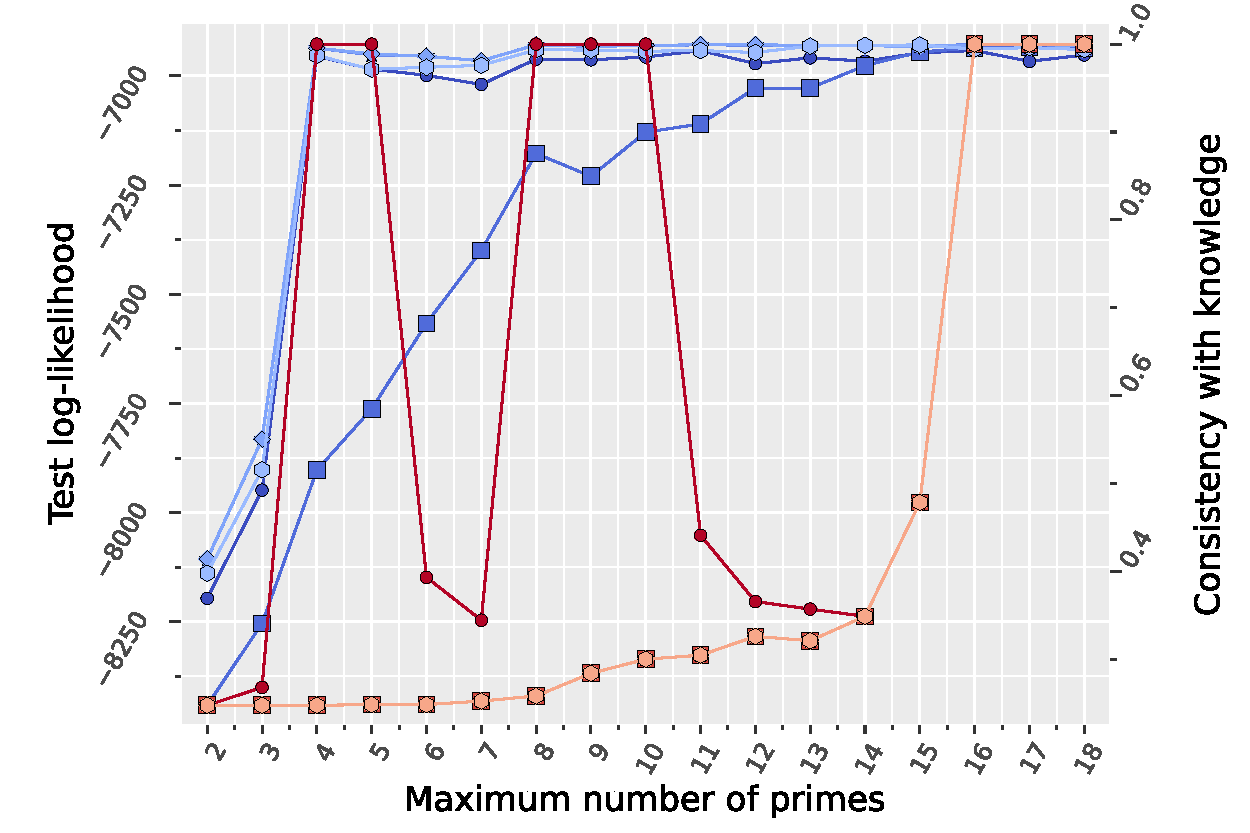
\includegraphics[width=0.3\textwidth]{figures/k_ll_imp_sushi.pdf}
\end{center}
\vskip -0.5cm
\resizebox{0.4\textwidth}{!}{
  \begin{minipage}{0.4\textwidth}
    \begin{align*}
      \text{Samples perform }&\text{\colorbox{boxgreen!70}{\textbf{better} with higher $k$'s} and \colorbox{pyellow}{right-leaning vtrees}...}\\
                   \text{...}&\text{but at a \colorbox{boxorange!70}{\textbf{cost} to complexity}.}
    \end{align*}
  \end{minipage}
}
\begin{center}
  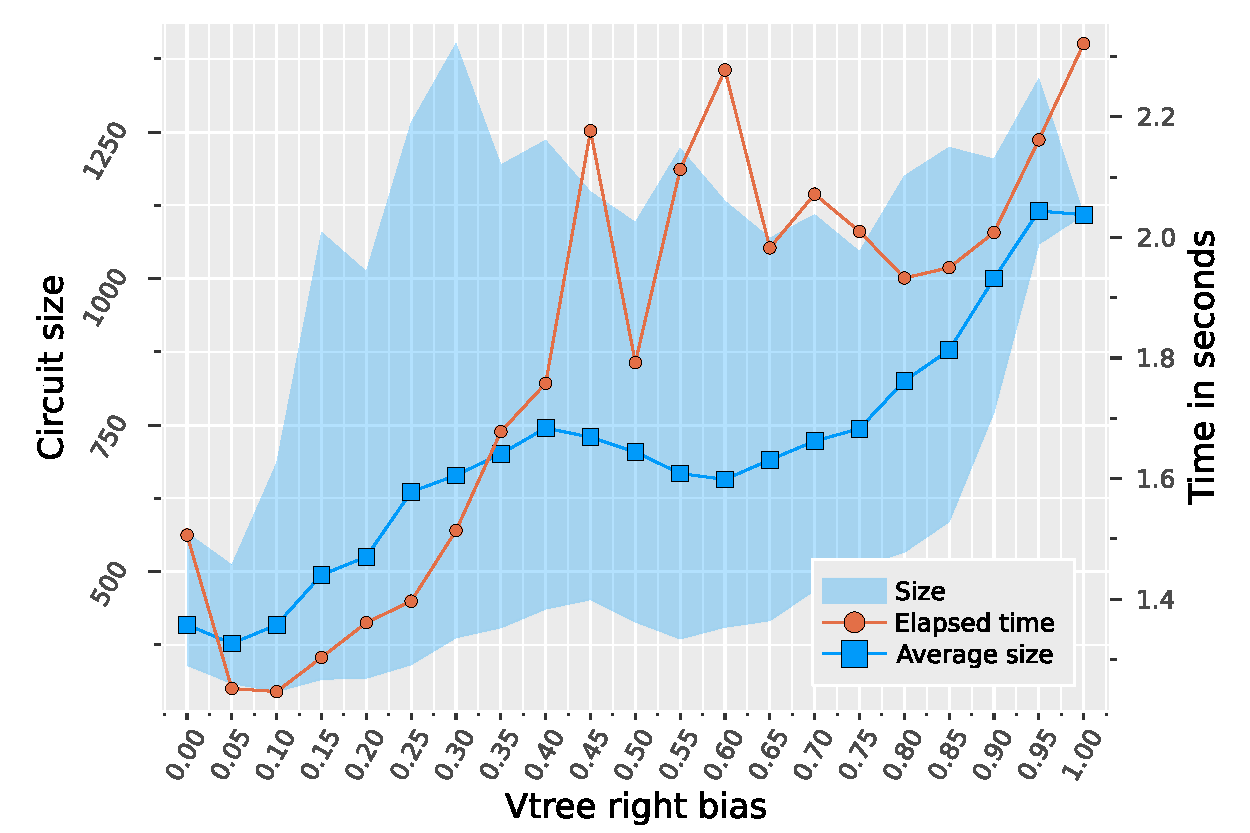
\includegraphics[width=0.3\textwidth]{figures/vtree_complexity.pdf}
  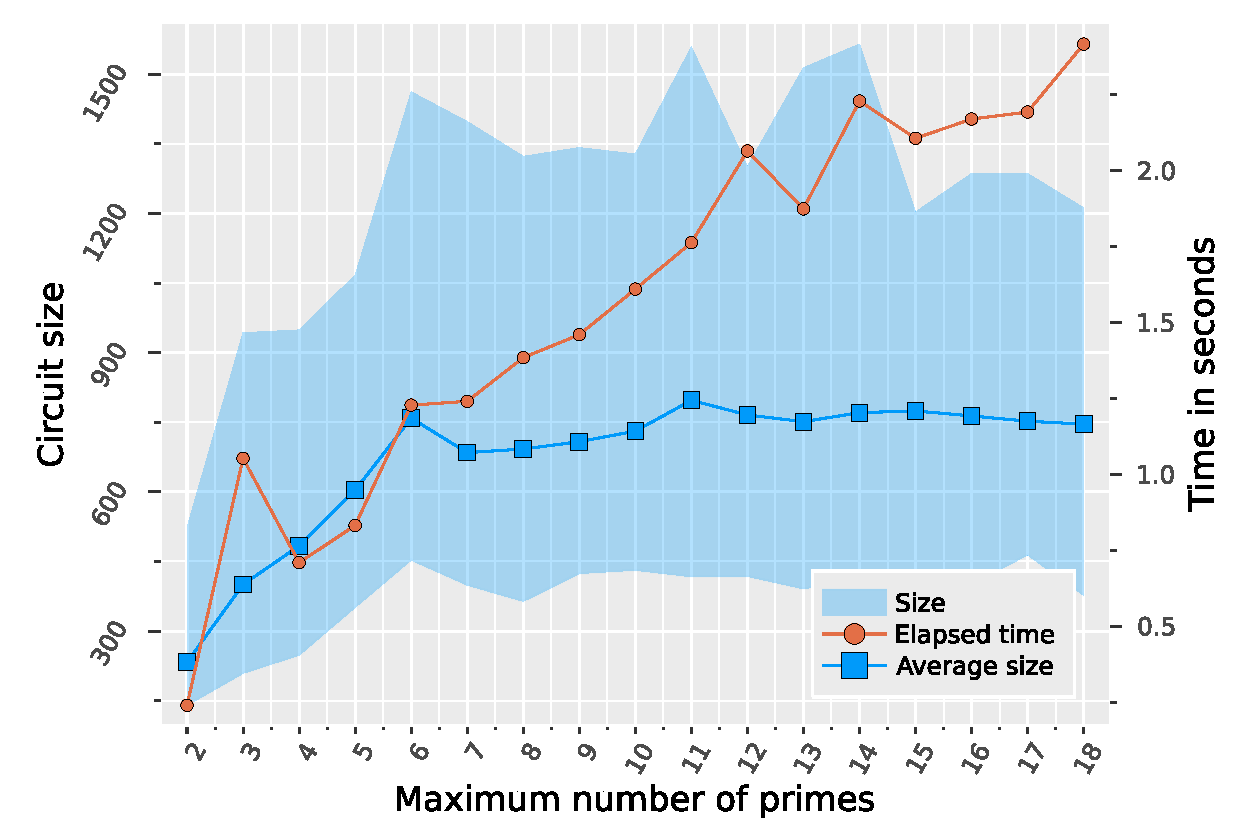
\includegraphics[width=0.3\textwidth]{figures/k_complexity.pdf}
\end{center}
\end{center}

% Slide: SamplePSDD - What do we gain from this?

\newpage

\newtitle{What do we gain from this?}
\vskip 1cm

\begin{minipage}[t]{0.35\textwidth}
  \begin{vhcenterb}
    \parbox{0.9\textwidth}{
    \large
    {\Large{}\textbf{Available queries:}}
    \vskip 0.5cm

    \begin{checks}
      \item[\done] Probability of Evidence;
      \item[\done] Marginal Probability;
      \item[\done] Conditional Probability;
      \item[\done] Most Probable Explanation;
      \item[\done] Shannon Entropy;
      \item[\done] Cross Entropy;
      \item[\done] Kullback-Leibler Divergence;
      \item[\done] Rényi's Alpha Divergence;
      \item[\done] Cauchy-Schwarz Divergence;
      \item[\done] Probability of Logical Events;
      \item[\done] Mutual Information.
    \end{checks}

    \vskip 0.25cm
    {\Large{}\textbf{Support:}}
    \vskip 0.5cm

    \begin{checks}
      \item[\done] Defineable as a logic formula;
      \item[\wontfix] Consistent with a relaxation;
      \item[\done] Ensembles mitigate relaxation.
    \end{checks}
    }
  \end{vhcenterb}
\end{minipage}
\begin{minipage}[t][0.8\textheight]{0.625\textwidth}
  \begin{vhcenterb}
    \resizebox{\textwidth}{!}{
    \begin{tikzpicture}
      \node (tab) at (-7,-0.5) {
        \begin{tabular}{|ccc|c|} \hline
          $A$ & $B$ & $C$ & $p(\set{x})$\\
          \hline
          0 & 0 & 0 & 0.1\\
          0 & 1 & 0 & 0.1\\
          1 & 0 & 0 & 0.2\\
          1 & 0 & 1 & 0.6\\
          \hline
        \end{tabular}
      };

      \node at ($(tab) + (0,-2)$) {\small$\phi(A,B,C)=(A\to\neg B)\wedge(C\to A)$};

      \newVtreeNode{v_root}{$(tab) + (0,-3)$}{1};
      \newVtreeNode[fill=boxorange!80]{v_lr}{$(v_root)+(-0.55, -1.5)$}{$A$};
      \newVtreeNode{v_rr}{$(v_root)+(0.55,-1.5)$}{2};
      \newVtreeNode[fill=boxblue!50]{v_lrr}{$(v_root)+(0,-3.0)$}{$B$};
      \newVtreeNode[fill=boxgoldenrod!70]{v_rrr}{$(v_root)+(1.1, -3.0)$}{$C$};
      \draw (v_root) -- (v_lr);
      \draw (v_root) -- (v_rr);
      \draw (v_rr) -- (v_lrr);
      \draw (v_rr) -- (v_rrr);

      \newNamedOrNode[fill=boxgreen,inputs=nn]{r}{0,0}{1};
      \newAndNode[fill=boxpink!80,inputs=nn]{p1}{$(r) + (-0.75,-1.5)$};
      \newAndNode[fill=boxred,inputs=nn]{p2}{$(r) + (0.75,-1.5)$};
      \newNamedOrNode[fill=boxolive,inputs=nn]{s1}{$(p1.input 2) + (0,-1.0)$}{2};
      \newNamedOrNode[fill=boxmunsel,inputs=nn]{s2}{$(p2.input 2) + (2.2,-1.0)$}{2};
      \newAndNode[inputs=nn]{s1p1}{$(r) + (-1.5,-4.25)$};
      \newAndNode[inputs=nn]{s2p1}{$(r) + (2.1,-4.5)$};
      \newAndNode[inputs=nn]{s2p2}{$(r) + (3.9,-4.5)$};
      \newOrNode[inputs=nn]{s3}{$(r) + (-0.25,-5.5)$};

      \node[fill=boxorange!80,minimum size=17pt,label=center:{$A$}] (p1l) at ($(p1.input 1) + (-0.75,-1.0)$) {};
      \node[fill=boxorange!80,minimum size=17pt,label=center:{$\neg A$}] (p2l) at ($(p2.input 1) + (0.0,-1.0)$) {};
      \node[fill=boxblue!50,minimum size=17pt,label=center:{$\neg B$}] (s1p1l) at ($(s1p1.input 1) + (-0.75,-0.75)$) {};
      \node[fill=boxblue!50,minimum size=17pt,label=center:{$\neg B$}] (s2p1l1) at ($(s2p1.input 1) + (-0.5,-1.0)$) {};
      \node[fill=boxgoldenrod!70,minimum size=17pt,label=center:{$\neg C$}] (s2p1l2) at ($(s2p1.input 2) + (0.5,-1.0)$) {};
      \node[fill=boxblue!50,minimum size=17pt,label=center:{$B$}] (s2p2l1) at ($(s2p2.input 1) + (-0.5,-1.0)$) {};
      \node[fill=boxgoldenrod!70,minimum size=17pt,label=center:{$\neg C$}] (s2p2l2) at ($(s2p2.input 2) + (0.5,-1.0)$) {};
      \node[fill=boxgoldenrod!70,minimum size=17pt,label=center:{$C$}] (s3l1) at ($(s3.input 1) + (-0.5,-1.0)$) {};
      \node[fill=boxgoldenrod!70,minimum size=17pt,label=center:{$\neg C$}] (s3l2) at ($(s3.input 2) + (0.5,-1.0)$) {};

      \draw[edge] (r.input 1) -- ++(0,-0.4) -| node[above left]{\color{pdgreen}$.8$} (p1.east);
      \draw[edge] (r.input 2) -- ++(0,-0.4) -| node[above right]{\color{pdgreen}$.2$} (p2.east);
      \draw[edge] (p1.input 1) -- ++(0,-0.4) -| (p1l.north);
      \draw[edge] (p2.input 1) -- ++(0,-0.4) -| (p2l.north);
      \draw[edge] (s1p1.input 1) -- ++(0,-0.2) -| (s1p1l.north);
      \draw[edge] (s2p1.input 1) -- ++(0,-0.4) -| (s2p1l1.north);
      \draw[edge] (s2p1.input 2) -- ++(0,-0.4) -| (s2p1l2.north);
      \draw[edge] (s2p2.input 1) -- ++(0,-0.4) -| (s2p2l1.north);
      \draw[edge] (s2p2.input 2) -- ++(0,-0.4) -| (s2p2l2.north);
      \draw[edge] (s3.input 1) -- ++(0,-0.4) -| node[above left]{\color{pdgreen}$.75$} (s3l1.north);
      \draw[edge] (s3.input 2) -- ++(0,-0.4) -| node[above right]{\color{pdgreen}$.25$} (s3l2.north);
      \draw[edge] (p1.input 2) -- ++(0,-0.4) -| (s1.east);
      \draw[edge] (p2.input 2) -- ++(0,-0.4) -| (s2.east);
      \draw[edge] (s1.west) -- ++(0,-0.3) node[below right]{\color{pdgreen}$1.0$} -| (s1p1.east);
      \draw[edge] (s2.input 1) -- ++(0,-0.4) -| node[above left]{\color{pdgreen}$.5$} (s2p1.east);
      \draw[edge] (s2.input 2) -- ++(0,-0.4) -| node[above right]{\color{pdgreen}$.5$} (s2p2.east);
      \draw[edge] (s1p1.input 2) -- ++ (0,-0.2) -| (s3.east);

      \node at ($(p1l) + (-0.75,0)$) {\color{pviolet}$p_1$};
      \node at ($(s1) + (0.5,0.5)$) {\color{psandy}$s_1$};
      \node at ($(p2l) + (0.75,0)$) {\color{pviolet}$p_2$};
      \node at ($(s2) + (0.5,0.5)$) {\color{psandy}$s_2$};
    \end{tikzpicture}
    }
  \end{vhcenterb}
\end{minipage}

% Slide: A Data Perspective

\newpage

\begin{vhcenterb}
  \resizebox{!}{3em}{
    \color{boxblue}A Data Perspective
  }
\end{vhcenterb}

% Slide: LearnRP - Motivation 1

\newpage

\newtitle{Motivation}

\begin{vhcenterb}
\begin{minipage}[t][0.8\textheight][t]{0.35\textwidth}
  \vskip 0.5cm

  \large
  {\Large{}\textbf{Density Estimation Trees...}}
  \vskip 0.5cm

  \begin{checks}
    \item[\done] ...are fast;
    \item[\done] ...are interpretable;
    \item[\done] ...are (somewhat) explainable;
    \item[\done] ...have extensive literature coverage;
    \item[\wontfix] ...are not so expressive;
    \item[\wontfix] ...only accept marginalization queries;
    \item[\wontfix] ...are not so accurate;
  \end{checks}
  \vskip 0.15cm
  \textbf{...but are subsumed by circuits!}
  \vskip 1.2cm
  \begin{center}
    \colorbox{boxorange!70}{Learn DETs $\bm{\subseteq}$ Learn PCs?}
  \end{center}
  \vskip 0.7cm

  \begin{center}
    \colorbox{boxteal}{\parbox{0.85\textwidth}{\color{white}\textbf{Can we take advantage of known
    learning\\procedures in DETs and transplant them to\\more general circuits?}}}
  \end{center}
\end{minipage}
\begin{minipage}[t][0.9\textheight][t]{0.3\textwidth}
  \begin{vhcenterb}
    \resizebox{!}{0.8\textheight}{
    \begin{tikzpicture}
      \fill[boxpink!30] (0,0) rectangle (2,2.5);
      \fill[boxgoldenrod!40] (2,0) rectangle (3.5,2.5);
      \draw[very thick,boxblue,dashed] (3.5,0) -- node[left,pos=0.9] {\color{boxblue}$\set{A}$} (3.5,5);
      \draw[very thick,boxgreen,dashed] (0,2.5) -- node[right,pos=1] {\color{boxgreen}$\set{B}$} (3.5,2.5);
      \draw[very thick,boxpurple!80,dashed] (2,0) -- node[above,pos=1] {\color{boxpurple}$\set{C}$} (2,2.5);
      \node at (1,1.25) {$\Leaf_1$};
      \node at (2.75,1.25) {$\Leaf_2$};
      \node[circle,inner sep=0pt,minimum size=3pt,fill=black,label=above right:{$\set{x}$}] at (1.5,1.9) {};
      \draw[very thick] (0,0) rectangle (5, 5);

      \node[inner sep=1pt,minimum size=12pt,circle,fill=boxblue!80] (a) at (3,-1.0) {$\set{A}$}; \node[inner sep=1pt,minimum size=12pt,circle,fill=boxgreen!80] (b) at ($(a) + (-1,-1.5)$) {$\set{B}$};
      \node[inner sep=1pt,minimum size=12pt,circle,fill=boxpurple!60] (c) at ($(b) + (1,-1.5)$) {$\set{C}$};
      \node[draw,fill=boxpink!30] (l1) at ($(c) + (-1,-1.5)$) {$L_1$};
      \node[draw,fill=boxgoldenrod!40] (l2) at ($(c) + (1,-1.5)$) {$L_2$};
      \draw (a) -- node[below,pos=1] {$\vdots$} node[above right,pos=0.5] {$\set{x}\in\set{A}^+$} ($(a) + (1,-1.5)$);
      \draw (a) -- node[above left,pos=0.5] {$\set{x}\in\set{A}^-$} (b);
      \draw[edge,boxdgray] (a) edge[bend left=15] (b);
      \draw (b) -- node[below,pos=1] {$\vdots$} node[above left,pos=0.5] {$\set{x}\in\set{B}^-$} ($(b) + (-1,-1.5)$);
      \draw (b) -- node[above right,pos=0.5] {$\set{x}\in\set{B}^+$} (c);
      \draw[edge,boxdgray] (b) edge[bend right=15] (c);
      \draw (c) -- node[above left,pos=0.5] {$\set{x}\in\set{C}^-$} (l1);
      \draw (c) -- node[above right,pos=0.5] {$\set{x}\in\set{C}^+$} (l2);
      \draw[edge,boxdgray] (c) edge[bend left=15] (l1);
    \end{tikzpicture}
    }
  \end{vhcenterb}
\end{minipage}
\begin{minipage}[t][0.9\textheight][t]{0.3\textwidth}
  \begin{vhcenterb}
    \resizebox{!}{0.8\textheight}{
    \begin{tikzpicture}
      \newSumNode[fill=boxblue!80,label=above left:{\color{boxblue}$\set{A}$}]{a}{9,2};
      \newProdNode[fill=boxblue!80]{al}{$(a) + (-0.5,-1)$};
      \newProdNode[fill=boxblue!80]{ar}{$(a) + (0.5,-1)$};
      \newLeafNode[fill=boxblue!80,label=below:{$\left\liv\set{x}\in\set{A}^-\right\riv$}]{ai}{$(al) + (-1.0,-1)$};
      \newLeafNode[fill=boxblue!80,label=below:{$\left\liv\set{x}\in\set{A}^+\right\riv$}]{nai}{$(ar) + (1.0,-1)$};
      \draw[edge] (a) -- (al); \draw[edge] (al) -- (ai);
      \draw[edge] (a) -- (ar); \draw[edge] (ar) -- (nai);
      \draw[edge] (ar) -- node[inner sep=0pt,below,pos=1] {$\vdots$} ($(ar) + (0,-0.8)$);

      \newSumNode[fill=boxgreen!80,label=above right:{\color{boxgreen}$\set{B}$}]{b}{$(al) + (0,-1)$};
      \newProdNode[fill=boxgreen!80]{bl}{$(b) + (0,-1)$};
      \newProdNode[fill=boxgreen!80]{br}{$(b) + (1,-1)$};
      \newLeafNode[fill=boxgreen!80,label=below:{$\left\liv\set{x}\in\set{B}^-\right\riv$}]{bi}{$(bl) + (-1.0,-1)$};
      \newLeafNode[fill=boxgreen!80,label=below:{$\left\liv\set{x}\in\set{B}^+\right\riv$}]{nbi}{$(br) + (1.0,-1)$};
      \draw[edge] (al) -- (b);
      \draw[edge] (b) -- (bl); \draw[edge] (bl) -- (bi);
      \draw[edge] (b) -- (br); \draw[edge] (br) -- (nbi);
      \draw[edge] (bl) -- node[inner sep=0pt,below,pos=1] {$\vdots$} ($(bl) + (0,-0.8)$);

      \newSumNode[fill=boxpurple!60,label=above left:{\color{boxpurple}$\set{C}$}]{c}{$(br) + (0,-1)$};
      \newProdNode[fill=boxpurple!60]{cl}{$(c) + (-1,-1)$};
      \newProdNode[fill=boxpurple!60]{cr}{$(c) + (0,-1)$};
      \newLeafNode[fill=boxpurple!60,label=below:{$\left\liv\set{x}\in\set{C}^-\right\riv$}]{ci}{$(cl) + (-1.0,-1)$};
      \newLeafNode[fill=boxpurple!60,label=below:{$\left\liv\set{x}\in\set{C}^+\right\riv$}]{nci}{$(cr) + (1.0,-1)$};
      \draw[edge] (br) -- (c);
      \draw[edge] (c) -- (cr); \draw[edge] (cl) -- (ci);
      \draw[edge] (c) -- (cl); \draw[edge] (cr) -- (nci);
      \newGaussNode[label=below:{$\Leaf_1$},fill=boxpink!30]{l1}{$(cl) + (0,-1)$};
      \newGaussNode[label=below:{$\Leaf_2$},fill=boxgoldenrod!40]{l2}{$(cr) + (0,-1)$};
      \draw[edge] (cl) -- (l1);
      \draw[edge] (cr) -- (l2);
    \end{tikzpicture}
    }
  \end{vhcenterb}
\end{minipage}
\end{vhcenterb}

\vskip -2cm
{\color{boxdgray}\cite{correia20,ram11}}

% Slide: LeanrRP - Random Projections

\newpage

\newtitle{Random Projections}

\begin{vhcenterb}
  \def\points{(2.3,4.38),(1.8,4.0),(2.8,4.0),(1.6,3.3),(2.5,3),(3.1,2.8),(3.8,3.1),(4.3,3.3),(4,2.6),(4.5,2.4),(3.3,2.3),(2.1,2.0),(3.1,1.8),(2.4,1.6),(2.9,1.5),(2.5,1.3),(3.1,1.1),(3.1,0.6),(2.7,0.8),(1.5,0.8),(1.7,1.3),(1.2,1.5),(3.6,0.5),(4,0.3),(4.1,0.6),(3.8,0.8),(4.4,0.8),(4,1.1),(4.3,1.1),(4.6,1),(3.6,1.2),(3.9,1.4),(4.2,1.4),(4.6,1.4),(4.4,1.7),(3.8,1.7)}

  \begin{minipage}[t]{0.25\textwidth}
    \centering
    \resizebox{\textwidth}{!}{
    \begin{tikzpicture}
      \foreach \p in \points {
        \node[circle,inner sep=0pt,minimum size=2pt,fill=boxgray] at \p {};
      }
      \draw[very thick,boxblue,dashed] (3.5,0) -- node[left,pos=0.9] {\color{boxblue}$\set{A}$} (3.5,5);
      \draw[very thick,boxgreen,dashed] (0,2.5) -- node[right,pos=1] {\color{boxgreen}$\set{B}$} (3.5,2.5);
      \draw[very thick,boxpurple!80,dashed] (2,0) -- node[above,pos=1] {\color{boxpurple}$\set{C}$} (2,2.5);
      \draw[very thick,boxmunsel,dashed] (0,3.75) -- node[right,pos=1] {\color{boxmunsel}$\set{D}$} (3.5,3.75);
      \draw[very thick,boxolive!80!black,dashed] (3.5,2) -- node[below,pos=0.5] {\color{boxolive!80!black}$\set{E}$} (5,2);
      \draw[very thick] (0,0) rectangle (5, 5);
      \node at (2.5, -0.5) {\emph{Axis-aligned projections}};
    \end{tikzpicture}
    }
  \end{minipage}
  \hspace{3cm}
  \begin{minipage}[t]{0.25\textwidth}
    \centering
    \resizebox{\textwidth}{!}{
    \begin{tikzpicture}
      \foreach \p in \points {
        \node[circle,inner sep=0pt,minimum size=2pt,fill=boxgray] at \p {};
      }
      \draw[very thick,boxblue,dashed] (2.2,0) coordinate (a1) -- node[left,pos=0.9] {\color{boxblue}$\set{A}$} (5,3.1) coordinate (a2);
      \draw[very thick,boxgreen,dashed] ($(a1)!0.5!(a2)$) coordinate (b1) -- node[above right,pos=0.9] {\color{boxgreen}$\set{B}$} (0,4.2) coordinate (b2);
      \draw[very thick,boxpurple!80,dashed] ($(b1)!0.35!(b2)$) coordinate (c1) -- node[above left,pos=0.7] {\color{boxpurple}$\set{C}$} (5,5) coordinate (c2);
      \draw[very thick,boxmunsel,dashed] ($(b1)!0.22!(b2)$) coordinate (d1) -- node[above left,pos=0.9] {\color{boxmunsel}$\set{D}$} (1.8,0) coordinate (d2);
      \draw[very thick,boxolive!80!black,dashed] ($(a1)!0.45!(a2)$) -- node[right,pos=0.6] {\color{boxolive!80!black}$\set{E}$} (5,0);
      \draw[very thick] (0,0) rectangle (5, 5);
      \node at (2.5, -0.5) {\emph{Random projections}};
    \end{tikzpicture}
    }
  \end{minipage}

  \vskip 1.5cm
  \Large
  \begin{minipage}{0.75\textwidth}
    \begin{quote}
      If the data has \emph{intrinsic dimension} $d$, then with constant probability the part of
      the data at level $d$ or higher of the tree has average diameter less than half of the data.
    \end{quote}
  \end{minipage}
\end{vhcenterb}

{\color{boxdgray}\cite{dasgupta08a,dasgupta08b}}

% Slide: LeanrRP - Random Projections

\newpage

\newtitle{Random Projections}

\begin{vhcenterb}
  \def\points{(2.3,4.38),(1.8,4.0),(2.8,4.0),(1.6,3.3),(2.5,3),(3.1,2.8),(3.8,3.1),(4.3,3.3),(4,2.6),(4.5,2.4),(3.3,2.3),(2.1,2.0),(3.1,1.8),(2.4,1.6),(2.9,1.5),(2.5,1.3),(3.1,1.1),(3.1,0.6),(2.7,0.8),(1.5,0.8),(1.7,1.3),(1.2,1.5),(3.6,0.5),(4,0.3),(4.1,0.6),(3.8,0.8),(4.4,0.8),(4,1.1),(4.3,1.1),(4.6,1),(3.6,1.2),(3.9,1.4),(4.2,1.4),(4.6,1.4),(4.4,1.7),(3.8,1.7)}

  \begin{minipage}[t]{0.25\textwidth}
    \centering
    \resizebox{\textwidth}{!}{
    \begin{tikzpicture}
      \begin{axis}[
        title={\textproc{SplitMax}},
        tick style={draw=none},
        ytick=\empty,
        xtick=\empty,
        enlargelimits=0,
        ymin=-1.8,
        ymax=1.8,
        xmin=-1.8,
        xmax=1.8,
      ]
        \addplot[only marks, olive, opacity=0.5] table {data/max_1_full_parts.data};
        \addplot[only marks, teal, opacity=0.5] table {data/max_2_full_parts.data};
        \addplot[only marks, magenta, opacity=0.5] table {data/max_3_full_parts.data};
        \addplot[only marks, violet, opacity=0.5] table {data/max_4_full_parts.data};
        \addplot[black, thick] coordinates {
          (-0.7435410726460153, 0.2259926265097693)
          (2, -1.906932050205991)
        };
        \addplot[black, thick] coordinates {
          (-0.5739178598189635, 0.33907476839447037)
          (-2, 2.4781979786660253)
        };
        \addplot[black,thick] coordinates {
          (-2, -0.6116466583928871)
          (2, 2.0550200082737793)
        };
      \end{axis}
    \end{tikzpicture}
    }
  \end{minipage}
  \hspace{3cm}
  \begin{minipage}[t]{0.25\textwidth}
    \centering
    \resizebox{\textwidth}{!}{
    \begin{tikzpicture}
      \begin{axis}[
        title={\textsc{SplitSID}},
        tick style={draw=none},
        ytick=\empty,
        xtick=\empty,
        enlargelimits=0,
        ymin=-1.8,
        ymax=1.8,
        xmin=-1.8,
        xmax=1.8
      ]
        \addplot[only marks, olive, opacity=0.5] table {data/sid_1_full_parts.data};
        \addplot[only marks, teal, opacity=0.5] table {data/sid_2_full_parts.data};
        \addplot[only marks, magenta, opacity=0.5] table {data/sid_3_full_parts.data};
        \addplot[only marks, violet, opacity=0.5] table {data/sid_4_full_parts.data};
        \addplot[black, thick] coordinates {
        (-2, -1.3212366499672479)
        (2, 1.3454300166994186)
        };
        \addplot[black, thick] coordinates {
        (-2, 2.346171790525994)
        (-0.3073499505415808, -0.19280328366163507)
        };
        \addplot[black,thick] coordinates {
        (-0.023469760285374355, -0.003549823490830769)
        (2, -1.576665905962419)
        };
      \end{axis}
    \end{tikzpicture}
    }
  \end{minipage}

  \vskip 3cm
  \Large
  \begin{minipage}{0.75\textwidth}
    \begin{quote}
      If the data has \emph{intrinsic dimension} $d$, then with constant probability the part of
      the data at level $d$ or higher of the tree has average diameter less than half of the data.
    \end{quote}
  \end{minipage}
\end{vhcenterb}

{\color{boxdgray}\cite{dasgupta08a,dasgupta08b}}

% Slide: LearnRP 1

\newpage

\newtitle{LearnRP}
\vskip 1cm

\begin{center}
  \begin{minipage}[t][0.7\textheight][t]{0.45\textwidth}
    \vfill
    \begin{vhcenterb}
      \resizebox{0.7\textwidth}{!}{
      \begin{tikzpicture}
        \begin{axis}[
          xmin=0,xmax=5,ymin=0,ymax=5,zmin=0,zmax=5,
          xlabel=$X$,ylabel=$Y$,zlabel=$Z$,zlabel style={rotate=-90},
          xtick={0,1,...,5},ytick={1,...,5},ztick={1,...,5},
          grid=major,
        ]
          \addplot3+[only marks,mark options={boxdgray,fill=boxdgray}] table{data/cloud.dat};
        \end{axis}
      \end{tikzpicture}
      }
    \end{vhcenterb}
  \end{minipage}
  \begin{minipage}[t][0.7\textheight][t]{0.45\textwidth}
    \begin{vhcenterb}
      \resizebox{0.3\textwidth}{!}{
      \begin{tikzpicture}
        \newVtreeNode{v}{0,0}{1};
        \newVtreeNode{z}{$(v) + (-0.5,-1)$}{$Z$};
        \newVtreeNode{r}{$(v) + (0.5,-1)$}{2};
        \newVtreeNode{y}{$(r) + (-0.5,-1)$}{$Y$};
        \newVtreeNode{x}{$(r) + (0.5,-1)$}{$X$};
        \draw (v) -- (z); \draw (v) -- (r);
        \draw (r) -- (y);
        \draw (r) -- (x);
      \end{tikzpicture}
      }
      \vskip 3cm
      \resizebox{0.1\textwidth}{!}{
      \begin{tikzpicture}
        \newSumNode[fill=boxgreen]{r}{0,0};
      \end{tikzpicture}
      }
    \end{vhcenterb}
  \end{minipage}
\end{center}

% Slide: LearnRP 2

\newpage

\newtitle{LearnRP}
\vskip 1cm

\begin{center}
  \def\points{(2.3,4.38),(1.8,4.0),(2.8,4.0),(1.6,3.3),(2.5,3),(3.1,2.8),(3.8,3.1),(4.3,3.3),(4,2.6),(4.5,2.4),(3.3,2.3),(2.1,2.0),(3.1,1.8),(2.4,1.6),(2.9,1.5),(2.5,1.3),(3.1,1.1),(3.1,0.6),(2.7,0.8),(1.5,0.8),(1.7,1.3),(1.2,1.5),(3.6,0.5),(4,0.3),(4.1,0.6),(3.8,0.8),(4.4,0.8),(4,1.1),(4.3,1.1),(4.6,1),(3.6,1.2),(3.9,1.4),(4.2,1.4),(4.6,1.4),(4.4,1.7),(3.8,1.7)}
  \begin{minipage}[t][0.7\textheight][t]{0.45\textwidth}
    \vfill
    \begin{vhcenterb}
      \def\prx{-0.31}
      \def\pry{-0.4}
      \def\prz{0.85}
      \def\prtheta{-1}
      \resizebox{0.7\textwidth}{!}{
      \begin{tikzpicture}
        \begin{axis}[
          xmin=0,xmax=5,ymin=0,ymax=5,zmin=0,zmax=5,
          xlabel=$X$,ylabel=$Y$,zlabel=$Z$,zlabel style={rotate=-90},
          xtick={0,1,...,5},ytick={1,...,5},ztick={1,...,5},
          grid=major,
        ]

          \addplot3+[only marks,mark options={boxblue,fill=boxblue}] table {data/cloud_pos.dat};
          \addplot3+[only marks,mark options={boxred,fill=boxred}] table {data/cloud_neg.dat};
          \addplot3[colormap={bgreen}{color=(boxgreen),color=(boxgreen)},surf,color=boxgreen,
            point meta=1,z buffer=sort,shader=interp,opacity=0.6]
            {-(\prx*x+\pry*y+\prtheta)/\prz};
          \node at (5,3.5,3) {\color{boxgreen}$\set{A}$};
        \end{axis}
      \end{tikzpicture}
      }
      \vskip 0.5cm
      \LARGE
      \begin{equation*}
        \textcolor{boxgreen}{\set{A}}(x,y,z)=\begin{bmatrix} x & y &
          z\\\end{bmatrix}\cdot\scalebox{0.75}{$\begin{bmatrix*}[r]
          -0.31\\ -0.40\\ 0.85 \end{bmatrix*}$}+1
      \end{equation*}
    \end{vhcenterb}
  \end{minipage}
  \begin{minipage}[t][0.7\textheight][t]{0.45\textwidth}
    \begin{vhcenterb}
      \resizebox{0.3\textwidth}{!}{
      \begin{tikzpicture}
        \newVtreeNode[double color fill={boxblue}{boxred},shading angle=45]{v}{0,0}{1};
        \newVtreeNode{z}{$(v) + (-0.5,-1)$}{$Z$};
        \newVtreeNode{r}{$(v) + (0.5,-1)$}{2};
        \newVtreeNode{y}{$(r) + (-0.5,-1)$}{$Y$};
        \newVtreeNode{x}{$(r) + (0.5,-1)$}{$X$};
        \draw (v) -- (z); \draw (v) -- (r);
        \draw (r) -- (y);
        \draw (r) -- (x);
      \end{tikzpicture}
      }
      \vskip 2cm
      \resizebox{0.5\textwidth}{!}{
      \begin{tikzpicture}
        \newSumNode[fill=boxgreen,label=above left:{\color{boxgreen}$\set{A}$}]{r}{0,0};
        \newProdNode[label=below:{$\textcolor{boxgreen}{\set{A}}(\set{x})>0$},fill=boxblue]{p1}{$(r) + (-1,-1)$};
        \newProdNode[label=below:{$\textcolor{boxgreen}{\set{A}}(\set{x})\leq 0$},fill=boxred]{p2}{$(r) + (1,-1)$};
        \draw[edge] (r) -- node[pos=0.5,above left] {$w_{\textcolor{boxgreen}{\set{A}}}=\frac{16}{36}$} (p1);
        \draw[edge] (r) -- node[pos=0.5,above right] {$w_{\textcolor{boxgreen}{\overline{\set{A}}}}=\frac{20}{36}$} (p2);
      \end{tikzpicture}
      }
      \vskip 0.25cm
      \Large
      \begin{equation*}
        w_{\textcolor{boxgreen}{\set{A}}}\text{:\, probability of }\textcolor{boxgreen}{\set{A}}(\set{x})>0
      \end{equation*}
    \end{vhcenterb}
  \end{minipage}
\end{center}

% Slide: LearnRP 3

\newpage

\newtitle{LearnRP}

\begin{center}
  \def\points{(1.6,3.3),(2.5,3),(3.8,3.1),(4.3,3.3),(4,2.6),(3.3,2.3),(3.1,1.8),(2.7,0.8),(4,0.3),(4.1,0.6),(4.4,0.8),(4,1.1),(4.3,1.1),(4.6,1),(4.4,1.7),(3.8,1.7)}

  \begin{minipage}[t][0.7\textheight][t]{0.45\textwidth}
    \vfill
    \begin{vhcenterb}
      \def\prx{-0.31}
      \def\pry{-0.4}
      \def\prz{0.85}
      \def\prtheta{-1}
      \resizebox{0.6\textwidth}{!}{
      \begin{tikzpicture}
        \begin{axis}[
          xmin=0,xmax=5,ymin=0,ymax=5,zmin=0,zmax=5,
          xlabel=$X$,ylabel=$Y$,zlabel=$Z$,zlabel style={rotate=-90},
          xtick={0,1,...,5},ytick={1,...,5},ztick={1,...,5},
          grid=major,
        ]
          \addplot3+[only marks,ycomb,color=boxblue,mark options={boxblue,fill=boxblue}] table {data/cloud_pos.dat};
          \addplot3+[only marks,mark options={boxred,fill=boxred},opacity=0.5] table {data/cloud_neg.dat};
          \addplot3+[only marks,mark options={boxdgray,fill=boxdgray},mark size=1] table[z expr=0] {data/cloud_pos.dat};
          \addplot3+[only marks,mark options={boxorange,fill=boxorange},mark size=2,mark=triangle*] table[x expr=0] {data/cloud_pos.dat};
          \addplot3[colormap={bgreen}{color=(boxgreen),color=(boxgreen)},surf,color=boxgreen,
            point meta=1,z buffer=sort,shader=interp,opacity=0.6]
            {-(\prx*x+\pry*y+\prtheta)/\prz};
          \node at (5,3.5,3) {\color{boxgreen}$\set{A}$};
          \draw[very thick,boxpink,dashed] (2.2,0,0) coordinate (b1) -- node[above left,pos=0.9] {\color{boxpink}$\set{B}$} (5,3.1,0) coordinate (b2);
          \begin{scope}[on background layer]
            \fill[boxblue!50] (0,0,0) -- (b1) -- (b2) -- (5,5,0) -- (0,5,0) -- cycle;
            \fill[boxred!50] (b1) -- (5,0,0) -- (b2) -- cycle;
          \end{scope}
        \end{axis}
      \end{tikzpicture}
      }
      \vskip 0.1cm
      \resizebox{0.95\textwidth}{!}{
        \begin{tikzpicture}
          \coordinate (b1) at (2.2,0);
          \coordinate (b2) at (5,3.1);
          \fill[boxblue!50] (0,0) -- (b1) -- (b2) -- (5,5) -- (0,5) -- cycle;
          \fill[boxred!50] (b1) -- (5,0) -- (b2) -- cycle;
          \foreach \p in \points {
            \node[circle,inner sep=0pt,minimum size=2pt,fill=boxdgray] at \p {};
          }
          \draw[very thick,boxpink,dashed] (b1) -- node[left,pos=0.9] {\color{boxpink}$\set{B}$} (b2);
          \draw[very thick] (0,0) rectangle (5, 5);

          \begin{axis}[
            xshift=6cm,
            samples=30,domain=0:7, axis lines*=left,
            every axis x label/.style={at=(current axis.right of origin),anchor=west},
            every axis y label/.style={at={(axis description cs:0,1)},anchor=south},
            enlargelimits=false, clip=false, axis on top,
            xmin=0,xmax=7,ymin=0,ymax=1,
            xlabel=$Z$,ylabel=$p(Z)$,,xtick={1,...,7},
            grid=major,height=6.45cm,
          ]
            \addplot[only marks,mark options={boxorange,fill=boxorange},mark=triangle*,mark size=4] table[x={z},y expr=0] {data/cloud_pos.dat};
            \path[name path=axis] (axis cs:0,0) -- (axis cs:5,0);
            \addplot[very thick,boxorange,name path=g1] {gauss(3.76,0.95)};
            \addplot[boxorange!60] fill between [of=g1 and axis];
            \node at (3.76,0.5) {$\mathcal{N}(\mu=3.76,\sigma=0.95)$};
          \end{axis}
          \node at (12,0) {};
        \end{tikzpicture}
      }
      \LARGE
      \begin{equation*}
        \textcolor{boxpink}{\set{B}}(x,y)=\begin{bmatrix} x & y\end{bmatrix}\cdot
        \scalebox{0.75}{$\begin{bmatrix*}[r] 1.10\\ -1.00 \end{bmatrix*}$}-2.43
      \end{equation*}
    \end{vhcenterb}
  \end{minipage}
  \begin{minipage}[t][0.7\textheight][t]{0.45\textwidth}
    \begin{vhcenterb}
      \vskip 1cm
      \resizebox{0.3\textwidth}{!}{
      \begin{tikzpicture}
        \newVtreeNode[fill=boxgreen]{v}{0,0}{1};
        \newVtreeNode[fill=boxorange]{z}{$(v) + (-0.5,-1)$}{$Z$};
        \newVtreeNode[double color fill={boxblue}{boxred},shading angle=45]{r}{$(v) + (0.5,-1)$}{2};
        \newVtreeNode{y}{$(r) + (-0.5,-1)$}{$Y$};
        \newVtreeNode{x}{$(r) + (0.5,-1)$}{$X$};
        \draw (v) -- (z); \draw (v) -- (r);
        \draw (r) -- (y);
        \draw (r) -- (x);
      \end{tikzpicture}
      }
      \vskip 1cm
      \resizebox{0.7\textwidth}{!}{
      \begin{tikzpicture}
        \newSumNode[fill=boxgreen,label=above left:{\color{boxgreen}$\set{A}$}]{r}{0,0};
        \newProdNode[label=above left:{$\textcolor{boxgreen}{\set{A}}(\set{x})>0$},fill=boxblue]{p1}{$(r) + (-1,-1)$};
        \newProdNode[label=above right:{$\textcolor{boxgreen}{\set{A}}(\set{x})\leq 0$},fill=boxred]{p2}{$(r) + (1,-1)$};
        \newSumNode[fill=boxpink,label=above left:{\color{boxpink}$\set{B}$}]{b1}{$(p1) + (-1,-1)$};
        \newGaussNode[label=below:{\scriptsize$\mathcal{N}(3.76,0.95)$},fill=boxorange]{b2}{$(p1) + (1,-1)$};
        \newProdNode[fill=boxblue,label=below:{$\textcolor{boxpink}{\set{B}}(\set{x})>0$}]{q1}{$(b1) + (-1,-1)$};
        \newProdNode[fill=boxred,label=below:{$\textcolor{boxpink}{\set{B}}(\set{x})\leq 0$}]{q2}{$(b1) + (1,-1)$};
        \node at ($(p2) + (0,-0.5)$) {$\vdots$};
        \draw[edge] (r) -- node[pos=0.5,above left] {$\frac{16}{36}$} (p1);
        \draw[edge] (r) -- node[pos=0.5,above right] {$\frac{20}{36}$} (p2);
        \draw[edge] (p1) -- (b1);
        \draw[edge] (p1) -- (b2);
        \draw[edge] (b1) -- node[pos=0.5,above left] {$\frac{8}{16}$} (q1);
        \draw[edge] (b1) -- node[pos=0.5,above right] {$\frac{8}{16}$} (q2);
      \end{tikzpicture}
      }
    \end{vhcenterb}
  \end{minipage}
\end{center}

% Slide: Experiments 1

\newpage

\newtitle{Experiments}

\begin{vhcenterb}
  \resizebox{0.9\textwidth}{!}{
  \begin{tabular}{c|cccc||c|cccc}
    \hline
    \textbf{Dataset} & \textbf{Vars} & \textbf{Train} & \textbf{Test} & \textbf{Domain} &
    \textbf{Dataset} & \textbf{Vars} & \textbf{Train} & \textbf{Test} & \textbf{Domain}\\
    \hline
    \textsc{accidents } & 111  & 12758   & 2551   & $\{0,1\}$ & \textsc{nltcs     } & 16  & 16181    & 3236    & $\{0,1\}$ \\
    \textsc{ad        } & 1556 & 2461    & 491    & $\{0,1\}$ & \textsc{plants    } & 69  & 17412    & 3482    & $\{0,1\}$ \\
    \textsc{audio     } & 100  & 15000   & 3000   & $\{0,1\}$ & \textsc{pumsb-star} & 163 & 12262    & 2452    & $\{0,1\}$ \\
    \textsc{bbc       } & 1058 & 1670    & 330    & $\{0,1\}$ & \textsc{eachmovie } & 500 & 4524     & 591     & $\{0,1\}$ \\
    \textsc{netflix   } & 100  & 15000   & 3000   & $\{0,1\}$ & \textsc{retail    } & 135 & 22041    & 4408    & $\{0,1\}$ \\
    \textsc{book      } & 500  & 8700    & 1739   & $\{0,1\}$ & \textsc{abalone   } & 8   & 3760     & 417     & $\mathbb{R}$ \\
    \textsc{20-newsgrp} & 910  & 11293   & 3764   & $\{0,1\}$ & \textsc{ca        } & 22  & 7373     & 819     & $\mathbb{R}$ \\
    \textsc{reuters-52} & 889  & 6532    & 1540   & $\{0,1\}$ & \textsc{quake     } & 4   & 1961     & 217     & $\mathbb{R}$ \\
    \textsc{webkb     } & 839  & 2803    & 838    & $\{0,1\}$ & \textsc{sensorless} & 48  & 52659    & 5850    & $\mathbb{R}$ \\
    \textsc{dna       } & 180  & 1600    & 1186   & $\{0,1\}$ & \textsc{banknote  } & 4   & 1235     & 137     & $\mathbb{R}$ \\
    \textsc{jester    } & 100  & 9000    & 4116   & $\{0,1\}$ & \textsc{flowsize  } & 3   & 1358674  & 150963  & $\mathbb{R}$ \\
    \textsc{kdd       } & 65   & 180092  & 34955  & $\{0,1\}$ & \textsc{kinematics} & 8   & 7373     & 819     & $\mathbb{R}$ \\
    \textsc{kosarek   } & 190  & 33375   & 6675   & $\{0,1\}$ & \textsc{iris      } & 4   & 90       & 10      & $\mathbb{R}$ \\
    \textsc{msnbc     } & 17   & 291326  & 58265  & $\{0,1\}$ & \textsc{oldfaith  } & 2   & 245      & 27      & $\mathbb{R}$ \\
    \textsc{msweb     } & 294  & 29441   & 5000   & $\{0,1\}$ & \textsc{chemdiabet} & 3   & 131      & 14      & $\mathbb{R}$ \\
    \hline
  \end{tabular}
  }
\end{vhcenterb}

% Slide: Experiments 2

\newpage

\newtitle{Experiments}

\begin{vhcenterb}
  \resizebox{0.9\textwidth}{!}{
  \begin{tabular}{c|ccccc|ccccc}
    \hline
    \textbf{Dataset} & \textbf{\textproc{LearnSPN}} & \textbf{\textproc{Strudel}} &
    \textbf{\textproc{LearnPSDD}} & \textbf{\textproc{XPC}} & \textbf{\textproc{Prometheus}} &
    \textbf{\textproc{LearnRP}-F} & \textbf{\textproc{LearnRP}-100} & \textbf{\textproc{LearnRP}-30} &
    \textbf{\textproc{LearnRP}-20} & \textbf{\textproc{LearnRP}-10}\\
    \hline
    \textsc{accidents } & -30.03 & $|$-28.73$|$ & -30.16 & -31.02 & \textbf{-27.91} & \underline{-28.65} & -28.87 & -29.38 & -29.58 & -29.99\\
    \textsc{ad        } & -19.73 & \underline{-16.38} & -31.78 & \textbf{-15.50} & -23.96 & $|$-19.20$|$ & -20.32 & -21.42 & -21.44 & -21.94\\
    \textsc{audio     } & -40.50 & -41.50 & \underline{-39.94} & -40.91 & \textbf{-39.80} & $|$-40.18$|$ & -40.23 & -40.46 & -40.63 & -40.94\\
    \textsc{bbc       } & $|$-250.68$|$ & -254.41 & -253.19 & \textbf{-248.34} & \underline{-248.50} & -254.97 & -255.55 & -262.35 & -257.67 & -262.39\\
    \textsc{netflix   } & $|$-57.02$|$ & -58.69 & \textbf{-55.71} & -57.58 & \underline{-56.47} & -57.07 & -57.05 & -57.29 & -57.48 & -57.66\\
    \textsc{book      } & -35.88 & -34.99 & -34.97 & -34.75 & -34.40 & \underline{-33.57} & \textbf{-33.52} & -34.34 & $|$-34.24$|$ & -34.73\\
    \textsc{20-newsgrp} & -155.92 & -154.47 & -155.97 & $|$-153.75$|$ & -154.17 & \underline{-152.78} & \textbf{-152.76} & -154.32 & -155.03 & -156.26\\
    \textsc{reuters-52} & $|$-85.06$|$ & -86.22 & -89.61 & \underline{-84.70} & \textbf{-84.59} & -85.73 & -85.47 & -87.41 & -87.05 & -89.26\\
    \textsc{webkb     } & -158.20 & -155.33 & -161.09 & \underline{-153.67} & -155.21 & -154.43 & \textbf{-152.60} & -154.83 & $|$-154.33$|$ & -158.01\\
    \textsc{dna       } & \textbf{-82.52} & -86.22 & -88.01 & -86.61 & -84.45 & \underline{-83.03} & $|$-83.85$|$ & -84.77 & -84.98 & -85.40\\
    \textsc{jester    } & -75.98 & -55.03 & \textbf{-51.29} & -53.43 & \underline{-52.80} & -52.92 & $|$-52.89$|$ & -53.23 & -53.22 & -53.54\\
    \textsc{kdd       } & -2.18 & $|$-2.13$|$ & \textbf{-2.11} & -2.15 & \underline{-2.12} & $|$-2.13$|$ & -2.14 & -2.17 & -2.16 & -2.20\\
    \textsc{kosarek   } & -10.98 & -10.68 & \textbf{-10.52} & -10.77 & \underline{-10.59} & $|$-10.65$|$ & -10.67 & -10.79 & -10.86 & -11.00\\
    \textsc{msnbc     } & \underline{-6.11} & \textbf{-6.04} & \textbf{-6.04} & $|$-6.18$|$ & \textbf{-6.04} & -6.31 & -6.36 & -6.40 & -6.41 & -6.44\\
    \textsc{msweb     } & -10.25 & \textbf{-9.71} & -9.89 & -9.93 & $|$-9.86$|$ & \underline{-9.85} & -9.97 & -10.06 & -10.21 & -10.27\\
    \textsc{nltcs     } & -6.11 & -6.06 & \textbf{-5.99} & $|$-6.05$|$ & \underline{-6.01} & -6.35 & -6.23 & -6.25 & -6.27 & -6.32\\
    \textsc{plants    } & \underline{-12.97} & $|$-12.98$|$ & -13.02 & -14.19 & \textbf{-12.81} & -13.68 & -14.00 & -14.26 & -14.40 & -14.70\\
    \textsc{pumsb-star} & $|$-24.78$|$ & \underline{-24.12} & -26.12 & -26.06 & \textbf{-22.75} & -25.88 & -26.19 & -26.36 & -26.54 & -27.17\\
    \textsc{eachmovie } & -52.48 & -53.67 & -58.01 & -54.82 & $|$-51.49$|$ & \underline{-51.37} & \textbf{-51.06} & -51.55 & -52.86 & -52.21\\
    \textsc{retail    } & -11.04 & \underline{-10.81} & \textbf{-10.72} & -10.94 & -10.87 & $|$-10.85$|$ & -10.86 & -10.93 & -10.97 & -11.04\\
    \hline
    \multirow{2}{*}[-0.15em]{\textbf{Avg. Rank}} & 6.08 $\pm$ 3.03 & 5.28 $\pm$ 2.97 & 5.20 $\pm$ 3.86 & 5.55 $\pm$ 2.76 & \textbf{2.90} $\bm{\pm}$ \textbf{2.07} & \underline{3.83 $\pm$ 1.98} & $|$4.15 $\pm$ 2.03$|$ & 6.35 $\pm$ 1.50 & 6.95 $\pm$ 1.70 & 8.72 $\pm$ 1.50 \\
                                                 & 4.80 $\pm$ 1.91 & 4.22 $\pm$ 1.81 & $|$4.05 $\pm$ 2.56$|$ & 4.60 $\pm$ 1.93 & \textbf{2.55} $\bm{\pm}$ \textbf{1.43} & \underline{3.62 $\pm$ 1.56} & 4.15 $\pm$ 2.03 \\
    \hline
    \multirow{2}{*}[-0.15em]{\textbf{Pos. (mean)}} & 7th & 5th & 4th & 6th & \textbf{1st} & \underline{2nd} & $|$3rd$|$ & 8th & 9th & 10th \\
                                                   & 7th & 5th & $|$3rd$|$ & 6th & \textbf{1st} & \underline{2nd} & 4th \\
    \hline
  \end{tabular}
  }
\end{vhcenterb}

% Slide: Experiments 3

\newpage

\newtitle{Experiments}

\begin{vhcenterb}
  \def\svgwidth{\textwidth}\resizebox{!}{0.9\textheight}{\input{figures/time.pdf_tex}}
\end{vhcenterb}

% Slide: Experiments 4

\newpage

\newtitle{Experiments}

\begin{vhcenterb}
  \def\svgwidth{\textwidth}\resizebox{!}{0.9\textheight}{\input{figures/time_log.pdf_tex}}
\end{vhcenterb}

% Slide: Experiments 5

\newpage

\newtitle{Experiments}

\begin{vhcenterb}
  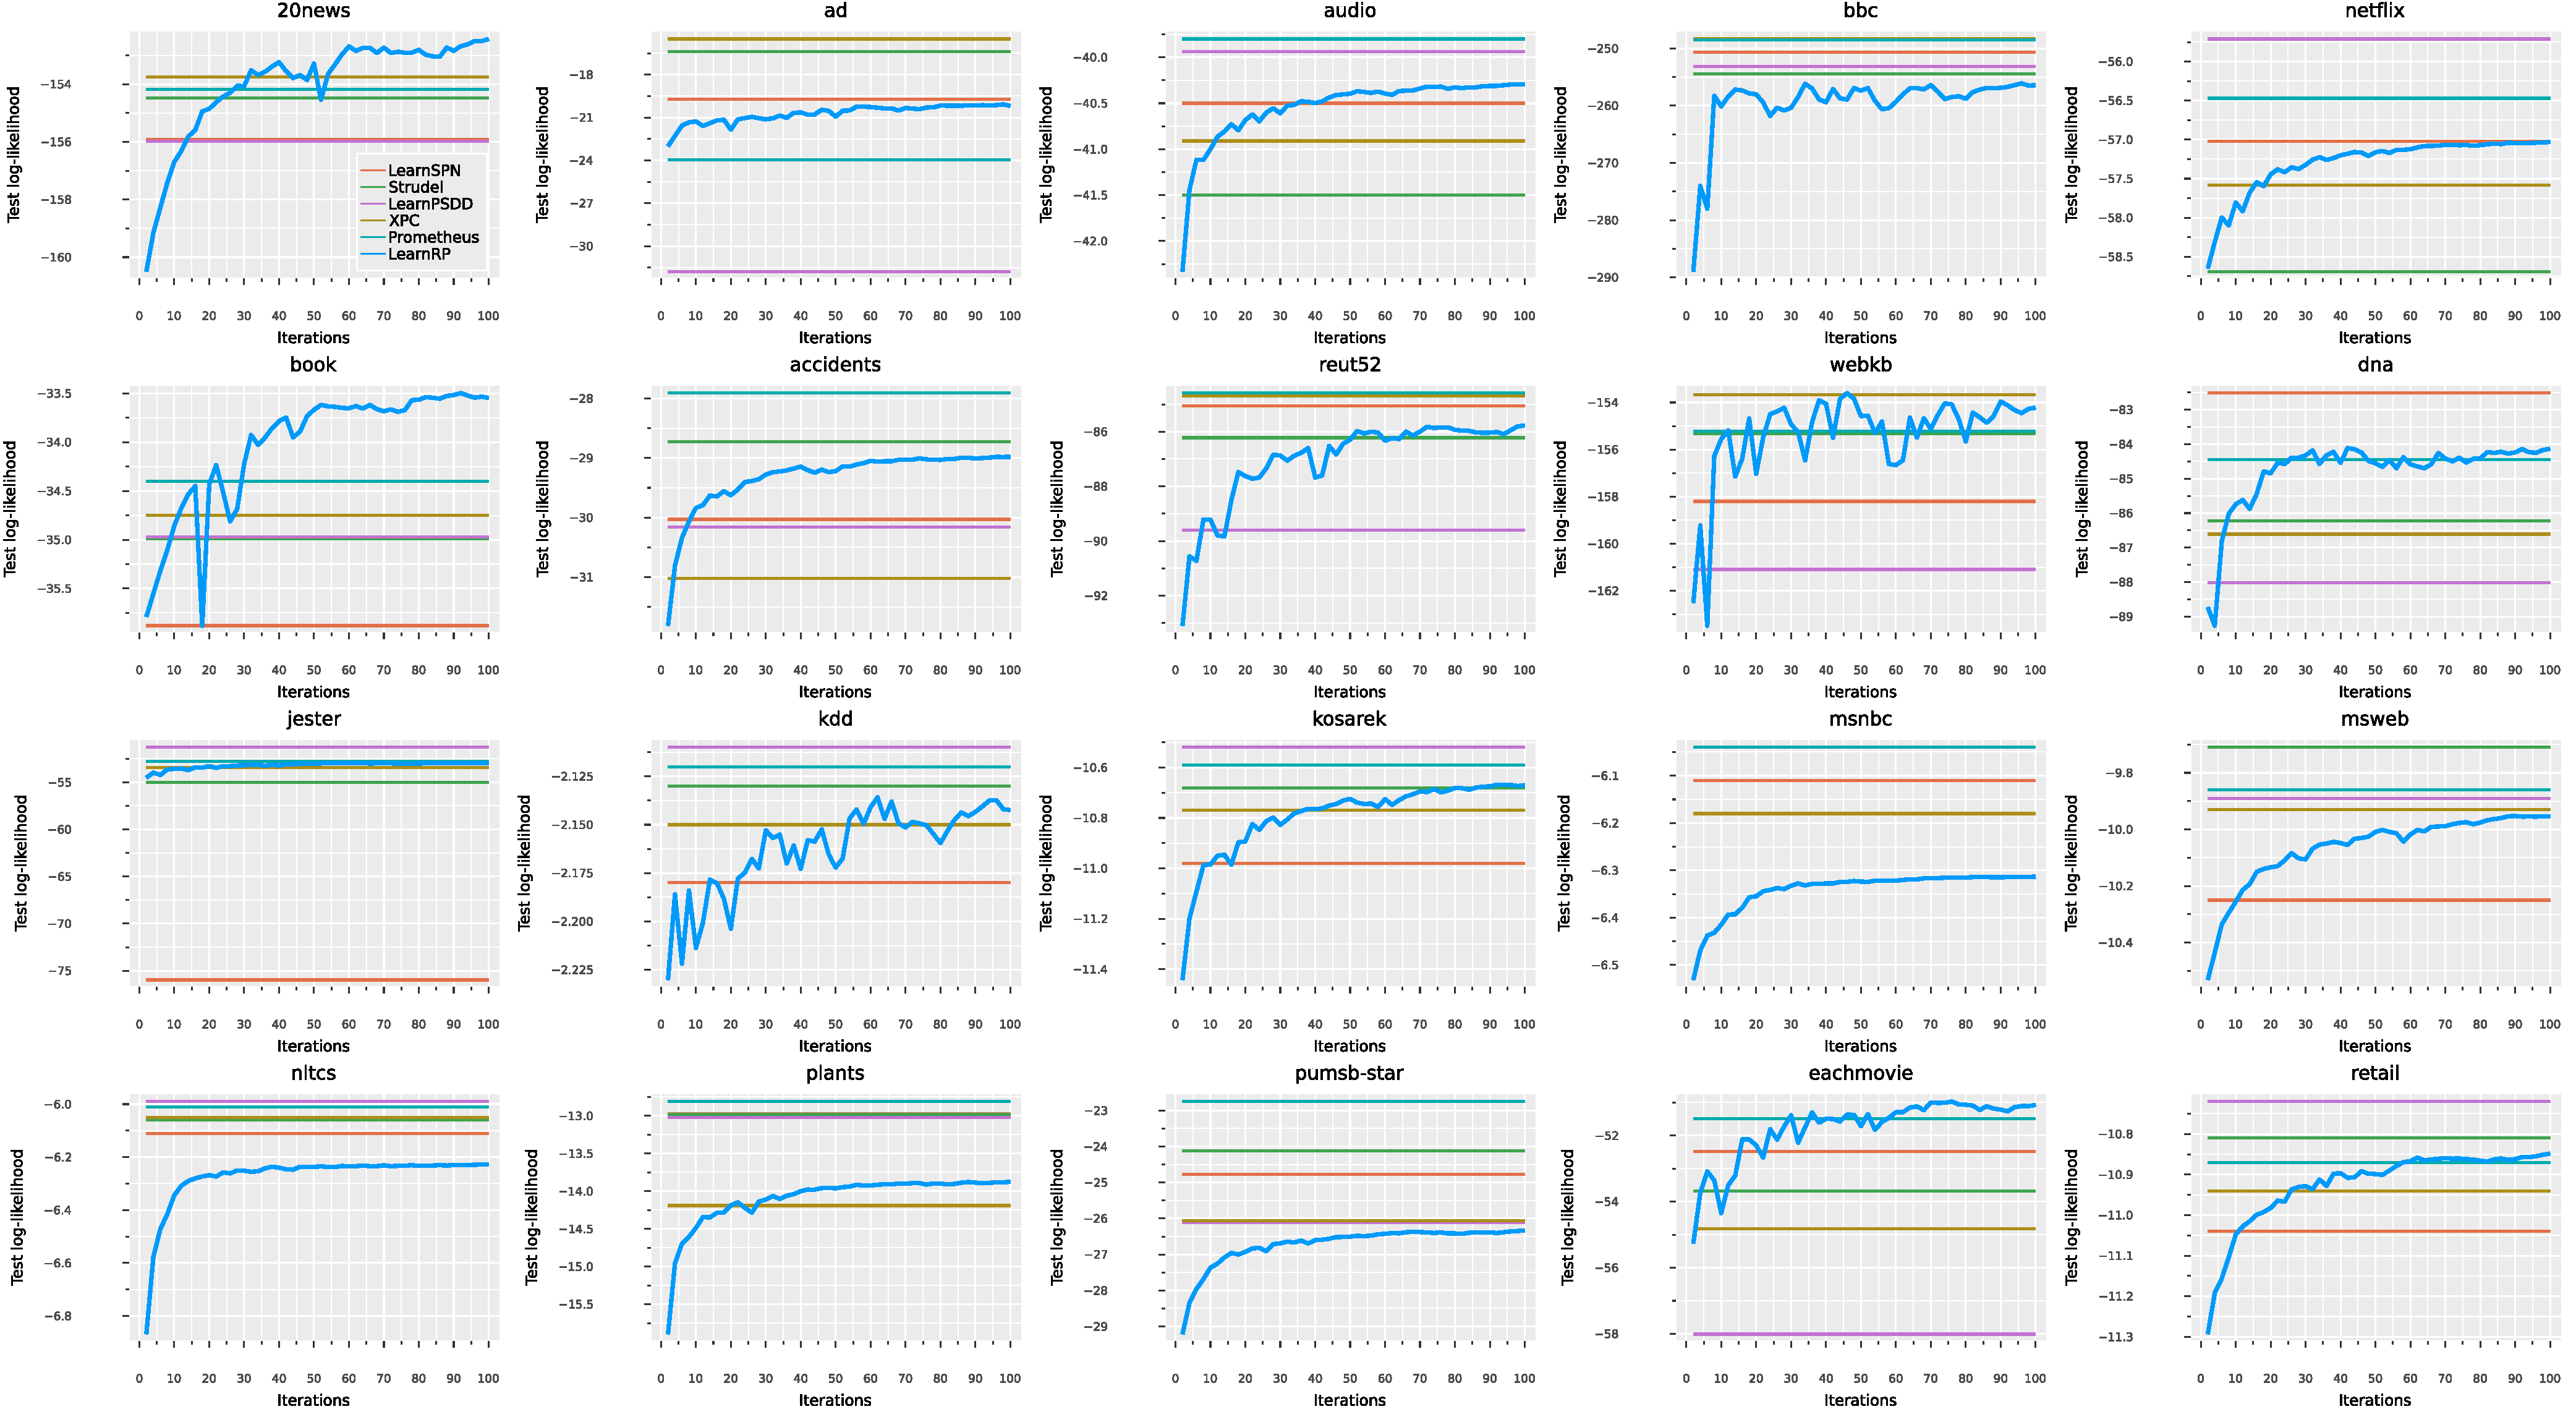
\includegraphics[height=0.9\textheight]{figures/all_slides.pdf}
\end{vhcenterb}

% Slide: Experiments 6

\newpage

\newtitle{Experiments}

\begin{vhcenterb}
  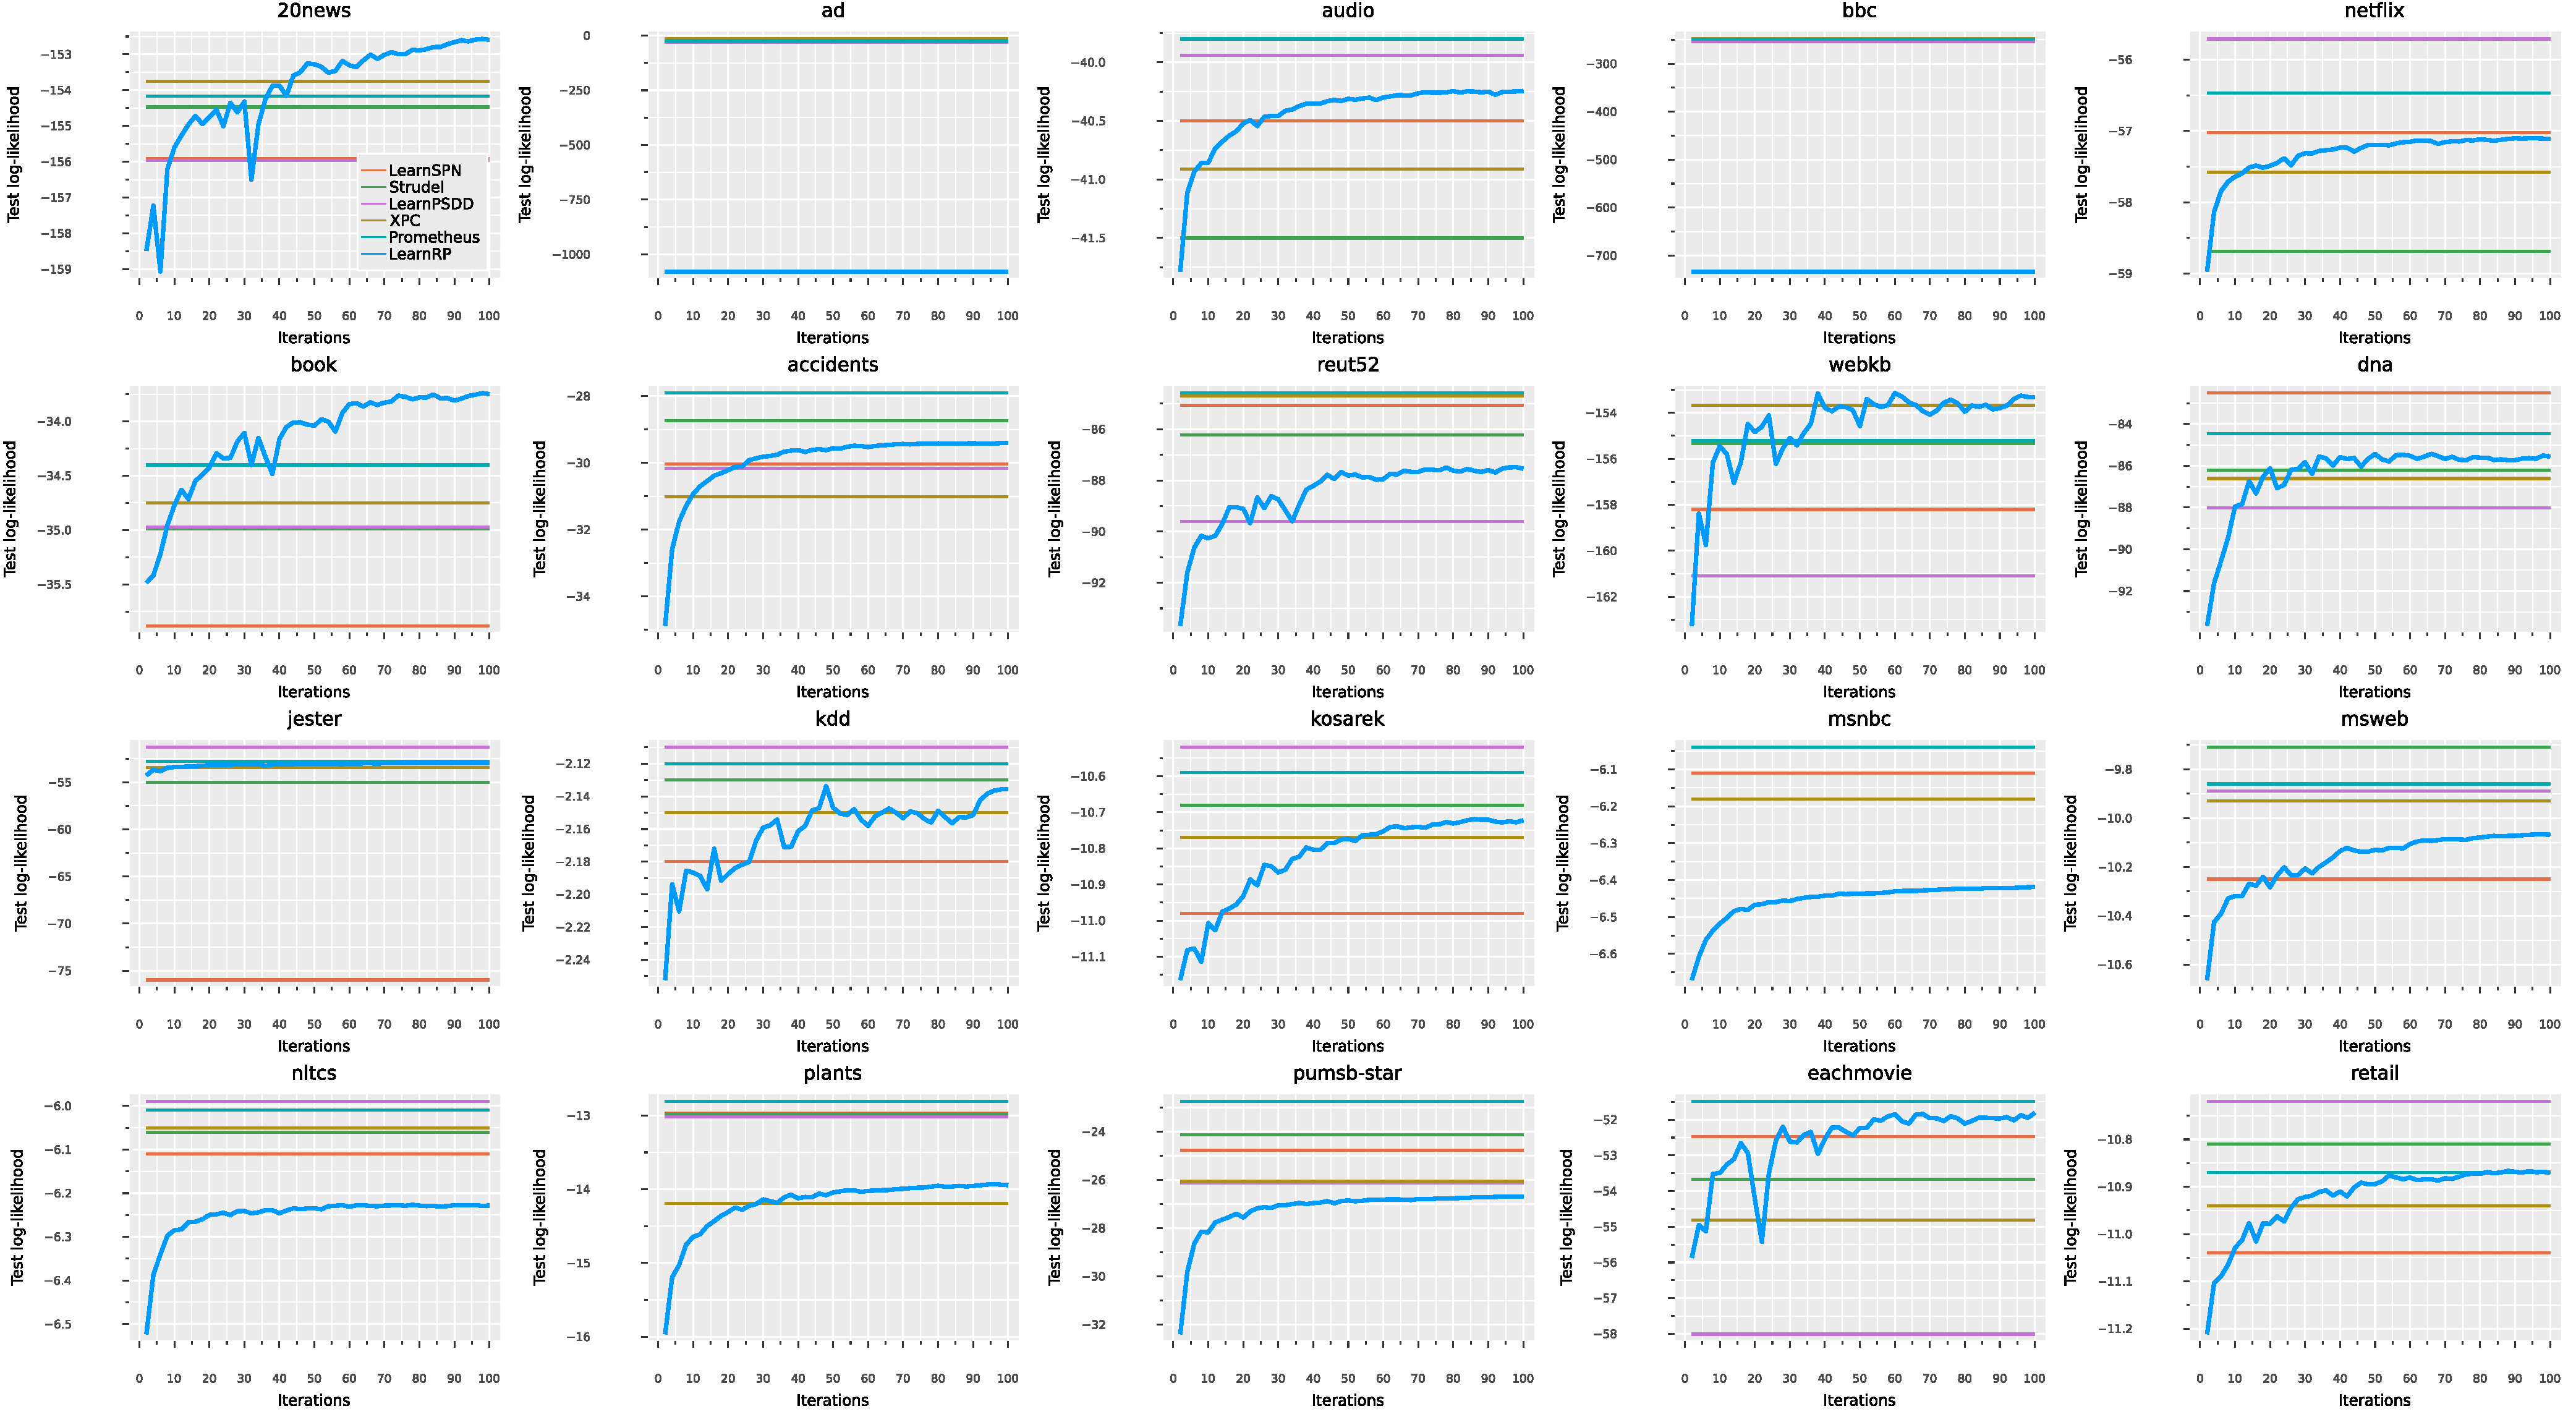
\includegraphics[height=0.9\textheight]{figures/all_rand_slides.pdf}
\end{vhcenterb}

% Slide: Experiments 7

\newpage

\newtitle{Experiments}

\begin{vhcenterb}
  \resizebox{0.9\textwidth}{!}{
    \begin{tabular}{cc|ccccccc|cc}
      \hline
      \textbf{Dataset} & \textbf{Vars} & \textbf{SRBMs} & \textbf{oSLRAU} & \textbf{GBMMs} & \textbf{iGMMs} &
      \textbf{GMMs} & \textbf{\textproc{Prometheus}} & \textbf{iSPTs} & \textbf{\textproc{LearnRP}} &
      \textbf{Size} \\
      \hline
      \textsc{abalone}    & 8  & -2.28  & $|$-0.94$|$  & -1.17  & ---   & \textbf{-0.59}   & \underline{-0.85}   & ---   & -6.13  & 317   \\
      \textsc{ca}         & 22 & -4.95  & \underline{21.19}  & $|$3.42$|$   & ---   & -1.08   & \textbf{27.82}   & ---   & -5.84  & 2765  \\
      \textsc{quake}      & 4  & -2.38  & \underline{-1.21}  & -3.76  & ---   & \textbf{-0.58}   & $|$-1.50$|$   & ---   & -3.76  & 79    \\
      \textsc{sensorless} & 48 & -26.91 & \underline{60.72}  & $|$8.56$|$   & ---   & -1.39   & \textbf{62.03}   & ---   & -38.46 & 12589 \\
      \textsc{banknote}   & 4  & -2.76  & \underline{-1.39}  & -4.64  & ---   & \textbf{-1.05}   & $|$-1.96$|$   & ---   & -6.06  & 79    \\
      \textsc{flowsize}   & 3  & -0.79  & \underline{15.32}  & $|$5.72$|$   & ---   & -36.50  & \textbf{18.03}   & ---   & 2.20   & 49    \\
      \textsc{kinematics} & 8  & \textbf{-5.55}  & -11.13 & -11.20 & ---   & \underline{-6.11}   & -11.12  & ---   & $|$-11.02$|$ & 319   \\
      \textsc{iris}       & 4  & ---    & ---    & ---    & -3.94 & \textbf{0.20}    & \underline{-1.06}   & -3.74 & $|$-3.47$|$  & 79    \\
      \textsc{oldfaith}   & 2  & ---    & ---    & ---    & $|$-1.73$|$ & -2.09   & \textbf{-1.48}   & \underline{-1.70} & -4.33  & 19    \\
      \textsc{chemdiabet} & 3  & ---    & ---    & ---    & -3.02 & \textbf{-0.58}   & \underline{-2.59}   & $|$-2.88$|$ & -18.68 & 48    \\
      \hline
    \end{tabular}
  }
\end{vhcenterb}

\nobibliography{refs.bib}

\end{document}
